\documentclass[12pt,a4paper]{article}
\usepackage{ctex}
\usepackage{amsmath,amsfonts,amssymb}
\usepackage{graphicx}
\usepackage{geometry}
\usepackage{tikz}
\usepackage{caption}
\usetikzlibrary{shapes, arrows.meta, positioning}
\usepackage{pgfplots}
\usepackage{enumerate}
\usepackage{enumitem}
\usepackage{fancyhdr}
\usepackage{hyperref}
\usepackage{tcolorbox}
\usepackage{adjustbox}
\usepackage{xcolor}
\usepackage{colortbl}
\usepackage{array}
\usepackage{multirow}
\usepackage{longtable}
\usepackage[pgf]{bodeplot}

\pgfplotsset{compat=1.18}
% allow dropping of unbounded coordinates in all plots
\pgfplotsset{unbounded coords=jump}

% 页面设置
\geometry{left=2.5cm,right=2.5cm,top=2.5cm,bottom=2.5cm,headheight=15pt}
\pagestyle{fancy}
\fancyhf{}
\rhead{\thepage}
\lhead{控制理论笔记}

% 标题设置
\title{\textbf{控制理论笔记}\\[0.5em]\large 经典控制理论与现代控制理论}
\author{学习笔记}
\date{\today}

% 定义一些常用命令
\newcommand{\laplace}{\mathcal{L}}
\newcommand{\fourier}{\mathcal{F}}
\newcommand{\jw}{\mathrm{j}\omega}

\begin{document}

\maketitle
\tableofcontents
\newpage

\part{经典控制理论}

% ==================== 基础理论 ====================
\section{自动控制系统的一般概念}

\subsection{控制系统的基本组成}
控制系统一般由以下几个基本组成部分构成:
\begin{itemize}
    \item \textbf{被控对象(控制对象)}:需要被控制的系统或装置
    \item \textbf{控制器}:对输入信号进行处理,产生控制信号
    \item \textbf{传感器}:检测被控量的实际值
    \item \textbf{执行器}:接收控制信号,对被控对象施加控制作用
\end{itemize}

\subsection{控制系统的基本要求}
\begin{enumerate}
    \item \textbf{稳定性}:系统在扰动作用下能够恢复到平衡状态
    \item \textbf{准确性}:系统的稳态误差要小
    \item \textbf{快速性}:系统的动态响应要快
\end{enumerate}


\section{自动控制系统的分类}
\label{sec:classification}

\subsection{按输入信号分类}
\begin{itemize}
    \item \textbf{恒值控制系统}:输入信号为常值
    \item \textbf{随动控制系统}:输入信号为时变信号
    \item \textbf{程序控制系统}:输入信号按预定程序变化
\end{itemize}

\subsection{按系统结构分类}
\begin{itemize}
    \item \textbf{开环控制系统}:控制装置与被控对象之间没有反馈回路
    \item \textbf{闭环控制系统}:控制装置与被控对象之间存在反馈回路
\end{itemize}

\subsection{按系统特性分类}
\begin{itemize}
    \item \textbf{线性系统与非线性系统}
    \item \textbf{定常系统与时变系统}
    \item \textbf{连续系统与离散系统}
    \item \textbf{单变量系统与多变量系统}
\end{itemize}



% ==================== 数学工具 ====================
\section{拉普拉斯变换及其性质}

\subsection{拉普拉斯变换定义}
函数 $f(t)$ 的拉普拉斯变换定义为:
\[F(s) = \laplace[f(t)] = \int_0^{\infty} f(t)e^{-st} dt\]

其中 $s = \sigma + j\omega$ 为复变量。

\subsection{基本函数的拉普拉斯变换}
\begin{align}
\laplace[\delta(t)] &= 1 \\
\laplace[1(t)] &= \frac{1}{s} \\
\laplace[t] &= \frac{1}{s^2} \\
\laplace[e^{-at}] &= \frac{1}{s+a} \\
\laplace[\sin(\omega t)] &= \frac{\omega}{s^2+\omega^2} \\
\laplace[\cos(\omega t)] &= \frac{s}{s^2+\omega^2}
\end{align}

\subsection{拉普拉斯变换的性质}
\begin{itemize}
    \item \textbf{线性性质}:$\laplace[af_1(t) + bf_2(t)] = aF_1(s) + bF_2(s)$
    \item \textbf{时移性质}:$\laplace[f(t-\tau)] = e^{-s\tau}F(s)$
    \item \textbf{频移性质}:$\laplace[e^{-at}f(t)] = F(s+a)$
    \item \textbf{微分性质}:$\laplace[f'(t)] = sF(s) - f(0^-)$
    \item \textbf{积分性质}:$\laplace[\int_0^t f(\tau)d\tau] = \frac{F(s)}{s}$
    \item \textbf{初值定理}:$f(0^+) = \lim_{s \to \infty} sF(s)$
    \item \textbf{终值定理}:$f(\infty) = \lim_{s \to 0} sF(s)$(当极限存在时)
\end{itemize}

\section{微分方程和传递函数}
\label{sec:classical-transfer-function}

\subsection{传递函数定义}
在零初始条件下,线性定常系统输出量的拉普拉斯变换与输入量的拉普拉斯变换之比称为传递函数:
\[G(s) = \frac{Y(s)}{X(s)} = \frac{b_m s^m + b_{m-1}s^{m-1} + \cdots + b_1 s + b_0}{a_n s^n + a_{n-1}s^{n-1} + \cdots + a_1 s + a_0}\]

\subsection{传递函数的性质}
\begin{itemize}
    \item 传递函数是复变量 $s$ 的有理真分式
    \item 传递函数的系数完全由系统的结构和参数决定
    \item 传递函数与输入信号无关
    \item 传递函数可以表征系统的动态特性
\end{itemize}

\section{结构图与信号流图}

\subsection{结构图的基本元件}
\begin{itemize}
    \item \textbf{方块}:表示系统或环节的传递函数
    \item \textbf{信号线}:表示信号的传输方向
    \item \textbf{相加点}:表示信号的相加或相减
    \item \textbf{分支点}:表示信号的分叉
\end{itemize}

\subsection{结构图的等效变换}
\begin{itemize}
    \item 串联:$G(s) = G_1(s)G_2(s)$
    \item 并联:$G(s) = G_1(s) + G_2(s)$
    \item 反馈:$G(s) = \frac{G_1(s)}{1 \pm G_1(s)H(s)}$
\end{itemize}

\subsection{信号流图}
信号流图是用有向线段和节点组成的图形,用来表示系统各变量之间的关系。

\section{梅森公式求传递函数}
\label{sec:mason-formula}

\subsection{梅森增益公式}
\[G(s) = \frac{1}{\Delta} \sum_{k=1}^{N} P_k \Delta_k\]

其中:
\begin{itemize}
    \item $P_k$:第 $k$ 条前向通路的增益
    \item $\Delta$:信号流图的特征式
    \item $\Delta_k$:在信号流图中划去第 $k$ 条前向通路后的特征式
\end{itemize}

\subsection{特征式的计算}
\[\Delta = 1 - \sum L_i + \sum L_i L_j - \sum L_i L_j L_k + \cdots\]

其中 $L_i$ 为各个回路的增益,相互接触的回路不能同时出现在同一项中。


% ==================== 时域分析方法 ====================
\section{时域性能指标}
\label{sec:time-domain-performance}

\subsection{典型输入信号}
\begin{itemize}
    \item \textbf{阶跃输入}:$r(t) = A \cdot 1(t)$
    \item \textbf{斜坡输入}:$r(t) = At$
    \item \textbf{抛物线输入}:$r(t) = \frac{1}{2}At^2$
    \item \textbf{脉冲输入}:$r(t) = A\delta(t)$
\end{itemize}

\subsection{时域性能指标}
对于单位阶跃响应,主要性能指标包括:
\begin{itemize}
    \item \textbf{上升时间} $t_r$:响应从终值的10%上升到90%所需的时间
    \item \textbf{峰值时间} $t_p$:响应达到第一个峰值的时间
    \item \textbf{调节时间} $t_s$:响应进入并保持在终值±2%(或±5%)范围内所需的时间
    \item \textbf{超调量} $\sigma\% = \frac{h(t_p) - h(\infty)}{h(\infty)} \times 100\%$
\end{itemize}


\section{一阶系统时域分析}
\label{sec:first-order-system}

\subsection{一阶系统的传递函数}
\[G(s) = \frac{K}{Ts + 1}\]

其中 $K$ 为增益,$T$ 为时间常数。

\subsection{一阶系统的单位阶跃响应}
\[h(t) = K(1 - e^{-t/T})\]

\subsection{一阶系统的性能指标}
\begin{itemize}
    \item 调节时间:$t_s = 3T$(2\%误差带)或 $t_s = 4T$(5\%误差带)
    \item 无超调
    \item 上升时间:$t_r = 2.2T$
\end{itemize}

\section{二阶系统时域分析}

\subsection{二阶系统的标准形式}
\[G(s) = \frac{\omega_n^2}{s^2 + 2\zeta\omega_n s + \omega_n^2}\]

其中:
\begin{itemize}
    \item $\omega_n$:无阻尼自然频率
    \item $\zeta$:阻尼比
\end{itemize}

\subsection{二阶系统的特征根}
特征方程:$s^2 + 2\zeta\omega_n s + \omega_n^2 = 0$

特征根:$s_{1,2} = -\zeta\omega_n \pm \omega_n\sqrt{\zeta^2 - 1}$

\subsection{二阶系统的分类}
\begin{itemize}
    \item $\zeta > 1$:过阻尼系统
    \item $\zeta = 1$:临界阻尼系统
    \item $0 < \zeta < 1$:欠阻尼系统
    \item $\zeta = 0$:无阻尼系统
    \item $\zeta < 0$:负阻尼系统(不稳定)
\end{itemize}

\subsection{欠阻尼二阶系统的性能指标}
\begin{align}
t_p &= \frac{\pi}{\omega_n\sqrt{1-\zeta^2}} \\
\sigma_{\%} &= e^{-\frac{\pi\zeta}{\sqrt{1-\zeta^2}}} \times 100\% \\
t_s &= \frac{3}{\zeta\omega_n} \text{(2\%误差带)}
\end{align}

\subsection{欠阻尼二阶系统的 s 平面分析}

\subsubsection{抽象参数表示}

特征根为 $s_{1,2} = -\zeta\omega_n \pm j\omega_n\sqrt{1-\zeta^2}$,在 s 平面上的几何意义如下:

\begin{tcolorbox}[colback=blue!5!white,colframe=blue!75!black,title=欠阻尼二阶系统的特征根分布,boxsep=3pt,left=3pt,right=3pt,top=3pt,bottom=3pt]

\centering
\begin{tikzpicture}
\draw[thick] (-3,0) -- (1,0) node[right] {实部 $\sigma$};
\draw[thick] (0,-3.5) -- (0,3.5) node[above] {虚部 $j\omega$};

% 绘制圆(半径为 ω_n,示例:ω_n=2)
\draw[dashed, gray, thick] (0,0) circle (2cm);

% 特征根位置(示例:ζ=0.5, ω_n=2)
\filldraw[red] (-1, 1.732) circle (3pt);
\filldraw[red] (-1, -1.732) circle (3pt);

% 从原点到特征根的连线(模为 ω_n)
\draw[black, thin, dashed] (0, 0) -- (-1, 1.732);
\draw[black, thin, dashed] (0, 0) -- (-1, -1.732);

% 从虚轴垂直线到特征根
\draw[blue, thin, line width=1.5pt] (-1, 0) -- (-1, 1.732);
\draw[blue, thin, line width=1.5pt] (-1, 0) -- (-1, -1.732);

% 虚部水平线
\draw[green!60!black, thin, line width=1.5pt] (-1, 1.732) -- (-0.5, 1.732);
\draw[green!60!black, thin, line width=1.5pt] (-1, -1.732) -- (-0.5, -1.732);

% 标注
\node[blue, font=\small, below left] at (-1, 0) {$-\zeta\omega_n$};
\node[green!60!black, font=\small, above right] at (-1, 1.732) {$j\omega_d$};
\node[green!60!black, font=\small, below right] at (-1, -1.732) {$-j\omega_d$};
\node[black, font=\small, right] at (-0.2, 0.3) {$\theta$};

% 图例
\node[font=\small] at (0.2, 2.5) {模 $|\omega_n|$};
\node[blue, font=\small] at (0.2, 2.2) {实部 $-\zeta\omega_n$};
\node[green!60!black, font=\small] at (0.2, 1.9) {虚部 $\pm\omega_d$};
\end{tikzpicture}

\textbf{参数几何意义}:\quad
{\large$\bullet$} \textbf{模} $|\omega_n|$ $\Rightarrow$ 原点到特征根距离 $\Rightarrow$ \textbf{自然频率大小}
\quad {\large$\bullet$} \textbf{实部} $-\zeta\omega_n$ $\Rightarrow$ 衰减系数 $\Rightarrow$ \textbf{衰减快慢}
\quad {\large$\bullet$} \textbf{虚部} $\pm\omega_d$ $\Rightarrow$ 震荡频率 $\Rightarrow$ \textbf{震荡速度}
\quad {\large$\bullet$} \textbf{角度} $\theta$ $\Rightarrow$ $\cos\theta = \zeta$ $\Rightarrow$ \textbf{由阻尼比确定}

\end{tcolorbox}

\subsubsection{具体示例:$G(s) = \frac{25}{s^2 + 5s + 25}$}

\begin{tcolorbox}[colback=green!5!white,colframe=green!75!black,title={具体例:欠阻尼二阶系统 $G(s) = \frac{25}{s^2+5s+25}$},boxsep=3pt,left=3pt,right=3pt,top=3pt,bottom=3pt]

\begin{minipage}[b]{0.58\textwidth}
\centering
\begin{tikzpicture}
\begin{axis}[
    width=\textwidth,
    height=6cm,
    xlabel={实部 $\sigma$ (rad/s)},
    ylabel={虚部 $j\omega$ (rad/s)},
    grid=both,
    grid style={gray!30},
    axis lines=middle,
    xmin=-6, xmax=1,
    ymin=-6, ymax=6,
    xtick={-5,-2.5,0},
    ytick={-5,-2.5,0,2.5,5},
    ticklabel style={font=\small},
    title={特征根分布},
    font=\small
]

% 圆表示 ω_n=5
\addplot[gray, dashed, thick, domain=0:360, samples=150] 
    ({5*cos(x)}, {5*sin(x)});

% 特征根
\addplot[red, mark=*, mark size=7pt, only marks] 
    coordinates {(-2.5, 4.33) (-2.5, -4.33)};

% 连线
\addplot[black, dashed, thin] coordinates {(0, 0) (-2.5, 4.33)};
\addplot[black, dashed, thin] coordinates {(0, 0) (-2.5, -4.33)};

% 实部线
\addplot[blue, thin, line width=1.5pt] coordinates {(-2.5, 0) (-2.5, 4.33)};
\addplot[blue, thin, line width=1.5pt] coordinates {(-2.5, 0) (-2.5, -4.33)};

% 虚部线
\addplot[green!60!black, thin, line width=1.5pt] coordinates {(-2.5, 4.33) (-1, 4.33)};
\addplot[green!60!black, thin, line width=1.5pt] coordinates {(-2.5, -4.33) (-1, -4.33)};

% 标注
\node[blue, font=\small, below] at (-2.5, -0.7) {$-2.5$};
\node[green!60!black, font=\small, above left] at (-2.5, 4.33) {$-2.5+j4.33$};
\node[green!60!black, font=\small, below left] at (-2.5, -4.33) {$-2.5-j4.33$};

% 角度
\addplot[orange, thick, domain=0:60, samples=40] 
    ({5*cos(x)}, {5*sin(x)});
\node[orange, font=\small] at (1.5, 1.5) {$60°$};

\end{axis}
\end{tikzpicture}
\end{minipage}\hfill
\begin{minipage}[b]{0.39\textwidth}
\small

\textbf{参数识别}:
\begin{align*}
\boldsymbol{\omega_n} &\mathbf{= 5 \text{ rad/s}} \quad (\text{自然频率}) \\
\boldsymbol{\zeta} &\mathbf{= 0.5} \quad (\text{阻尼比}) \\
\boldsymbol{\omega_d} &\mathbf{= 4.33 \text{ rad/s}} \quad (\text{震荡频率})
\end{align*}

\textbf{性能指标}:
\begin{align*}
\mathbf{t_p} &\mathbf{= 0.725 \text{ s}} \quad \text{(峰值时刻)} \\
\mathbf{\sigma_\%} &\mathbf{= 16.3\%} \quad \text{(超调量)} \\
\mathbf{t_s} &\mathbf{= 1.2 \text{ s}} \quad \text{(稳定时间)}
\end{align*}

\textbf{特征根位置}:
$$\mathbf{s_{1,2} = -2.5 \pm j4.33}$$
\vspace{0.2cm}

{\small \textit{$-2.5$:衰减速率  \quad $4.33$:震荡速度}}

\end{minipage}

\end{tcolorbox}
\section{稳定性分析及劳斯稳定判据}

\subsection{系统稳定性的定义}
线性系统稳定的充分必要条件是:系统特征方程的所有根都具有负实部,即所有特征根都位于 $s$ 平面的左半部分。

\subsection{劳斯稳定判据}
对于特征方程:
\[a_n s^n + a_{n-1}s^{n-1} + \cdots + a_1 s + a_0 = 0\]

构造劳斯表:
\begin{center}
\begin{tabular}{c|cccc}
$s^n$ & $a_n$ & $a_{n-2}$ & $a_{n-4}$ & $\cdots$ \\
$s^{n-1}$ & $a_{n-1}$ & $a_{n-3}$ & $a_{n-5}$ & $\cdots$ \\
$s^{n-2}$ & $b_1$ & $b_2$ & $b_3$ & $\cdots$ \\
$\vdots$ & $\vdots$ & $\vdots$ & $\vdots$ & $\ddots$ \\
\end{tabular}
\end{center}

其中:$b_1 = \frac{a_{n-1}a_{n-2} - a_n a_{n-3}}{a_{n-1}}$

\textbf{劳斯稳定判据}:系统稳定的充分必要条件是劳斯表第一列的元素全部为正。

\subsection{特殊情况的处理}
\begin{itemize}
    \item 第一列出现零元素:用小正数 $\varepsilon$ 代替
    \item 某一行全为零:用前一行的辅助方程的导数代替
\end{itemize}
\section{线性定常系统的稳态误差计算}
\label{sec:steady-state-error}

\subsection{误差信号和误差传递函数}
误差信号:$E(s) = R(s) - H(s)Y(s)$

误差传递函数:$\Phi_e(s) = \frac{E(s)}{R(s)} = \frac{1}{1 + G(s)H(s)}$

\subsection{系统类型}
根据开环传递函数 $G(s)H(s)$ 在原点处的极点个数确定系统类型:
\[G(s)H(s) = \frac{K \prod_{i=1}^{m}(s - z_i)}{s^\nu \prod_{j=1}^{n}(s - p_j)}\]

$\nu$ 为系统的型别。

\subsection{稳态误差系数}
\begin{itemize}
    \item \textbf{位置误差系数}:$K_p = \lim_{s \to 0} G(s)H(s)$
    \item \textbf{速度误差系数}:$K_v = \lim_{s \to 0} s \cdot G(s)H(s)$
    \item \textbf{加速度误差系数}:$K_a = \lim_{s \to 0} s^2 \cdot G(s)H(s)$
\end{itemize}

\subsection{稳态误差}
\begin{itemize}
    \item 单位阶跃输入:$e_{ss} = \frac{1}{1 + K_p}$
    \item 单位斜坡输入:$e_{ss} = \frac{1}{K_v}$
    \item 单位抛物线输入:$e_{ss} = \frac{1}{K_a}$
\end{itemize}


% ==================== 根轨迹分析方法 ====================
\section{根轨迹基本概念及其绘制(180°)}

\subsection{根轨迹的定义}
当系统中某一参数从零变化到无穷大时,闭环系统特征方程的根在 $s$ 平面上的运动轨迹称为根轨迹。

\subsection{根轨迹方程}
闭环特征方程:$1 + KG(s)H(s) = 0$

根轨迹方程的两个条件:
\begin{itemize}
    \item \textbf{幅值条件}:$|G(s)H(s)| = \frac{1}{K}$
    \item \textbf{相角条件}:$\angle G(s)H(s) = \pm 180°(2k+1)$,$k = 0, 1, 2, \cdots$
\end{itemize}

\subsection{绘制根轨迹的基本法则}
\begin{enumerate}
    \item 根轨迹的分支数等于开环极点数 $n$ 和开环零点数 $m$ 中的较大者
    \item 根轨迹起始于开环极点,终止于开环零点(有限零点或无限远零点)
    \item 根轨迹关于实轴对称
    \item 实轴上的根轨迹:实轴上某点右侧开环实零点和实极点总数为奇数
    \item 根轨迹的渐近线:
    \begin{align}
    \sigma_a &= \frac{\sum_{i=1}^n p_i - \sum_{j=1}^m z_j}{n-m} \\
    \phi_a &= \frac{(2k+1)180°}{n-m}, \quad k = 0, 1, \cdots, n-m-1
    \end{align}
    \item 分离点的计算:$\frac{d}{ds}[G(s)H(s)] = 0$
    \item 与虚轴的交点:利用劳斯判据
\end{enumerate}

\subsection{使用 pgfplots 绘制根轨迹}

使用 pgfplots 包可以方便地绘制根轨迹。以下是一个典型示例:

\subsubsection{例1:二阶系统的根轨迹}

\begin{center}
\begin{tikzpicture}
\begin{axis}[
    width=10cm, height=8cm,
    xlabel={实部 $\sigma$},
    ylabel={虚部 $j\omega$},
    grid=both,
    unit vector ratio=1 1 1,
    title={根轨迹图:$G(s)H(s) = \frac{K}{(s+1)(s+3)}$},
    xmin=-4, xmax=1,
    ymin=-3.5, ymax=3.5,
    axis lines=middle,
    legend pos=north east
]

% 开环极点
\addplot[red, mark=x, mark size=8pt, mark options={thick}, only marks] 
    coordinates {(-1,0) (-3,0)};

% 根轨迹 - 实轴上的部分($-3$ 到 $-1$)
\addplot[blue, thick, domain=-3:-1, samples=50] {0};
\addlegendentry{根轨迹}

% 根轨迹 - 复平面部分(圆形)
\addplot[blue, thick, domain=-180:180, samples=150] 
    ({-2 + cos(x)}, {sin(x)});

% 渐近线
\addplot[dashed, gray, thick] coordinates {(-2,-3.5) (-2,3.5)};
\addlegendentry{渐近线}

% 标注极点
\node[red, font=\small] at (axis cs:-1,-0.5) {$p_1=-1$};
\node[red, font=\small] at (axis cs:-3,-0.5) {$p_2=-3$};

% 标注渐近线
\node[gray, font=\small] at (axis cs:-2,3.2) {$\sigma_a=-2$};

% 标注关键点
\node[blue, font=\tiny] at (axis cs:-0.5,0.2) {$K=0$};
\node[blue, font=\tiny] at (axis cs:-2,1.2) {$K=1$};

\end{axis}
\end{tikzpicture}
\end{center}

\textbf{参数说明}:
\begin{itemize}
    \item 开环传递函数:$G(s)H(s) = \frac{K}{(s+1)(s+3)}$
    \item 极点:$p_1 = -1$,$p_2 = -3$
    \item 渐近线中心:$\sigma_a = \frac{-1+(-3)}{2} = -2$
    \item 根轨迹类型:实轴 + 圆形轨迹
\end{itemize}

\subsubsection{例2:三阶系统的根轨迹}

\begin{center}
\begin{tikzpicture}
\begin{axis}[
    width=10cm, height=8cm,
    xlabel={实部 $\sigma$},
    ylabel={虚部 $j\omega$},
    grid=both,
    unit vector ratio=1 1 1,
    title={根轨迹图:$G(s)H(s) = \frac{K}{s(s+1)(s+3)}$},
    xmin=-4, xmax=0.5,
    ymin=-4, ymax=4,
    axis lines=middle,
    legend pos=north east
]

% 开环极点
\addplot[red, mark=x, mark size=8pt, mark options={thick}, only marks] 
    coordinates {(0,0) (-1,0) (-3,0)};

% 实轴部分:(-3, -1) 和 (-∞, 0)
\addplot[blue, thick, domain=-3:-1, samples=50] {0};
\addplot[blue, thick, domain=-4:0, samples=50] {0};
\addlegendentry{根轨迹}

% 渐近线:$\sigma_a = \frac{0-1-3}{3-0} = -\frac{4}{3}$
% 角度:$\phi_a = \frac{(2k+1) \times 180°}{3}$,$k=0,1,2$
% $\phi_a = 60°, 180°, 300°$

\addplot[dashed, gray, thick, domain=-4:2, samples=50] 
    {(tan(60)) * (x + 4/3)};
\addplot[dashed, gray, thick, domain=-4:2, samples=50] 
    {-(tan(60)) * (x + 4/3)};
\addplot[dashed, gray, thick, domain=-4:1, samples=50] {0 * x};
\addlegendentry{渐近线}

% 标注极点
\node[red, font=\small] at (axis cs:0,-0.6) {$p_3=0$};
\node[red, font=\small] at (axis cs:-1,-0.6) {$p_1=-1$};
\node[red, font=\small] at (axis cs:-3,-0.6) {$p_2=-3$};

% 标注渐近线中心
\node[gray, font=\small] at (axis cs:-4/3,3.5) {$\sigma_a=-\frac{4}{3}$};

\end{axis}
\end{tikzpicture}
\end{center}

\textbf{参数说明}:
\begin{itemize}
    \item 开环传递函数:$G(s)H(s) = \frac{K}{s(s+1)(s+3)}$
    \item 极点数 $n=3$,零点数 $m=0$
    \item 渐近线中心:$\sigma_a = \frac{0-1-3}{3-0} = -\frac{4}{3}$
    \item 渐近线角度:$\phi_a = \frac{(2k+1) \times 180°}{3}$,$k=0,1,2$
    \begin{align*}
    \phi_a &= 60°, 180°, 300°
    \end{align*}
\end{itemize}

\subsection{绘制根轨迹的步骤总结}

\begin{enumerate}
    \item \textbf{确定开环极点和零点}:在复平面上标记(极点用 × 表示,零点用 ○ 表示)
    
    \item \textbf{绘制实轴部分}:满足 \texttt{相角条件} 的实轴线段
    \begin{itemize}
        \item 实轴上某点右侧的开环零点和极点总数为奇数时,该点在根轨迹上
    \end{itemize}
    
    \item \textbf{绘制渐近线}:
    \begin{align*}
    \sigma_a &= \frac{\sum p_i - \sum z_j}{n-m} \\
    \phi_a &= \frac{(2k+1) \times 180°}{n-m}, \quad k=0,1,\cdots,n-m-1
    \end{align*}
    
    \item \textbf{计算分离点和汇合点}:解方程 $\frac{d}{ds}[G(s)H(s)] = 0$
    
    \item \textbf{确定与虚轴的交点}:使用劳斯判据或代入 $s=j\omega$
    
    \item \textbf{绘制完整轨迹}:连接各部分形成光滑曲线
\end{enumerate}

\section{0°根轨迹}

\subsection{0°根轨迹的相角条件}
$\angle G(s)H(s) = \pm 360°k$,$k = 0, 1, 2, \cdots$

\subsection{0°根轨迹与180°根轨迹的区别}
\begin{itemize}
    \item 实轴上的根轨迹:实轴上某点右侧开环实零点和实极点总数为偶数
    \item 渐近线角度:$\phi_a = \frac{360°k}{n-m}$
\end{itemize}

\section{参数根轨迹}

\subsection{参数根轨迹的定义}
当系统中某一参数变化时,系统特征方程根的变化轨迹。

\subsection{参数根轨迹的绘制方法}
\begin{enumerate}
    \item 将特征方程整理成 $1 + K_h H(s) = 0$ 的形式
    \item 将参数 $K_h$ 视为可变增益
    \item 按照常规根轨迹绘制方法进行
\end{enumerate}


% ==================== 频率域分析方法 ====================
\section{频率特性基本概念}

\subsection{频率特性的定义}
对于一个稳定的线性时不变系统,当输入一个正弦信号 $r(t) = A_{\text{in}}\sin(\omega t)$ 时,其稳态输出 $y_{\text{ss}}(t)$ 必然是同频率的正弦信号,形式为:
\[y_{\text{ss}}(t) = A_{\text{out}}\sin(\omega t + \phi)\]

线性定常系统的频率特性是指系统稳态输出与输入的复数比:
\[G(\jw) = G(s)|_{s=\jw} = |G(\jw)|e^{j\phi(\omega)}\]

其中:
\begin{itemize}
    \item \textbf{幅频特性 $A(\omega)$}:输出响应的稳态分量幅值与输入信号幅值之比。
    \[A(\omega) = \frac{A_{\text{out}}}{A_{\text{in}}} = |G(\jw)|\]
    \item \textbf{相频特性 $\phi(\omega)$}:输出响应的稳态分量与输入信号的相位之差。
    \[\phi(\omega) = \angle G(\jw)\]
\end{itemize}

幅频特性 $A(\omega)$ 和相频特性 $\phi(\omega)$ 统称为\textbf{频率特性}。

\subsection{频率特性的物理意义}
\begin{itemize}
    \item 幅频特性表示不同频率正弦输入信号通过系统后幅值的变化
    \item 相频特性表示不同频率正弦输入信号通过系统后相位的变化
\end{itemize}

\subsection{频率特性的计算}

\subsubsection{计算步骤}
\begin{enumerate}
    \item 将传递函数 $G(s)$ 中的 $s$ 替换为 $j\omega$,得到 $G(j\omega)$
    \item 计算幅频特性:$A(\omega) = |G(j\omega)|$
    \item 计算相频特性:$\phi(\omega) = \angle G(j\omega)$
\end{enumerate}

\subsubsection{例题}

\textbf{例1:已知传递函数为 $G(s)=\frac{4(s+1)}{s(s+2)}$,写出该传递函数的频率特性。}

\textit{解:}
\begin{enumerate}
    \item 将 $s$ 替换为 $j\omega$:
    \[G(j\omega)=\frac{4(j\omega+1)}{j\omega(j\omega+2)}\]
    
    \item 计算幅频特性 $A(\omega)$:
    \[A(\omega) = |G(j\omega)| = \frac{|4(1+j\omega)|}{|j\omega||2+j\omega|} = \frac{4\sqrt{1^2+\omega^2}}{\omega\sqrt{2^2+\omega^2}} = \frac{4\sqrt{1+\omega^2}}{\omega\sqrt{4+\omega^2}}\]
    
    \item 计算相频特性 $\phi(\omega)$:
    \begin{align*}
    \phi(\omega) &= \angle G(j\omega) = \angle 4 + \angle(1+j\omega) - \angle(j\omega) - \angle(2+j\omega) \\
    &= 0° + \arctan(\omega) - 90° - \arctan(\frac{\omega}{2}) \\
    &= \arctan(\omega) - \arctan(\frac{\omega}{2}) - 90°
    \end{align*}
\end{enumerate}

\textbf{例2:某单位负反馈的开环传递函数为 $G(s)=\frac{4}{s(s+2)}$。若输入信号 $r(t)=2\sin(2t)$,试求系统的稳态输出。}

\textit{解:}
\begin{enumerate}
    \item 求闭环传递函数 $\Phi(s)$:
    \[\Phi(s) = \frac{G(s)}{1+G(s)} = \frac{\frac{4}{s(s+2)}}{1+\frac{4}{s(s+2)}} = \frac{4}{s^2+2s+4}\]
    
    \item 分析输入信号:幅值 $A=2$,角频率 $\omega=2$ rad/s
    
    \item 计算闭环系统在 $\omega=2$ 处的频率响应 $\Phi(j2)$:
    \[\Phi(j2) = \frac{4}{(j2)^2+2(j2)+4} = \frac{4}{-4+j4+4} = \frac{4}{j4} = -j\]
    
    \item 计算幅值和相角:
    \begin{align*}
    |\Phi(j2)| &= |-j| = 1 \\
    \angle\Phi(j2) &= \angle(-j) = -90°
    \end{align*}
    
    \item 写出稳态输出 $c_{\text{ss}}(t)$:
    \begin{align*}
    c_{\text{ss}}(t) &= A \cdot |\Phi(j2)| \cdot \sin(\omega t + \angle\Phi(j2)) \\
    &= 2 \cdot 1 \cdot \sin(2t - 90°) \\
    &= 2\sin(2t-90°) = -2\cos(2t)
    \end{align*}
\end{enumerate}

\section{奈奎斯特图绘制}

\subsection{奈奎斯特图的定义}
奈奎斯特图是以 $G(\jw)$ 的实部为横坐标,虚部为纵坐标,$\omega$ 从 $-\infty$ 到 $+\infty$ 变化时 $G(\jw)$ 在复平面上的轨迹。

\subsection{典型环节的奈奎斯特图}
\begin{itemize}
    \item \textbf{比例环节}: $G(\jw) = K$。奈奎斯特图是实轴上的一个点 $(K, 0)$。
    \item \textbf{二阶振荡环节}: 曲线形状取决于阻尼比 $\zeta$。
\end{itemize}

\subsubsection{积分环节}
积分环节的传递函数为 $G(s) = \frac{1}{s}$,其频率特性为 $G(\jw) = \frac{1}{\jw} = -\frac{j}{\omega}$。
当 $\omega$ 从 $0^+$ 变化到 $+\infty$ 时,奈奎斯特图是沿着负虚轴从 $-\infty$ 到原点的一条直线。

\begin{center}
\begin{tikzpicture}
\begin{axis}[
    width=8cm, height=8cm,
    xlabel={实部 Re},
    ylabel={虚部 Im},
    grid=both,
    unit vector ratio=1 1 1,
    title={积分环节奈奎斯特图},
    xmin=-1.5, xmax=1.5,
    ymin=-2, ymax=1,
    axis lines=middle,
    xtick={-1,0,1},
    ytick={-2,-1,0,1},
]
% Nyquist plot for 1/s
\addplot[blue, thick, ->] coordinates {(0, -0.1) (0, -2)};
\node at (axis cs:0.5, -1) {$\omega: 0^+ \to +\infty$};
\end{axis}
\end{tikzpicture}
\end{center}

\subsubsection{惯性环节}
惯性环节的传递函数为 $G(s) = \frac{1}{Ts+1}$,其频率特性为 $G(\jw) = \frac{1}{1+j\omega T}$。
奈奎斯特图是一个起点为 $(1,0)$ ($\omega=0$),终点为原点 ($\omega=\infty$) 的半圆。

\begin{center}
\begin{tikzpicture}
\begin{axis}[
    width=8cm, height=6cm,
    xlabel={实部 Re},
    ylabel={虚部 Im},
    grid=both,
    unit vector ratio=1 1 1,
    title={惯性环节奈奎斯特图},
    xmin=-0.2, xmax=1.2,
    ymin=-0.7, ymax=0.7,
    axis lines=middle,
]
% Nyquist plot for 1/(Ts+1)
\addplot[blue, thick, domain=0:10, samples=100, ->] 
    ({1/(1+x^2)}, {-x/(1+x^2)});
\node at (axis cs:0.5, -0.4) {$\omega: 0 \to \infty$};
\node at (axis cs:1, 0.1) {$\omega=0$};
\node at (axis cs:0, 0.1) {$\omega=\infty$};
\end{axis}
\end{tikzpicture}
\end{center}

\subsubsection{微分环节}
微分环节的传递函数为 $G(s) = s$,其频率特性为 $G(\jw) = j\omega$。
奈奎斯特图是沿着正虚轴从原点到 $+\infty$ 的一条直线。

\begin{center}
\begin{tikzpicture}
\begin{axis}[
    width=8cm, height=8cm,
    xlabel={实部 Re},
    ylabel={虚部 Im},
    grid=both,
    unit vector ratio=1 1 1,
    title={微分环节奈奎斯特图},
    xmin=-1.5, xmax=1.5,
    ymin=-1, ymax=2,
    axis lines=middle,
]
% Nyquist plot for s
\addplot[blue, thick, ->] coordinates {(0, 0) (0, 2)};
\node at (axis cs:0.5, 1) {$\omega: 0 \to +\infty$};
\end{axis}
\end{tikzpicture}
\end{center}

\section{伯德图绘制}

\subsection{伯德图的定义}
伯德图由两个图组成:
\begin{itemize}
    \item 幅频特性图:$L(\omega) = 20\lg|G(\jw)|$ dB vs $\lg\omega$
    \item 相频特性图:$\phi(\omega)$ vs $\lg\omega$
\end{itemize}

\subsection{典型环节的伯德图}
\begin{enumerate}
    \item \textbf{比例环节} $K$:
    \begin{itemize}
        \item $L(\omega) = 20\lg K$ dB(水平线)
        \item $\phi(\omega) = 0°$
    \end{itemize}
    
    \item \textbf{积分环节} $\frac{1}{s}$:
    \begin{itemize}
        \item $L(\omega) = -20\lg\omega$ dB(斜率-20dB/十倍频)
        \item $\phi(\omega) = -90°$
    \end{itemize}
    
    \item \textbf{一阶惯性环节} $\frac{1}{1+Ts}$:
    \begin{itemize}
        \item 转折频率:$\omega_c = \frac{1}{T}$
        \item $\omega < \omega_c$:$L(\omega) \approx 0$ dB
        \item $\omega > \omega_c$:$L(\omega) \approx -20\lg(\omega T)$ dB
        \item $\phi(\omega_c) = -45°$
    \end{itemize}
\end{enumerate}

\subsection{使用 LaTeX 绘制伯德图}
使用 \texttt{bodeplot} 包可以方便地绘制伯德图:

\subsubsection{通过零极点增益形式绘制}
\begin{center}
\begin{tikzpicture}
% 示例:G(s) = 10/((s+1)(s+10))
\begin{semilogxaxis}[
    width=10cm,height=6cm,
    xlabel={频率 $\omega$ (rad/s)},
    ylabel={幅度 (dB)},
    grid=both,
    title={幅频特性曲线}
]
\addplot+[blue,thick] coordinates {
    (1e-2, 40)
    (1e-1, 20)
    (1, 0)
    (10, -20)
    (1e2, -40)
};
\end{semilogxaxis}
\end{tikzpicture}
\end{center}

\subsubsection{相频特性绘制}
\begin{center}
\begin{tikzpicture}
\begin{semilogxaxis}[
    width=10cm,height=5cm,
    xlabel={频率 $\omega$ (rad/s)},
    ylabel={相位 (度)},
    grid=both,
    title={相频特性曲线}
]
\addplot+[red,thick] coordinates {
    (1e-2, 0)
    (1e-1, -45)
    (1, -90)
    (10, -135)
    (1e2, -180)
};
\end{semilogxaxis}
\end{tikzpicture}
\end{center}


\part{现代控制理论}

% ==================== 状态空间理论 ====================
\part{现代控制理论}

\section{状态空间表达式及其建立}

\subsection{状态空间的基本概念}
\begin{itemize}
    \item \textbf{状态}:系统在某一时刻的状态是指确定系统该时刻以后行为所必需的最少信息
    \item \textbf{状态变量}:描述系统状态的一组变量
    \item \textbf{状态向量}:由状态变量组成的向量
    \item \textbf{状态空间}:以状态变量为坐标的n维空间
\end{itemize}

\subsection{状态空间表达式}
线性定常系统的状态空间表达式:
\begin{align}
\dot{x}(t) &= Ax(t) + Bu(t) \\
\dot{y}(t) &= Cx(t) + Du(t)
\end{align}

其中:
\begin{itemize}
    \item $x(t) \in \mathbb{R}^n$:状态向量
    \item $u(t) \in \mathbb{R}^p$:输入向量
    \item $y(t) \in \mathbb{R}^q$:输出向量
    \item $A \in \mathbb{R}^{n \times n}$:系统矩阵
    \item $B \in \mathbb{R}^{n \times p}$:输入矩阵
    \item $C \in \mathbb{R}^{q \times n}$:输出矩阵
    \item $D \in \mathbb{R}^{q \times p}$:前馈矩阵
\end{itemize}

\subsection{状态空间表达式的建立方法}
\begin{enumerate}
    \item 根据物理规律建立微分方程组
    \item 选择状态变量(通常选择能量存储元件的变量)
    \item 将高阶微分方程化为一阶微分方程组
    \item 写出输出方程
\end{enumerate}

\section{状态空间表达式求传递函数}
\label{sec:transfer-function}

\subsection*{引言:搭建经典与现代的桥梁}

你已经掌握了两种系统描述方法:
\begin{itemize}
    \item \textbf{经典方法}:传递函数 $G(s)$(输入输出关系,代数)
    \item \textbf{现代方法}:状态空间 $(A, B, C, D)$(内部状态演化,微分方程组)
\end{itemize}

\textbf{现实问题:}
\begin{itemize}
    \item 已有大量基于传递函数的经典设计工具(根轨迹、频域分析)
    \item 用状态空间建模后,如何利用这些工具?
    \item 两种描述能否互相转换?
\end{itemize}

\textbf{本章核心:}从状态空间 $(A, B, C, D)$ 推导传递函数 $G(s)$。

\textbf{为什么重要?}
\begin{enumerate}
    \item \textbf{工具互通}:用状态空间建模,用传递函数分析
    \item \textbf{验证模型}:两种方法得到的极点、零点应一致
    \item \textbf{降维理解}:状态空间是 $n$ 维内部结构,传递函数是外部输入输出特性
\end{enumerate}

\textbf{本章路线:}
\begin{itemize}
    \item 单输入单输出(SISO)系统的转换公式
    \item 多输入多输出(MIMO)系统的传递函数矩阵
    \item 计算方法与实例
    \item MATLAB实现
\end{itemize}

\subsection{从状态空间到传递函数}

\subsubsection{基本推导}

考虑线性时不变系统:
\begin{align*}
\dot{x} &= Ax + Bu \\
y &= Cx + Du
\end{align*}

\textbf{目标:}求 $G(s) = \frac{Y(s)}{U(s)}$(零初始条件)

\textbf{推导步骤:}

对状态方程取拉普拉斯变换($x(0) = 0$):
\[sX(s) = AX(s) + BU(s)\]

解出 $X(s)$:
\begin{align*}
(sI - A)X(s) &= BU(s) \\
X(s) &= (sI - A)^{-1}BU(s)
\end{align*}

代入输出方程:
\begin{align*}
Y(s) &= CX(s) + DU(s) \\
&= C(sI - A)^{-1}BU(s) + DU(s) \\
&= [C(sI - A)^{-1}B + D]U(s)
\end{align*}

\textbf{传递函数公式:}
\[\boxed{G(s) = C(sI - A)^{-1}B + D}\]

\subsubsection{公式解读}

\begin{itemize}
    \item $(sI - A)^{-1}$:称为\textbf{解析矩阵}或\textbf{状态转移矩阵}(频域)
    \item $C(sI - A)^{-1}B$:状态空间部分的贡献
    \item $D$:直接传输项(输入到输出的直接通路)
    \item 通常 $D = 0$(物理系统很少有瞬时响应)
\end{itemize}

\subsubsection{计算方法}

\textbf{关键步骤:}计算 $(sI - A)^{-1}$

利用矩阵求逆公式:
\[(sI - A)^{-1} = \frac{\text{adj}(sI - A)}{\det(sI - A)}\]

其中:
\begin{itemize}
    \item $\det(sI - A)$:系统的\textbf{特征多项式}(传递函数的分母)
    \item $\text{adj}(sI - A)$:$(sI - A)$ 的伴随矩阵
\end{itemize}

\subsection{单输入单输出(SISO)系统}

\subsubsection{标准形式}

对于 SISO 系统($u, y$ 均为标量):
\[G(s) = C(sI - A)^{-1}B + D = \frac{b_m s^m + \cdots + b_1 s + b_0}{s^n + a_{n-1}s^{n-1} + \cdots + a_1 s + a_0}\]

\textbf{关键性质:}
\begin{itemize}
    \item \textbf{分母}:$\det(sI - A)$,由 $A$ 矩阵决定(系统极点)
    \item \textbf{分子}:$C \cdot \text{adj}(sI - A) \cdot B$,由 $A, B, C$ 共同决定(系统零点)
    \item \textbf{阶数}:分母阶数 = 状态维数 $n$;分子阶数 $\leq n-1$(真分式)
\end{itemize}

\subsubsection{范例1:二阶系统}

\textbf{题目:}求传递函数

给定系统:
\begin{align*}
\dot{x} &= \begin{bmatrix} 0 & 1 \\ -2 & -3 \end{bmatrix} x + \begin{bmatrix} 0 \\ 1 \end{bmatrix} u \\
y &= \begin{bmatrix} 1 & 0 \end{bmatrix} x
\end{align*}

\textbf{解答:}

\textbf{步骤1:}构造 $sI - A$
\[sI - A = \begin{bmatrix} s & -1 \\ 2 & s+3 \end{bmatrix}\]

\textbf{步骤2:}计算 $\det(sI - A)$
\[\det(sI - A) = s(s+3) - (-1)(2) = s^2 + 3s + 2\]

\textbf{步骤3:}计算 $(sI - A)^{-1}$
\[(sI - A)^{-1} = \frac{1}{s^2+3s+2}\begin{bmatrix} s+3 & 1 \\ -2 & s \end{bmatrix}\]

\textbf{步骤4:}计算 $G(s)$
\begin{align*}
G(s) &= C(sI - A)^{-1}B \\
&= \begin{bmatrix} 1 & 0 \end{bmatrix} \cdot \frac{1}{s^2+3s+2}\begin{bmatrix} s+3 & 1 \\ -2 & s \end{bmatrix} \cdot \begin{bmatrix} 0 \\ 1 \end{bmatrix} \\
&= \frac{1}{s^2+3s+2}\begin{bmatrix} 1 & 0 \end{bmatrix}\begin{bmatrix} 1 \\ s \end{bmatrix} \\
&= \boxed{\frac{1}{s^2+3s+2}}
\end{align*}

\textbf{验证:}极点为 $s = -1, -2$(特征值),无零点。

\subsection{多输入多输出(MIMO)系统}

\subsubsection{传递函数矩阵}

对于 $p$ 输出、$m$ 输入系统:
\[G(s) = C(sI - A)^{-1}B + D \in \mathbb{R}^{p \times m}(s)\]

\textbf{矩阵元素:}
\[G_{ij}(s) = \frac{Y_i(s)}{U_j(s)}\Big|_{\text{其他输入为0}}\]

表示第 $j$ 个输入到第 $i$ 个输出的传递函数。

\subsubsection{范例2:MIMO系统}

\textbf{题目:}双输入双输出系统

\begin{align*}
A = \begin{bmatrix} -1 & 0 \\ 0 & -2 \end{bmatrix}, \quad
B = \begin{bmatrix} 1 & 0 \\ 0 & 1 \end{bmatrix}, \quad
C = \begin{bmatrix} 1 & 1 \\ 0 & 1 \end{bmatrix}, \quad
D = 0
\end{align*}

\textbf{解答:}

\textbf{步骤1:}$(sI - A)^{-1}$ 对角矩阵
\[(sI - A)^{-1} = \begin{bmatrix} \frac{1}{s+1} & 0 \\ 0 & \frac{1}{s+2} \end{bmatrix}\]

\textbf{步骤2:}计算 $G(s)$
\begin{align*}
G(s) &= C(sI - A)^{-1}B \\
&= \begin{bmatrix} 1 & 1 \\ 0 & 1 \end{bmatrix} \begin{bmatrix} \frac{1}{s+1} & 0 \\ 0 & \frac{1}{s+2} \end{bmatrix} \begin{bmatrix} 1 & 0 \\ 0 & 1 \end{bmatrix} \\
&= \boxed{\begin{bmatrix} \frac{1}{s+1} & \frac{1}{s+2} \\ 0 & \frac{1}{s+2} \end{bmatrix}}
\end{align*}

\textbf{解释:}
\begin{itemize}
    \item $G_{11}(s) = \frac{1}{s+1}$:输入1 → 输出1
    \item $G_{12}(s) = \frac{1}{s+2}$:输入2 → 输出1
    \item $G_{21}(s) = 0$:输入1对输出2无影响
    \item $G_{22}(s) = \frac{1}{s+2}$:输入2 → 输出2
\end{itemize}

\subsection{MATLAB实现}

\textbf{方法1:直接使用 \texttt{ss2tf}}

\begin{lstlisting}[style=Matlab-editor]
% 定义状态空间模型
A = [0 1; -2 -3];
B = [0; 1];
C = [1 0];
D = 0;

% 转换为传递函数
[num, den] = ss2tf(A, B, C, D);

% 显示结果
G = tf(num, den)
\end{lstlisting}

\textbf{方法2:使用系统对象}

\begin{lstlisting}[style=Matlab-editor]
% 创建状态空间对象
sys_ss = ss(A, B, C, D);

% 转换为传递函数对象
sys_tf = tf(sys_ss);

% 查看传递函数
zpk(sys_tf)  % 零极点增益形式
\end{lstlisting}

\textbf{方法3:MIMO系统}

\begin{lstlisting}[style=Matlab-editor]
% MIMO系统
A = [-1 0; 0 -2];
B = [1 0; 0 1];
C = [1 1; 0 1];
D = zeros(2,2);

sys_ss = ss(A, B, C, D);
sys_tf = tf(sys_ss);

% 查看传递函数矩阵
sys_tf
\end{lstlisting}

\subsection*{本章小结}

\subsubsection*{核心公式}

\begin{tcolorbox}[colback=blue!5!white,colframe=blue!75!black,title=状态空间到传递函数]
\[\boxed{G(s) = C(sI - A)^{-1}B + D}\]

\textbf{关键步骤:}
\begin{enumerate}
    \item 构造 $sI - A$
    \item 计算 $\det(sI - A)$(特征多项式)
    \item 求 $(sI - A)^{-1}$(伴随矩阵法或直接求逆)
    \item 矩阵相乘 $C \cdot (sI-A)^{-1} \cdot B + D$
\end{enumerate}
\end{tcolorbox}

\subsubsection*{两种描述对比}

\begin{center}
\renewcommand{\arraystretch}{1.6}
\begin{tabular}{|l|p{5cm}|p{5cm}|}
\hline
\rowcolor[gray]{0.9}
\textbf{特性} & \textbf{状态空间} & \textbf{传递函数} \\
\hline
描述对象 & 内部状态演化 & 输入输出关系 \\
\hline
维度 & $n$ 维向量微分方程 & 标量代数方程 \\
\hline
适用性 & MIMO、时变、非线性 & SISO、线性时不变 \\
\hline
信息量 & 完整(状态+输入输出) & 部分(仅输入输出) \\
\hline
设计方法 & 极点配置、观测器 & 根轨迹、频域 \\
\hline
\end{tabular}
\end{center}

\subsubsection*{实际应用}

\textbf{何时需要转换?}
\begin{itemize}
    \item 用状态空间建模后,想用根轨迹/伯德图分析
    \item 验证模型:两种方法的极点应一致
    \item 简化理解:传递函数更直观显示输入输出关系
\end{itemize}

\textbf{注意事项:}
\begin{itemize}
    \item 状态空间非唯一,但传递函数唯一
    \item 不可控/不可观部分的极点会被约掉(极零对消)
    \item MIMO系统:传递函数矩阵有 $p \times m$ 个元素
\end{itemize}

\subsubsection*{与后续章节的联系}

\begin{itemize}
    \item \textbf{第\ref{sec:linear-transformation}章}:线性变换改变状态空间表示,但传递函数不变(不变性)
    \item \textbf{第\ref{sec:controllability-observability}章}:能控能观性与传递函数的极零点关系
    \item \textbf{反向转换}:传递函数 → 状态空间(能控/能观标准型)将在第\ref{sec:standard-forms}章讨论
\end{itemize}

\textbf{关键启示:}传递函数是状态空间的\textbf{外部视图},丢失了内部结构信息,但更简洁便于分析。两种描述相辅相成,需要灵活运用。

\section{线性变换}
\label{sec:linear-transformation}

\subsection*{引言:为什么需要更换 \textquotedblleft 坐标系  \textquotedblright ?}

想象你站在一个房间里观察一个旋转的陀螺。如果你从正面看,陀螺的运动可能非常复杂;但如果你沿着陀螺的旋转轴观察,运动就变得简单——只是一个圆周运动。\textbf{这就是线性变换的核心思想:通过选择合适的\textquotedblleft 观察角度 \textquotedblright(坐标系),让复杂的系统变得简单。}

\subsubsection*{为什么状态不唯一?}

在\ref{sec:state-space}节中,我们知道状态空间表达式的形式为 $\dot{x} = Ax + Bu$。但问题是:\textbf{状态变量的选择不是唯一的!}

\begin{itemize}[leftmargin=2em]
    \item \textbf{物理角度}:描述同一个系统,可以选择不同的物理量作为状态(例如位置-速度 vs 动量-能量)
    \item \textbf{数学角度}:即使选择相同的物理量,也可以用不同的坐标系表示(直角坐标 vs 极坐标)
    \item \textbf{工程角度}:某些坐标系下,系统矩阵 $A$ 的结构更简单,便于分析和设计
\end{itemize}

\subsubsection*{线性变换的作用}

线性变换(也称\textbf{坐标变换}或\textbf{相似变换})允许我们在不改变系统本质特性的前提下,\textbf{切换到更方便的坐标系}。关键性质:

\begin{tcolorbox}[colback=blue!5!white, colframe=blue!75!black, title=线性变换的不变量]
无论如何变换坐标系,以下系统特性保持不变:
\begin{itemize}
    \item \textbf{特征值}(系统的固有频率和稳定性)
    \item \textbf{传递函数}(输入输出关系)
    \item \textbf{能控性和能观性}(系统的结构性质)
\end{itemize}
\end{tcolorbox}

\subsubsection*{本章路线图}

\begin{enumerate}
    \item \textbf{数学框架}:线性变换的定义和推导
    \item \textbf{相似变换性质}:哪些量变、哪些量不变
    \item \textbf{实用例题}:如何选择变换矩阵 $P$
    \item \textbf{几何直观}:坐标变换的可视化理解
    \item \textbf{通向标准型}:为\ref{sec:standard-forms}节的标准型做准备
\end{enumerate}

\subsection{线性变换的定义}

设 $x \in \mathbb{R}^n$ 和 $z \in \mathbb{R}^n$ 是描述同一系统的两组状态变量。如果存在\textbf{非奇异矩阵} $P \in \mathbb{R}^{n \times n}$(即 $\det(P) \neq 0$,$P$ 可逆),使得:
\begin{empheq}[box=\fbox]{equation}
x = Pz
\end{empheq}

则称此变换为\textbf{线性变换}(Linear Transformation)或\textbf{坐标变换}(Coordinate Transformation)。

\subsubsection*{关键理解}

\begin{itemize}
    \item $P$ 称为\textbf{变换矩阵},它的列向量构成新坐标系的基
    \item $x$ 是原坐标系下的状态,$z$ 是新坐标系下的状态
    \item 非奇异条件 $\det(P) \neq 0$ 保证变换可逆:$z = P^{-1}x$
    \item 同一个物理系统,不同坐标下的\textquotedblleft 坐标值 \textquotedblright 不同,但描述的是同一个 \textquotedblleft 点 \textquotedblright
\end{itemize}

\subsection{变换后的状态方程}

原系统的状态空间表达式为:
\begin{align}
\dot{x} &= Ax + Bu \label{eq:original-system} \\
y &= Cx + Du \nonumber
\end{align}

应用线性变换 $x = Pz$,求导得 $\dot{x} = P\dot{z}$,代入方程 \eqref{eq:original-system}:
\begin{align*}
P\dot{z} &= APz + Bu \\
\dot{z} &= P^{-1}APz + P^{-1}Bu
\end{align*}

同理,输出方程变为:
\[y = CPz + Du\]

定义变换后的系统矩阵:
\begin{empheq}[box=\fbox]{align}
\bar{A} &= P^{-1}AP \quad \text{(相似变换)} \label{eq:A-transform} \\
\bar{B} &= P^{-1}B \quad \text{(输入矩阵变换)} \nonumber \\
\bar{C} &= CP \quad \text{(输出矩阵变换)} \nonumber
\end{align}

则变换后的系统为:
\begin{align}
\dot{z} &= \bar{A}z + \bar{B}u \\
y &= \bar{C}z + Du
\end{align}

其中:
\begin{align}
\bar{A} &= P^{-1}AP \\
\bar{B} &= P^{-1}B \\
\bar{C} &= CP
\end{align}

\subsection{相似变换的性质}

式 \eqref{eq:A-transform} 中的 $\bar{A} = P^{-1}AP$ 称为矩阵 $A$ 的\textbf{相似变换}。相似矩阵具有以下重要性质:

\subsubsection*{不变量(Invariants)}

\begin{enumerate}
    \item \textbf{特征值不变}:$\det(\lambda I - \bar{A}) = \det(\lambda I - A)$,因此 $A$ 和 $\bar{A}$ 有相同的特征值
    \item \textbf{迹不变}:$\text{tr}(\bar{A}) = \text{tr}(A)$(对角线元素之和)
    \item \textbf{行列式不变}:$\det(\bar{A}) = \det(A)$
    \item \textbf{秩不变}:$\text{rank}(\bar{A}) = \text{rank}(A)$
\end{enumerate}

\subsubsection*{传递函数不变}

根据\ref{sec:transfer-function}节的公式,传递函数为:
\begin{align*}
G(s) &= C(sI - A)^{-1}B + D \\
\bar{G}(s) &= \bar{C}(sI - \bar{A})^{-1}\bar{B} + D \\
&= CP(sI - P^{-1}AP)^{-1}P^{-1}B + D \\
&= CP \cdot P^{-1}(sI - A)^{-1}P \cdot P^{-1}B + D \\
&= C(sI - A)^{-1}B + D = G(s)
\end{align*}

因此,\textbf{线性变换不改变系统的输入输出关系}。

\subsection{如何选择变换矩阵 $P$?}

变换矩阵 $P$ 的选择取决于我们想要达到的目标:

\begin{table}[h]
\centering
\caption{常见的变换矩阵选择策略}
\begin{tabular}{|l|l|l|}
\hline
\rowcolor{gray!20}
\textbf{目标} & \textbf{变换矩阵 $P$} & \textbf{结果 $\bar{A}$} \\
\hline
对角化(最简形式) & 特征向量矩阵 & 对角矩阵 $\Lambda$ \\
\hline
能控标准型 & 能控性矩阵的变换 & 能控标准形式 \\
\hline
能观标准型 & 能观性矩阵的变换 & 能观标准形式 \\
\hline
约当标准型 & 广义特征向量矩阵 & 约当矩阵 $J$ \\
\hline
\end{tabular}
\end{table}

下面通过两个例题说明具体应用。

\subsection{例题1:对角化变换}

\textbf{问题}:给定系统矩阵
\[A = \begin{bmatrix} 0 & 1 \\ -2 & -3 \end{bmatrix}\]
将其对角化。

\textbf{解}:

\textbf{步骤1}:求特征值
\[\det(\lambda I - A) = \det \begin{bmatrix} \lambda & -1 \\ 2 & \lambda + 3 \end{bmatrix} = \lambda(\lambda + 3) + 2 = \lambda^2 + 3\lambda + 2 = (\lambda + 1)(\lambda + 2) = 0\]

特征值:$\lambda_1 = -1$,$\lambda_2 = -2$

\textbf{步骤2}:求特征向量

对于 $\lambda_1 = -1$:
\[(\lambda_1 I - A)v_1 = \begin{bmatrix} -1 & -1 \\ 2 & 2 \end{bmatrix} \begin{bmatrix} v_{11} \\ v_{12} \end{bmatrix} = 0 \quad \Rightarrow \quad v_1 = \begin{bmatrix} 1 \\ -1 \end{bmatrix}\]

对于 $\lambda_2 = -2$:
\[(\lambda_2 I - A)v_2 = \begin{bmatrix} -2 & -1 \\ 2 & 1 \end{bmatrix} \begin{bmatrix} v_{21} \\ v_{22} \end{bmatrix} = 0 \quad \Rightarrow \quad v_2 = \begin{bmatrix} 1 \\ -2 \end{bmatrix}\]

\textbf{步骤3}:构造变换矩阵
\[P = \begin{bmatrix} v_1 & v_2 \end{bmatrix} = \begin{bmatrix} 1 & 1 \\ -1 & -2 \end{bmatrix}, \quad P^{-1} = \begin{bmatrix} 2 & 1 \\ -1 & -1 \end{bmatrix}\]

\textbf{步骤4}:验证对角化
\[\bar{A} = P^{-1}AP = \begin{bmatrix} 2 & 1 \\ -1 & -1 \end{bmatrix} \begin{bmatrix} 0 & 1 \\ -2 & -3 \end{bmatrix} \begin{bmatrix} 1 & 1 \\ -1 & -2 \end{bmatrix} = \begin{bmatrix} -1 & 0 \\ 0 & -2 \end{bmatrix}\]

\textbf{结果}:在新坐标系 $z$ 下,系统矩阵变为对角矩阵,两个状态完全解耦!

\subsection{例题2:传递函数不变性验证}

\textbf{问题}:对于例题1的系统,设 $B = \begin{bmatrix} 0 \\ 1 \end{bmatrix}$,$C = \begin{bmatrix} 1 & 0 \end{bmatrix}$,验证变换前后传递函数相同。

\textbf{解}:

\textbf{原系统传递函数}:
\begin{align*}
G(s) &= C(sI - A)^{-1}B \\
&= \begin{bmatrix} 1 & 0 \end{bmatrix} \begin{bmatrix} s & -1 \\ 2 & s+3 \end{bmatrix}^{-1} \begin{bmatrix} 0 \\ 1 \end{bmatrix} \\
&= \begin{bmatrix} 1 & 0 \end{bmatrix} \frac{1}{s^2 + 3s + 2} \begin{bmatrix} s+3 & 1 \\ -2 & s \end{bmatrix} \begin{bmatrix} 0 \\ 1 \end{bmatrix} \\
&= \frac{1}{s^2 + 3s + 2}
\end{align*}

\textbf{变换后的系统}:
\[\bar{B} = P^{-1}B = \begin{bmatrix} 2 & 1 \\ -1 & -1 \end{bmatrix} \begin{bmatrix} 0 \\ 1 \end{bmatrix} = \begin{bmatrix} 1 \\ -1 \end{bmatrix}, \quad \bar{C} = CP = \begin{bmatrix} 1 & 0 \end{bmatrix} \begin{bmatrix} 1 & 1 \\ -1 & -2 \end{bmatrix} = \begin{bmatrix} 1 & 1 \end{bmatrix}\]

\textbf{新系统传递函数}(利用对角矩阵的简单形式):
\begin{align*}
\bar{G}(s) &= \bar{C}(sI - \bar{A})^{-1}\bar{B} \\
&= \begin{bmatrix} 1 & 1 \end{bmatrix} \begin{bmatrix} s+1 & 0 \\ 0 & s+2 \end{bmatrix}^{-1} \begin{bmatrix} 1 \\ -1 \end{bmatrix} \\
&= \begin{bmatrix} 1 & 1 \end{bmatrix} \begin{bmatrix} \frac{1}{s+1} & 0 \\ 0 & \frac{1}{s+2} \end{bmatrix} \begin{bmatrix} 1 \\ -1 \end{bmatrix} \\
&= \frac{1}{s+1} - \frac{1}{s+2} = \frac{(s+2) - (s+1)}{(s+1)(s+2)} = \frac{1}{s^2 + 3s + 2}
\end{align*}

\textbf{验证}:$G(s) = \bar{G}(s)$ ✓

\subsection{MATLAB实现}

\begin{lstlisting}[style=Matlab-editor, caption=线性变换的MATLAB实现]
% 定义原系统
A = [0 1; -2 -3];
B = [0; 1];
C = [1 0];
D = 0;

% 方法1:使用特征向量对角化
[P, Lambda] = eig(A);  % P是特征向量矩阵,Lambda是对角矩阵
A_bar = inv(P) * A * P;  % 应该等于Lambda
B_bar = inv(P) * B;
C_bar = C * P;

% 方法2:验证传递函数不变
sys_original = ss(A, B, C, D);
sys_transformed = ss(A_bar, B_bar, C_bar, D);
[num1, den1] = ss2tf(A, B, C, D);
[num2, den2] = ss2tf(A_bar, B_bar, C_bar, D);
fprintf('原系统传递函数: '); tf(num1, den1)
fprintf('变换后传递函数: '); tf(num2, den2)

% 方法3:验证特征值不变
eig_A = eig(A);
eig_A_bar = eig(A_bar);
fprintf('特征值对比:\n原矩阵: %.4f, %.4f\n变换后: %.4f, %.4f\n', ...
    eig_A(1), eig_A(2), eig_A_bar(1), eig_A_bar(2));
\end{lstlisting}

\subsection*{本章小结}

\subsubsection*{核心要点}

\begin{tcolorbox}[colback=green!5!white, colframe=green!75!black, title=线性变换的核心公式]
\textbf{变换关系}:$x = Pz$($P$ 非奇异)

\textbf{系统矩阵变换}:
\begin{align*}
\bar{A} &= P^{-1}AP \quad \text{(相似变换)} \\
\bar{B} &= P^{-1}B, \quad \bar{C} = CP
\end{align*}

\textbf{不变量}:特征值、迹、行列式、传递函数、能控性、能观性
\end{tcolorbox}

\subsubsection*{常见变换类型对比}

\begin{table}[h]
\centering
\caption{常见线性变换及其应用}
\begin{tabular}{|l|l|l|l|}
\hline
\rowcolor{gray!20}
\textbf{变换类型} & \textbf{$P$ 的构成} & \textbf{$\bar{A}$ 的形式} & \textbf{主要用途} \\
\hline
对角化 & 特征向量 & 对角矩阵 & 系统解耦、稳定性分析 \\
\hline
能控标准型 & 能控矩阵变换 & 伴随矩阵 & 极点配置设计 \\
\hline
能观标准型 & 能观矩阵变换 & 转置伴随矩阵 & 状态观测器设计 \\
\hline
约当标准型 & 广义特征向量 & 约当块 & 处理重特征值情况 \\
\hline
\end{tabular}
\end{table}

\subsubsection*{与其他章节的联系}

\begin{itemize}
    \item \textbf{向后链接}:
    \begin{itemize}
        \item \ref{sec:state-space}节:状态空间表达式的基础
        \item \ref{sec:transfer-function}节:传递函数不变性的应用
    \end{itemize}
    \item \textbf{向前链接}:
    \begin{itemize}
        \item \ref{sec:standard-forms}节:利用线性变换得到各种标准型
        \item \ref{sec:jordan-form}节:重特征值情况下的约当标准型
        \item \ref{sec:controllability-observability}节:能控性和能观性在变换下的不变性
    \end{itemize}
\end{itemize}

\subsubsection*{学习检查清单}

\begin{itemize}
    \item[$\square$] 理解线性变换的几何意义(坐标系旋转/缩放)
    \item[$\square$] 掌握相似变换的计算:$\bar{A} = P^{-1}AP$
    \item[$\square$] 能够求解特征向量并构造对角化矩阵
    \item[$\square$] 理解哪些量在变换下不变(特征值、传递函数)
    \item[$\square$] 知道如何根据目标选择合适的变换矩阵
\end{itemize}


\section{线性控制系统状态空间表达式的求解}
\label{sec:solving-state-space}

\subsection*{引言:从 \textquotedblleft 描述系统 \textquotedblright 到 \textquotedblleft 预测行为 \textquotedblright }

想象你是一名航天工程师,面对火箭发射的状态方程 $\dot{x} = Ax + Bu$。仅仅知道这个方程是不够的——\textbf{你需要知道:给定初始状态 $x(0)$ 和控制输入 $u(t)$,未来任意时刻 $t$ 的状态 $x(t)$ 是什么?}这就是本章的核心任务。

\subsubsection*{为什么要求解状态方程?}

在\ref{sec:state-space}节中,我们学会了\textbf{建立}状态空间模型;现在我们要学会\textbf{求解}它。求解的目的:

\begin{itemize}[leftmargin=2em]
    \item \textbf{时域响应预测}:已知初始状态和输入,计算系统的完整轨迹 $x(t)$
    \item \textbf{稳定性分析}:观察状态是否随时间收敛到零(或有界)
    \item \textbf{性能评估}:计算超调量、调节时间等指标
    \item \textbf{控制器设计验证}:检验设计的控制律是否达到期望效果
\end{itemize}

\subsubsection*{求解的挑战}

状态方程 $\dot{x} = Ax + Bu$ 看似简单,但实际求解有两大难点:

\begin{enumerate}
    \item \textbf{矩阵指数 $e^{At}$}:不是简单的标量指数,而是矩阵的无穷级数
    \item \textbf{时变积分}:输入项 $\int_0^t e^{A(t-\tau)}Bu(\tau)d\tau$ 涉及矩阵和时间的耦合
\end{enumerate}

好在我们有\textbf{三种强大的方法}来应对这些挑战。

\subsubsection*{本章路线图}

\begin{enumerate}
    \item \textbf{状态转移矩阵}:核心概念 $\Phi(t) = e^{At}$ 及其性质
    \item \textbf{求解方法对比}:拉普拉斯变换法 vs 矩阵指数法 vs 对角化法
    \item \textbf{齐次方程求解}:初始状态响应(自由运动)
    \item \textbf{非齐次方程求解}:完全响应(自由运动+强迫运动)
    \item \textbf{MATLAB实现}:三种方法的代码实现和效率对比
\end{enumerate}

\subsection{状态转移矩阵}

\subsubsection*{核心概念}

对于齐次状态方程(无外部输入):
\begin{empheq}[box=\fbox]{equation}
\dot{x} = Ax, \quad x(0) = x_0
\end{equation}

其解为:
\begin{empheq}[box=\fbox]{equation}
x(t) = e^{At}x_0 = \Phi(t)x_0
\end{equation}

其中 $\Phi(t) = e^{At}$ 称为\textbf{状态转移矩阵}(State Transition Matrix)。

\subsubsection*{物理意义}

状态转移矩阵 $\Phi(t)$ 描述了\textbf{系统从 $t=0$ 时刻的状态如何演化到 $t$ 时刻}。可以理解为:

\begin{tcolorbox}[colback=blue!5!white, colframe=blue!75!black, title=状态转移矩阵的直观理解]
$\Phi(t)$ 是一个 \textquotedblleft 时间旅行算子 \textquotedblright:
\begin{itemize}
    \item 输入:初始状态 $x(0)$(现在)
    \item 输出:未来状态 $x(t)$($t$ 秒后)
    \item 作用:$x(t) = \Phi(t) \cdot x(0)$
\end{itemize}

例如,$\Phi(2)$ 告诉你:\textquotedblleft 2秒后的状态是初始状态的什么变换\textquotedblright。
\end{tcolorbox}

\subsubsection*{状态转移矩阵的性质}

$\Phi(t)$ 具有以下重要性质(证明略):

\begin{enumerate}
    \item \textbf{初始条件}:$\Phi(0) = I$(零时刻无变化)
    \item \textbf{半群性质}:$\Phi(t_1 + t_2) = \Phi(t_1)\Phi(t_2)$(时间可叠加)
    \item \textbf{可逆性}:$\Phi^{-1}(t) = \Phi(-t)$(时间可逆转)
    \item \textbf{微分性质}:$\frac{d\Phi(t)}{dt} = A\Phi(t) = \Phi(t)A$(满足原方程)
\end{enumerate}

\subsection{方法1:拉普拉斯变换法}

\subsubsection*{基本思路}

将时域的微分方程转换到复频域($s$ 域),利用代数方法求解,再反变换回时域。

\subsubsection*{求解步骤}

对 $\dot{x} = Ax$ 两边做拉普拉斯变换:
\begin{align*}
sX(s) - x(0) &= AX(s) \\
(sI - A)X(s) &= x(0) \\
X(s) &= (sI - A)^{-1}x(0)
\end{align*}

反变换得时域解:
\begin{empheq}[box=\fbox]{equation}
x(t) = \mathcal{L}^{-1}[(sI - A)^{-1}]x(0)
\end{equation}

因此,状态转移矩阵为:
\begin{empheq}[box=\fbox]{equation}
\Phi(t) = e^{At} = \mathcal{L}^{-1}[(sI - A)^{-1}]
\end{equation}

\subsubsection*{例题1:拉普拉斯法求解2×2系统}

\textbf{问题}:求解系统 $\dot{x} = Ax$,其中
\[A = \begin{bmatrix} 0 & 1 \\ -2 & -3 \end{bmatrix}, \quad x(0) = \begin{bmatrix} 1 \\ 0 \end{bmatrix}\]

\textbf{解}:

\textbf{步骤1}:计算 $(sI - A)$
\[sI - A = \begin{bmatrix} s & -1 \\ 2 & s+3 \end{bmatrix}\]

\textbf{步骤2}:求逆矩阵
\begin{align*}
(sI - A)^{-1} &= \frac{1}{\det(sI - A)} \text{adj}(sI - A) \\
&= \frac{1}{s(s+3) + 2} \begin{bmatrix} s+3 & 1 \\ -2 & s \end{bmatrix} \\
&= \frac{1}{s^2 + 3s + 2} \begin{bmatrix} s+3 & 1 \\ -2 & s \end{bmatrix} \\
&= \frac{1}{(s+1)(s+2)} \begin{bmatrix} s+3 & 1 \\ -2 & s \end{bmatrix}
\end{align*}

\textbf{步骤3}:部分分式展开(以第一行第一列元素为例)
\[\frac{s+3}{(s+1)(s+2)} = \frac{A}{s+1} + \frac{B}{s+2}\]

求解得 $A = 2$,$B = -1$,因此:
\[\frac{s+3}{(s+1)(s+2)} = \frac{2}{s+1} - \frac{1}{s+2}\]

对所有元素类似处理后:
\[(sI - A)^{-1} = \begin{bmatrix} \frac{2}{s+1} - \frac{1}{s+2} & \frac{1}{s+1} - \frac{1}{s+2} \\ \frac{-2}{s+1} + \frac{2}{s+2} & \frac{-1}{s+1} + \frac{2}{s+2} \end{bmatrix}\]

\textbf{步骤4}:反拉普拉斯变换
\[\Phi(t) = e^{At} = \begin{bmatrix} 2e^{-t} - e^{-2t} & e^{-t} - e^{-2t} \\ -2e^{-t} + 2e^{-2t} & -e^{-t} + 2e^{-2t} \end{bmatrix}\]

\textbf{步骤5}:计算状态响应
\begin{align*}
x(t) &= \Phi(t)x(0) = \begin{bmatrix} 2e^{-t} - e^{-2t} & e^{-t} - e^{-2t} \\ -2e^{-t} + 2e^{-2t} & -e^{-t} + 2e^{-2t} \end{bmatrix} \begin{bmatrix} 1 \\ 0 \end{bmatrix} \\
&= \begin{bmatrix} 2e^{-t} - e^{-2t} \\ -2e^{-t} + 2e^{-2t} \end{bmatrix}
\end{align*}

\subsection{方法2:矩阵指数级数展开法}

\subsubsection*{基本思路}

类比标量指数函数的泰勒展开 $e^{at} = 1 + at + \frac{a^2t^2}{2!} + \cdots$,定义矩阵指数:

\begin{empheq}[box=\fbox]{equation}
e^{At} = I + At + \frac{A^2t^2}{2!} + \frac{A^3t^3}{3!} + \cdots = \sum_{k=0}^{\infty} \frac{A^k t^k}{k!}
\end{equation}

\subsubsection*{适用场景}

当 $A$ 的幂次有规律(例如幂零矩阵、$A^n = 0$)时,级数会在有限项截断,计算简便。

\subsubsection*{例题2:幂零矩阵的矩阵指数}

\textbf{问题}:求解 $e^{At}$,其中
\[A = \begin{bmatrix} 0 & 1 & 0 \\ 0 & 0 & 1 \\ 0 & 0 & 0 \end{bmatrix}\]

\textbf{解}:

\textbf{步骤1}:计算 $A$ 的幂次
\[A^2 = \begin{bmatrix} 0 & 0 & 1 \\ 0 & 0 & 0 \\ 0 & 0 & 0 \end{bmatrix}, \quad A^3 = 0\]

\textbf{步骤2}:级数截断
由于 $A^3 = 0$,级数只有前三项:
\begin{align*}
e^{At} &= I + At + \frac{A^2t^2}{2!} \\
&= \begin{bmatrix} 1 & 0 & 0 \\ 0 & 1 & 0 \\ 0 & 0 & 1 \end{bmatrix} + \begin{bmatrix} 0 & t & 0 \\ 0 & 0 & t \\ 0 & 0 & 0 \end{bmatrix} + \begin{bmatrix} 0 & 0 & \frac{t^2}{2} \\ 0 & 0 & 0 \\ 0 & 0 & 0 \end{bmatrix} \\
&= \begin{bmatrix} 1 & t & \frac{t^2}{2} \\ 0 & 1 & t \\ 0 & 0 & 1 \end{bmatrix}
\end{align*}

\textbf{物理意义}:这是一个三重积分器系统(如位置、速度、加速度),状态转移矩阵恰好对应运动学方程!

\subsection{方法3:对角化法(最常用)}

\subsubsection*{基本思路}

利用\ref{sec:linear-transformation}节的线性变换,将 $A$ 对角化为 $\Lambda = P^{-1}AP$,则:

\begin{empheq}[box=\fbox]{equation}
e^{At} = P e^{\Lambda t} P^{-1}
\end{equation}

其中对角矩阵的指数非常简单:
\[e^{\Lambda t} = \begin{bmatrix} e^{\lambda_1 t} & 0 & \cdots & 0 \\ 0 & e^{\lambda_2 t} & \cdots & 0 \\ \vdots & \vdots & \ddots & \vdots \\ 0 & 0 & \cdots & e^{\lambda_n t} \end{bmatrix}\]

\subsubsection*{例题3:对角化法求解(延续例题1)}

\textbf{问题}:用对角化法重新求解例题1的 $e^{At}$。

\textbf{解}:

\textbf{步骤1}:对角化(参考\ref{sec:linear-transformation}节例题1)
\[A = \begin{bmatrix} 0 & 1 \\ -2 & -3 \end{bmatrix} = P\Lambda P^{-1}\]

其中:
\[P = \begin{bmatrix} 1 & 1 \\ -1 & -2 \end{bmatrix}, \quad \Lambda = \begin{bmatrix} -1 & 0 \\ 0 & -2 \end{bmatrix}, \quad P^{-1} = \begin{bmatrix} 2 & 1 \\ -1 & -1 \end{bmatrix}\]

\textbf{步骤2}:计算对角矩阵的指数
\[e^{\Lambda t} = \begin{bmatrix} e^{-t} & 0 \\ 0 & e^{-2t} \end{bmatrix}\]

\textbf{步骤3}:合成状态转移矩阵
\begin{align*}
e^{At} &= P e^{\Lambda t} P^{-1} \\
&= \begin{bmatrix} 1 & 1 \\ -1 & -2 \end{bmatrix} \begin{bmatrix} e^{-t} & 0 \\ 0 & e^{-2t} \end{bmatrix} \begin{bmatrix} 2 & 1 \\ -1 & -1 \end{bmatrix} \\
&= \begin{bmatrix} e^{-t} & e^{-2t} \\ -e^{-t} & -2e^{-2t} \end{bmatrix} \begin{bmatrix} 2 & 1 \\ -1 & -1 \end{bmatrix} \\
&= \begin{bmatrix} 2e^{-t} - e^{-2t} & e^{-t} - e^{-2t} \\ -2e^{-t} + 2e^{-2t} & -e^{-t} + 2e^{-2t} \end{bmatrix}
\end{align*}

\textbf{验证}:与例题1拉普拉斯法的结果完全一致!✓

\subsection{非齐次状态方程的完全解}

对于完整的状态方程(含输入):
\begin{empheq}[box=\fbox]{equation}
\dot{x} = Ax + Bu, \quad x(0) = x_0
\end{equation}

其\textbf{完全解}由两部分组成:

\begin{empheq}[box=\fbox]{equation}
x(t) = \underbrace{e^{At}x_0}_{\text{自由响应}} + \underbrace{\int_0^t e^{A(t-\tau)}Bu(\tau)d\tau}_{\text{强迫响应}}
\end{equation}

\subsubsection*{物理解释}

\begin{itemize}
    \item \textbf{自由响应}(零输入响应):系统在无外部输入时,仅由初始状态引起的运动
    \item \textbf{强迫响应}(零状态响应):系统在零初始状态下,由外部输入 $u(t)$ 驱动的运动
\end{itemize}

\subsubsection*{例题4:单位阶跃输入的完全响应}

\textbf{问题}:对于系统 $A = \begin{bmatrix} 0 & 1 \\ -2 & -3 \end{bmatrix}$,$B = \begin{bmatrix} 0 \\ 1 \end{bmatrix}$,$x(0) = \begin{bmatrix} 0 \\ 0 \end{bmatrix}$,输入 $u(t) = 1$(单位阶跃),求 $x(t)$。

\textbf{解}:

由于 $x(0) = 0$,只需计算强迫响应:
\begin{align*}
x(t) &= \int_0^t e^{A(t-\tau)}B \cdot 1 \, d\tau \\
&= \int_0^t \begin{bmatrix} 2e^{-(t-\tau)} - e^{-2(t-\tau)} & e^{-(t-\tau)} - e^{-2(t-\tau)} \\ -2e^{-(t-\tau)} + 2e^{-2(t-\tau)} & -e^{-(t-\tau)} + 2e^{-2(t-\tau)} \end{bmatrix} \begin{bmatrix} 0 \\ 1 \end{bmatrix} d\tau
\end{align*}

积分后(过程略):
\[x(t) = \begin{bmatrix} \frac{1}{2} - 2e^{-t} + \frac{3}{2}e^{-2t} \\ -1 + 2e^{-t} - e^{-2t} \end{bmatrix}\]

稳态值:$x(\infty) = \begin{bmatrix} 1/2 \\ -1 \end{bmatrix}$

\subsection{三种方法的对比}

\begin{table}[h]
\centering
\caption{状态转移矩阵计算方法对比}
\begin{tabular}{|l|l|l|l|}
\hline
\rowcolor{gray!20}
\textbf{方法} & \textbf{适用条件} & \textbf{计算复杂度} & \textbf{优缺点} \\
\hline
拉普拉斯变换法 & 通用 & 中等(需要部分分式) & 系统化,适合手算 \\
\hline
级数展开法 & $A$ 幂零或低阶 & 低(有限项) & 简单但适用范围窄 \\
\hline
对角化法 & $A$ 可对角化 & 低(利用特征值) & \textbf{最常用},效率高 \\
\hline
约当标准型法 & $A$ 不可对角化 & 高(需求广义特征向量) & 处理重特征值 \\
\hline
\end{tabular}
\end{table}

\subsection{MATLAB实现}

\begin{lstlisting}[style=Matlab-editor, caption=状态转移矩阵的三种计算方法]
% 定义系统矩阵
A = [0 1; -2 -3];
B = [0; 1];
x0 = [1; 0];
t = 0:0.01:5;  % 时间向量

% 方法1:MATLAB内置函数 expm(最精确)
Phi_expm = @(t) expm(A*t);
x_expm = zeros(2, length(t));
for i = 1:length(t)
    x_expm(:,i) = Phi_expm(t(i)) * x0;
end

% 方法2:对角化法(手动实现)
[P, Lambda] = eig(A);
Phi_diag = @(t) P * diag(exp(diag(Lambda)*t)) * inv(P);
x_diag = zeros(2, length(t));
for i = 1:length(t)
    x_diag(:,i) = Phi_diag(t(i)) * x0;
end

% 方法3:使用initial函数(最方便)
sys = ss(A, B, eye(2), zeros(2,1));
[y_initial, t_initial, x_initial] = initial(sys, x0, t);

% 绘图对比
figure;
subplot(2,1,1);
plot(t, x_expm(1,:), 'r-', t, x_diag(1,:), 'b--', t_initial, x_initial(:,1), 'go');
legend('expm法', '对角化法', 'initial函数');
ylabel('x_1(t)');
title('状态响应对比');

subplot(2,1,2);
plot(t, x_expm(2,:), 'r-', t, x_diag(2,:), 'b--', t_initial, x_initial(:,2), 'go');
legend('expm法', '对角化法', 'initial函数');
ylabel('x_2(t)');
xlabel('时间 (s)');

% 验证状态转移矩阵在t=1时刻
fprintf('t=1时的状态转移矩阵:\n');
Phi_1 = expm(A*1)
\end{lstlisting}

\begin{lstlisting}[style=Matlab-editor, caption=非齐次方程求解(阶跃输入)]
% 阶跃响应(零初始状态)
sys = ss(A, B, [1 0], 0);  % 观测x1
[y_step, t_step, x_step] = step(sys, t);

% 绘制阶跃响应
figure;
subplot(2,1,1);
plot(t_step, x_step(:,1), 'b-', 'LineWidth', 1.5);
ylabel('x_1(t)');
title('单位阶跃响应(零初始状态)');
grid on;

subplot(2,1,2);
plot(t_step, x_step(:,2), 'r-', 'LineWidth', 1.5);
ylabel('x_2(t)');
xlabel('时间 (s)');
grid on;

% 输出稳态值
fprintf('稳态值: x1_ss = %.4f, x2_ss = %.4f\n', x_step(end,1), x_step(end,2));
\end{lstlisting}

\subsection*{本章小结}

\subsubsection*{核心公式}

\begin{tcolorbox}[colback=green!5!white, colframe=green!75!black, title=状态方程求解的核心公式]
\textbf{状态转移矩阵}:$\Phi(t) = e^{At}$

\textbf{计算方法}:
\begin{itemize}
    \item 拉普拉斯法:$e^{At} = \mathcal{L}^{-1}[(sI-A)^{-1}]$
    \item 级数法:$e^{At} = I + At + \frac{A^2t^2}{2!} + \cdots$
    \item 对角化法:$e^{At} = P e^{\Lambda t} P^{-1}$(\textbf{最常用})
\end{itemize}

\textbf{完全解}:
\[x(t) = e^{At}x_0 + \int_0^t e^{A(t-\tau)}Bu(\tau)d\tau\]
\end{tcolorbox}

\subsubsection*{方法选择指南}

\begin{itemize}
    \item \textbf{手算简单系统}:拉普拉斯变换法(系统化,步骤清晰)
    \item \textbf{特殊结构矩阵}:级数展开法(如幂零矩阵、上三角矩阵)
    \item \textbf{一般系统}:对角化法(效率高,适合编程)
    \item \textbf{重特征值}:约当标准型法(参考\ref{sec:jordan-form}节)
    \item \textbf{MATLAB仿真}:直接使用 \texttt{expm()}、\texttt{initial()}、\texttt{step()} 函数
\end{itemize}

\subsubsection*{常见误区}

\begin{itemize}
    \item ❌ \textbf{误区1}:$e^{At} \neq \begin{bmatrix} e^{a_{11}t} & e^{a_{12}t} \\ e^{a_{21}t} & e^{a_{22}t} \end{bmatrix}$(矩阵指数不是元素指数)
    \item ❌ \textbf{误区2}:忘记对角化的前提条件($A$ 必须有 $n$ 个线性无关的特征向量)
    \item ❌ \textbf{误区3}:积分上下限错误(强迫响应从0到$t$积分,不是从$-\infty$)
\end{itemize}

\subsubsection*{与其他章节的联系}

\begin{itemize}
    \item \textbf{向后链接}:
    \begin{itemize}
        \item \ref{sec:state-space}节:状态空间表达式的建立
        \item \ref{sec:linear-transformation}节:对角化法的理论基础
        \item \ref{sec:transfer-function}节:$(sI-A)^{-1}$ 的应用
    \end{itemize}
    \item \textbf{向前链接}:
    \begin{itemize}
        \item \ref{sec:lyapunov-stability}节:$e^{At} \to 0$ 判定稳定性
        \item \ref{sec:pole-placement}节:通过 $x(t)$ 验证极点配置效果
        \item \ref{sec:jordan-form}节:不可对角化时的求解方法
    \end{itemize}
\end{itemize}

\subsubsection*{学习检查清单}

\begin{itemize}
    \item[$\square$] 理解状态转移矩阵的物理意义(时间演化算子)
    \item[$\square$] 掌握拉普拉斯变换法的完整步骤($(sI-A)^{-1}$、部分分式、反变换)
    \item[$\square$] 会用对角化法快速计算 $e^{At}$(特征值、特征向量、$Pe^{\Lambda t}P^{-1}$)
    \item[$\square$] 理解完全解的两部分(自由响应+强迫响应)
    \item[$\square$] 能够使用MATLAB的 \texttt{expm()}、\texttt{initial()}、\texttt{step()} 函数
    \item[$\square$] 知道三种方法的适用场景和计算复杂度对比
\end{itemize}

% ==================== 系统性能分析 ====================
\section{线性控制系统的能控性和能观测性}
\label{sec:controllability-observability}

\subsection*{引言:控制系统设计的两个基本问题}

想象你正在设计一个火箭姿态控制系统。你面临两个最基本的问题:

\textbf{问题1:我能控制它吗?}如果火箭的某些状态(如角速度)完全不受控制输入影响,那么无论你设计多么精妙的控制算法,都无法让火箭按预期运动。这就是\textbf{能控性}(Controllability)问题。

\textbf{问题2:我能观测它吗?}如果火箭的某些状态(如姿态角)无法从传感器输出中推断出来,那么你根本不知道当前状态,又如何实施状态反馈控制?这就是\textbf{能观测性}(Observability)问题。

这两个概念是\textbf{现代控制理论的基石},由匈牙利数学家\textbf{卡尔曼(Kalman)}在1960年提出。它们回答了控制系统设计中最根本的问题:
\begin{itemize}
    \item \textbf{能控性}:系统的哪些状态可以通过控制输入改变?
    \item \textbf{能观测性}:系统的哪些状态可以从输出测量中推断?
\end{itemize}

\textbf{为什么这些概念重要?}
\begin{itemize}
    \item \textbf{控制器设计的前提}:只有完全能控的系统,才能任意配置极点(后续章节)
    \item \textbf{观测器设计的前提}:只有完全能观的系统,才能设计状态观测器
    \item \textbf{最小实现}:判断系统描述是否冗余,能否简化
    \item \textbf{系统分析}:识别系统中不可控或不可观的\textbf{死角}
\end{itemize}

\textbf{实际应用场景:}
\begin{itemize}
    \item \textbf{航天器姿态控制}:判断推进器配置能否控制所有姿态自由度
    \item \textbf{电力系统}:判断传感器布置能否观测到所有关键状态
    \item \textbf{机器人控制}:设计执行器和传感器的最优配置
    \item \textbf{化工过程}:判断测量点能否监测整个反应过程
\end{itemize}

本章将系统介绍:
\begin{itemize}
    \item 能控性和能观测性的严格定义
    \item 简单实用的判据(秩判据)
    \item 直观理解:几何意义和物理意义
    \item 两者之间的对偶关系
    \item 实际应用范例
\end{itemize}

\subsection{能控性(Controllability)}

\subsubsection*{本节目的}
回答问题:\textbf{给定控制输入,我们能把系统状态驱动到任意期望位置吗?}

\subsubsection{能控性定义}

\textbf{直观理解:}想象一辆只能前进不能后退的汽车。虽然你可以通过转弯到达很多位置,但有些位置(如正后方)永远无法到达。这辆车的位置就\textbf{不是完全能控的}。

\textbf{严格定义:}

系统 $(A, B)$ 在时刻 $t_0$ 是\textbf{状态能控的},如果存在有限时间 $t_1 > t_0$ 和控制输入 $u(t)$,使得系统能从任意初态 $x(t_0)$ 转移到任意终态 $x(t_1)$。

\textbf{数学表述:}对于系统 $\dot{x} = Ax + Bu$,如果
\[\forall x(t_0), x(t_1) \in \mathbb{R}^n, \exists u(t), t \in [t_0, t_1] \text{ 使得 } x(t_1) = e^{A(t_1-t_0)}x(t_0) + \int_{t_0}^{t_1} e^{A(t_1-\tau)}Bu(\tau)d\tau\]
则称系统完全能控。

\textbf{通俗解释:}
\begin{itemize}
    \item \textbf{完全能控}:控制输入能影响所有状态变量,状态空间中任何点都可达
    \item \textbf{不完全能控}:存在某些状态分量,无论如何施加控制都无法改变
    \item \textbf{物理意义}:执行器(控制输入)的配置能否覆盖所有自由度
\end{itemize}

\subsubsection{能控性判据}

\textbf{好消息:}虽然定义涉及复杂的积分,但判断能控性非常简单!

\textbf{卡尔曼秩判据:}

系统 $(A, B)$ 完全能控的充要条件是\textbf{能控性矩阵}:
\[W_c = [B \quad AB \quad A^2B \quad \cdots \quad A^{n-1}B]\]
满足 $\text{rank}(W_c) = n$。

\textbf{判据解读:}
\begin{itemize}
    \item $W_c$ 的列数为 $n \times p$($p$ 为输入个数)
    \item 如果 $\text{rank}(W_c) = n$,说明这些列张成整个 $n$ 维状态空间
    \item 物理意义:$B$ 是输入的直接作用,$AB$ 是经过一步传递的作用,$A^2B$ 是两步传递...
    \item 如果这些作用能覆盖整个状态空间,系统就完全能控
\end{itemize}

\textbf{为什么只需要 $n$ 项?}根据凯莱-哈密顿定理,$A^n$ 可以表示为 $A^0, A^1, \ldots, A^{n-1}$ 的线性组合,所以更高次项不提供新信息。

\textbf{计算步骤:}
\begin{enumerate}
    \item 构造能控性矩阵 $W_c$(计算 $B, AB, A^2B, \ldots$)
    \item 计算 $W_c$ 的秩(用行阶梯形或行列式)
    \item 判断:$\text{rank}(W_c) = n \Rightarrow$ 完全能控;否则不完全能控
\end{enumerate}

\subsection{能观测性(Observability)}

\subsubsection*{本节目的}
回答问题:\textbf{通过观测输出,我们能推断出所有内部状态吗?}

\subsubsection{能观测性定义}

\textbf{直观理解:}想象一个黑盒子里有三个齿轮,但你只能看到最外层齿轮的转动。如果三个齿轮通过固定传动比连接,你可以从外层推断内层的状态——这是\textbf{能观的}。但如果某个内层齿轮是独立的(不传动到外层),你永远无法知道它的状态——这个状态就\textbf{不能观}。

\textbf{严格定义:}

系统 $(A, C)$ 在时刻 $t_0$ 是\textbf{状态能观测的},如果能够根据有限时间区间 $[t_0, t_1]$ 内的输出 $y(t)$ 和输入 $u(t)$ 唯一地确定初始状态 $x(t_0)$。

\textbf{通俗解释:}
\begin{itemize}
    \item \textbf{完全能观}:所有状态变量都能从输出中推断出来
    \item \textbf{不完全能观}:存在某些\textbf{隐藏}状态,无论观测多久都无法确定
    \item \textbf{物理意义}:传感器(输出测量)的配置能否\textbf{看到}所有内部状态
\end{itemize}

\subsubsection{能观测性判据}

\textbf{对偶判据:}

系统 $(A, C)$ 完全能观测的充要条件是\textbf{能观测性矩阵}:
\[W_o = \begin{bmatrix}
C \\ CA \\ CA^2 \\ \vdots \\ CA^{n-1}
\end{bmatrix}\]
满足 $\text{rank}(W_o) = n$。

\textbf{判据解读:}
\begin{itemize}
    \item $W_o$ 的行数为 $n \times q$($q$ 为输出个数)
    \item 如果 $\text{rank}(W_o) = n$,说明这些行能区分所有状态
    \item 物理意义:$C$ 是输出对状态的直接观测,$CA$ 是观测经过一步传递的效果,$CA^2$ 是两步传递...
    \item 如果这些观测能覆盖整个状态空间,系统就完全能观
\end{itemize}

\textbf{计算步骤:}
\begin{enumerate}
    \item 构造能观测性矩阵 $W_o$(计算 $C, CA, CA^2, \ldots$)
    \item 计算 $W_o$ 的秩
    \item 判断:$\text{rank}(W_o) = n \Rightarrow$ 完全能观;否则不完全能观
\end{enumerate}

\subsection{对偶性原理}

\subsubsection*{本节目的}
能控性和能观测性不是孤立的概念,它们之间存在深刻的\textbf{对偶关系}(Duality)。这个关系不仅优美,而且实用——关于能控性的结论可以\textbf{翻译}成能观测性的结论。

\textbf{对偶定理:}

系统 $(A, B, C)$ 能控 $\Leftrightarrow$ 对偶系统 $(A^T, C^T, B^T)$ 能观

\textbf{数学表达:}
\begin{itemize}
    \item 原系统的能控性矩阵:$W_c = [B \quad AB \quad \cdots \quad A^{n-1}B]$
    \item 对偶系统的能观测性矩阵:$W_o^T = [C^T \quad A^TC^T \quad \cdots \quad (A^T)^{n-1}C^T]$
    \item 注意:$W_o^T$ 与 $W_c$ 具有相同的秩(只是 $A \to A^T, B \to C^T$)
\end{itemize}

\textbf{实用价值:}
\begin{itemize}
    \item 能控性的定理、算法可直接用于能观测性(只需转置矩阵)
    \item 简化证明:证明一个性质即可,另一个由对偶性自动得到
    \item 对称美:输入和输出在数学上是对称的
\end{itemize}

\subsection{能控性和能观测性的几何理解}

\subsubsection{能控性的几何意义}

\textbf{可达子空间:}能控性矩阵 $W_c$ 的列空间称为\textbf{可达子空间}(Reachable Subspace),记为 $\mathcal{R}$。

\[\mathcal{R} = \text{span}\{B, AB, A^2B, \ldots, A^{n-1}B\}\]

\textbf{物理意义:}
\begin{itemize}
    \item $\mathcal{R}$ 中的任意状态都可以从原点通过适当的控制输入到达
    \item $\text{dim}(\mathcal{R}) = \text{rank}(W_c)$ 是可控状态的维数
    \item 如果 $\text{dim}(\mathcal{R}) = n$,则整个状态空间可达,系统完全能控
    \item 如果 $\text{dim}(\mathcal{R}) < n$,存在不可达的\textbf{禁区}
\end{itemize}

\textbf{例子:}对于二阶系统,如果 $\text{rank}(W_c) = 1$,可达子空间是一条直线——你只能在这条线上移动,无法到达平面上的其他点。

\subsubsection{能观测性的几何意义}

\textbf{不可观子空间:}能观测性矩阵 $W_o$ 的零空间称为\textbf{不可观子空间}(Unobservable Subspace),记为 $\mathcal{N}$。

\[\mathcal{N} = \text{ker}(W_o) = \{x : W_o x = 0\}\]

\textbf{物理意义:}
\begin{itemize}
    \item $\mathcal{N}$ 中的状态对输出没有任何影响($Cx = 0, CAx = 0, \ldots$)
    \item 这些状态是\textbf{隐藏}的,无法从输出中观测到
    \item $\text{dim}(\mathcal{N}) = n - \text{rank}(W_o)$ 是不可观状态的维数
    \item 如果 $\text{dim}(\mathcal{N}) = 0$,没有隐藏状态,系统完全能观
\end{itemize}

\textbf{例子:}对于二阶系统,如果 $\text{rank}(W_o) = 1$,不可观子空间是一条直线——沿着这条直线的任何状态变化,输出都看不到。

\subsubsection{能控性与能观测性:对比与联系}

为了更好地理解这两个对偶概念,下表总结了它们的对比关系:

\begin{table}[htbp]
\centering
\caption{能控性与能观测性对比}
\begin{tabular}{|l|c|c|}
\hline
\textbf{特性} & \textbf{能控性(Controllability)} & \textbf{能观测性(Observability)} \\
\hline
\textbf{核心问题} & 我能控制它吗? & 我能观测它吗? \\
\hline
\textbf{涉及矩阵} & $(A, B)$ & $(A, C)$ \\
\hline
\textbf{判据矩阵} & $W_c = [B \; AB \; \cdots \; A^{n-1}B]$ & $W_o = \begin{bmatrix} C \\ CA \\ \vdots \\ CA^{n-1} \end{bmatrix}$ \\
\hline
\textbf{判据条件} & $\text{rank}(W_c) = n$ & $\text{rank}(W_o) = n$ \\
\hline
\textbf{几何子空间} & 可达子空间 $\mathcal{R} = \text{span}(W_c)$ & 不可观子空间 $\mathcal{N} = \text{ker}(W_o)$ \\
\hline
\textbf{物理意义} & 输入能否影响所有状态? & 输出能否反映所有状态? \\
\hline
\textbf{不满足后果} & 无法任意配置极点 & 无法设计状态观测器 \\
\hline
\textbf{对偶关系} & $(A,B)$ 能控 $\Leftrightarrow$ $(A^T,C^T)$ 能观 & $(A,C)$ 能观 $\Leftrightarrow$ $(A^T,B^T)$ 能控 \\
\hline
\textbf{应用场景} & 控制器设计、极点配置 & 观测器设计、状态估计 \\
\hline
\textbf{硬件对应} & 执行器配置 & 传感器配置 \\
\hline
\end{tabular}
\end{table}

\textbf{关键洞察:}
\begin{itemize}
    \item \textbf{独立性}:能控和能观是独立的,一个系统可能:
    \begin{itemize}
        \item 能控但不能观(有执行器但传感器不足)
        \item 能观但不能控(有传感器但执行器不足)
        \item 既能控又能观(理想情况)
        \item 既不能控也不能观(最糟糕)
    \end{itemize}
    \item \textbf{对偶性}:数学结构完全对称,转置即可互换
    \item \textbf{系统性}:两者都满足才能实现完整的状态反馈控制
\end{itemize}

\subsection{实际应用范例}

\subsubsection*{范例说明}
以下两个范例展示:
\begin{itemize}
    \item \textbf{范例1}:判断系统的能控性和能观测性
    \item \textbf{范例2}:不能控/不能观对系统的影响
\end{itemize}

\subsubsection{范例1:能控性和能观测性判断}

\textbf{题目:}判断以下系统的能控性和能观测性
\begin{align*}
\dot{x} &= \begin{bmatrix} 0 & 1 \\ -2 & -3 \end{bmatrix} x + \begin{bmatrix} 0 \\ 1 \end{bmatrix} u \\
y &= \begin{bmatrix} 1 & 0 \end{bmatrix} x
\end{align*}

\textbf{解答:}

\paragraph{1. 判断能控性}

构造能控性矩阵:
\[W_c = [B \quad AB]\]

计算 $AB$:
\[AB = \begin{bmatrix} 0 & 1 \\ -2 & -3 \end{bmatrix} \begin{bmatrix} 0 \\ 1 \end{bmatrix} = \begin{bmatrix} 1 \\ -3 \end{bmatrix}\]

因此:
\[W_c = \begin{bmatrix} 0 & 1 \\ 1 & -3 \end{bmatrix}\]

计算行列式:
\[\det(W_c) = 0 \times (-3) - 1 \times 1 = -1 \neq 0\]

$\text{rank}(W_c) = 2 = n$,\textbf{系统完全能控}。

\paragraph{2. 判断能观测性}

构造能观测性矩阵:
\[W_o = \begin{bmatrix} C \\ CA \end{bmatrix}\]

计算 $CA$:
\[CA = \begin{bmatrix} 1 & 0 \end{bmatrix} \begin{bmatrix} 0 & 1 \\ -2 & -3 \end{bmatrix} = \begin{bmatrix} 0 & 1 \end{bmatrix}\]

因此:
\[W_o = \begin{bmatrix} 1 & 0 \\ 0 & 1 \end{bmatrix}\]

显然 $\text{rank}(W_o) = 2 = n$,\textbf{系统完全能观}。

\paragraph{结论}

这是一个\textbf{完全能控且完全能观}的系统,可以:
\begin{itemize}
    \item 通过控制输入任意配置闭环极点
    \item 设计状态观测器估计所有状态
    \item 实现基于观测器的状态反馈控制
\end{itemize}

\subsubsection{范例2:不能控系统的分析}

\textbf{题目:}分析系统
\begin{align*}
\dot{x} &= \begin{bmatrix} 1 & 0 \\ 0 & 2 \end{bmatrix} x + \begin{bmatrix} 1 \\ 0 \end{bmatrix} u \\
y &= \begin{bmatrix} 1 & 1 \end{bmatrix} x
\end{align*}

\textbf{解答:}

\paragraph{1. 能控性判断}

\[W_c = [B \quad AB] = \begin{bmatrix} 1 & 1 \\ 0 & 0 \end{bmatrix}\]

$\text{rank}(W_c) = 1 < 2$,\textbf{系统不完全能控}。

\paragraph{2. 物理解释}

系统方程可以写成:
\begin{align*}
\dot{x}_1 &= x_1 + u \\
\dot{x}_2 &= 2x_2
\end{align*}

\textbf{关键观察:}
\begin{itemize}
    \item $x_1$ 受控制输入 $u$ 影响——\textbf{能控}
    \item $x_2$ 完全独立于 $u$,自己演化($\dot{x}_2 = 2x_2$)——\textbf{不能控}
    \item $x_2$ 会指数发散($x_2(t) = e^{2t}x_2(0)$),无法通过控制阻止!
\end{itemize}

\paragraph{3. 能观测性判断}

\[W_o = \begin{bmatrix} C \\ CA \end{bmatrix} = \begin{bmatrix} 1 & 1 \\ 1 & 2 \end{bmatrix}\]

$\det(W_o) = 2 - 1 = 1 \neq 0$,$\text{rank}(W_o) = 2$,\textbf{系统完全能观}。

\paragraph{4. 实际意义}

\begin{itemize}
    \item 虽然能观测到所有状态(包括 $x_2$),但\textbf{无法控制 $x_2$}
    \item 这个系统是\textbf{不稳定且不能稳定化}的
    \item 在实际设计中,必须重新配置执行器(修改 $B$ 矩阵)
\end{itemize}

\subsubsection*{范例总结}

\textbf{范例1的启示:}
\begin{itemize}
    \item 完全能控+完全能观 = 理想情况,可以实现任何控制目标
    \item 实际系统设计应尽量满足这两个条件
\end{itemize}

\textbf{范例2的警示:}
\begin{itemize}
    \item 不能控意味着存在\textbf{失控}的状态分量
    \item 即使能观测到问题,也无法通过控制解决
    \item 系统设计阶段必须保证能控性(合理配置执行器)
\end{itemize}

\subsection*{本章总结}

\subsubsection*{Kalman秩判据:核心工具}

能控性和能观测性的判定都归结为矩阵的秩计算。下表总结了两个判据的详细信息:

\begin{table}[htbp]
\centering
\caption{Kalman秩判据详解}
\begin{tabular}{|l|p{5.5cm}|p{5.5cm}|}
\hline
\textbf{判据要素} & \textbf{能控性判据} & \textbf{能观测性判据} \\
\hline
\textbf{判据矩阵构造} & 
$W_c = [B \; AB \; A^2B \; \cdots \; A^{n-1}B]$ 
\newline 维度:$n \times (n \cdot p)$($p$为输入数)
& 
$W_o = \begin{bmatrix} C \\ CA \\ CA^2 \\ \vdots \\ CA^{n-1} \end{bmatrix}$ 
\newline 维度:$(n \cdot q) \times n$($q$为输出数)
\\
\hline
\textbf{判据条件} & $\text{rank}(W_c) = n$ & $\text{rank}(W_o) = n$ \\
\hline
\textbf{秩计算方法} & 
• 行阶梯形(推荐)
\newline • Gram矩阵:$\det(W_c W_c^T) \neq 0$
\newline • MATLAB: \texttt{rank(ctrb(A,B))}
& 
• 行阶梯形(推荐)
\newline • Gram矩阵:$\det(W_o^T W_o) \neq 0$
\newline • MATLAB: \texttt{rank(obsv(A,C))}
\\
\hline
\textbf{物理意义} & 
输入通过系统传递($B \to AB \to A^2B \to \cdots$)能否覆盖整个状态空间
& 
状态通过输出映射($C \to CA \to CA^2 \to \cdots$)能否区分所有初始状态
\\
\hline
\textbf{不满足时的维数} & 
$\text{rank}(W_c) = r < n$
\newline 意味着只有 $r$ 维可控
& 
$\text{rank}(W_o) = s < n$
\newline 意味着有 $n-s$ 维不可观
\\
\hline
\textbf{简化技巧(对角系统)} & 
若 $A$ 对角化:检查 $B$ 的哪些行非零
\newline (非零行对应能控模态)
& 
若 $A$ 对角化:检查 $C$ 的哪些列非零
\newline (非零列对应能观模态)
\\
\hline
\end{tabular}
\end{table}

\subsubsection*{核心要点回顾}

\textbf{1. 两个基本概念}
\begin{itemize}
    \item \textbf{能控性}:控制输入能否驱动所有状态?(执行器够不够?)
    \item \textbf{能观测性}:输出测量能否推断所有状态?(传感器够不够?)
\end{itemize}

\textbf{2. 判据(最重要)}
\begin{itemize}
    \item 能控性:$\text{rank}[B \quad AB \quad \cdots \quad A^{n-1}B] = n$
    \item 能观测性:$\text{rank}\begin{bmatrix} C \\ CA \\ \vdots \\ CA^{n-1} \end{bmatrix} = n$
\end{itemize}

\textbf{3. 对偶性}
\begin{itemize}
    \item $(A, B)$ 能控 $\Leftrightarrow$ $(A^T, C^T)$ 能观($B \leftrightarrow C^T$)
    \item 能控性和能观测性在数学上是对称的
\end{itemize}

\textbf{4. 实际意义}
\begin{itemize}
    \item 能控性是\textbf{极点配置}的前提条件
    \item 能观测性是\textbf{状态观测器}的前提条件
    \item 两者都满足才能实现完整的状态反馈控制
\end{itemize}

\subsubsection*{学习清单(掌握程度自检)}

\textbf{基础理解:}
\begin{itemize}
    \item[$\square$] 能用直观语言解释能控性和能观测性(不看书)
    \item[$\square$] 理解为什么需要 $n$ 项($B, AB, \ldots, A^{n-1}B$)
    \item[$\square$] 知道对偶性的含义($A \to A^T, B \to C^T$)
    \item[$\square$] 理解可达子空间和不可观子空间的几何意义
\end{itemize}

\textbf{计算能力:}
\begin{itemize}
    \item[$\square$] 给定 $(A, B)$,能快速构造 $W_c$ 并计算秩
    \item[$\square$] 给定 $(A, C)$,能快速构造 $W_o$ 并计算秩
    \item[$\square$] 会用行阶梯形方法计算秩(手算)
    \item[$\square$] 会用MATLAB的\texttt{ctrb()}和\texttt{obsv()}函数
    \item[$\square$] 对于对角系统,能直接观察 $B$ 和 $C$ 判断能控/能观
\end{itemize}

\textbf{深入应用:}
\begin{itemize}
    \item[$\square$] 能分析不完全能控/能观系统的物理原因(哪个状态失控/隐藏)
    \item[$\square$] 理解能控性如何影响极点配置(后续章节)
    \item[$\square$] 理解能观测性如何影响观测器设计(后续章节)
    \item[$\square$] 能设计执行器/传感器配置使系统满足能控/能观性
    \item[$\square$] 理解结构分解中的四个子系统(可控可观、可控不可观等)
\end{itemize}

\subsubsection*{学习建议}

\textbf{判断流程:}
\begin{enumerate}
    \item 写出系统矩阵 $A, B, C$
    \item 构造 $W_c$ 和 $W_o$ 矩阵(计算 $AB, A^2B, \ldots$ 和 $CA, CA^2, \ldots$)
    \item 计算秩(行阶梯形或行列式)
    \item 根据秩判断能控性和能观测性
\end{enumerate}

\textbf{物理直觉:}
\begin{itemize}
    \item 看到对角化的 $A$ 矩阵:检查 $B$ 的哪些行非零(对应能控的模态)
    \item 看到对角化的 $A$ 矩阵:检查 $C$ 的哪些列非零(对应能观的模态)
    \item 如果某个特征值对应的模态既不能控也不能观,可以简化系统(最小实现)
\end{itemize}

\subsubsection*{常见误区与易错点}

\textbf{概念误区:}
\begin{itemize}
    \item ✗ \textbf{误区1}:认为能控就一定能观(两者独立,需分别判断!)
    \item ✓ \textbf{正确}:能控/能观是两个独立性质,四种组合都可能出现
    
    \item ✗ \textbf{误区2}:认为 $\text{rank}(B) = n$ 就是能控
    \item ✓ \textbf{正确}:必须计算 $\text{rank}(W_c) = \text{rank}[B \; AB \; \cdots]$
    
    \item ✗ \textbf{误区3}:认为能控/能观与控制器设计有关
    \item ✓ \textbf{正确}:这是系统固有性质,与控制器无关(只与 $A, B, C$ 有关)
    
    \item ✗ \textbf{误区4}:认为不能控的系统一定不稳定
    \item ✓ \textbf{正确}:不能控但稳定的系统可以正常工作(只是无法任意配置极点)
\end{itemize}

\textbf{计算易错点:}
\begin{itemize}
    \item ✗ 计算 $A^2B$ 时误算成 $A^2 \cdot B^2$(矩阵幂运算顺序)
    \item ✓ 正确:$A^2B = A \cdot A \cdot B$(先算 $A^2$,再右乘 $B$)
    
    \item ✗ 构造 $W_o$ 时写成 $[C \; CA \; CA^2]$(应该是行排列)
    \item ✓ 正确:$W_o = \begin{bmatrix} C \\ CA \\ CA^2 \end{bmatrix}$(竖着排)
    
    \item ✗ 秩计算时只看行列式($W_c$ 可能不是方阵)
    \item ✓ 正确:用行阶梯形或Gram矩阵 $W_c W_c^T$ 的行列式
    
    \item ✗ 对角系统忘记检查 $B$ 的\textbf{行}(误看成列)
    \item ✓ 正确:对角 $A$ 时,$B$ 的第 $i$ \textbf{行}非零 $\Rightarrow$ 第 $i$ 个模态能控
\end{itemize}

\textbf{物理理解易错点:}
\begin{itemize}
    \item ✗ 把不能控理解成\textquotedblleft 控制效果不好\textquotedblright
    \item ✓ 正确:不能控意味着\textbf{根本无法}通过控制改变某些状态(结构问题)

    \item ✗ 把不能观理解成\textquotedblleft 测量误差大\textquotedblright
    \item ✓ 正确:不能观意味着\textbf{根本无法}从输出推断某些状态(结构问题)
\end{itemize}

\textbf{后续章节预告:}
\begin{itemize}
    \item \textbf{第\ref{sec:structural-decomposition}章(结构分解)}:将系统分解为能控/不能控、能观/不能观的四个子系统,理解不可控/不可观部分对传递函数的影响
    \item \textbf{第\ref{sec:pole-placement}章(极点配置)}:利用能控性任意配置闭环极点,设计期望的动态响应
    \item \textbf{第\ref{sec:state-observer}章(状态观测器)}:利用能观测性从输出估计不可测状态,实现基于观测器的状态反馈
\end{itemize}

\textbf{实践建议:}
\begin{itemize}
    \item 在系统设计阶段就考虑能控性和能观测性(执行器和传感器配置)
    \item 对于大型系统,先检查能控/能观性,避免设计不可实现的控制器
    \item 如果系统不满足能控/能观性,考虑:
    \begin{itemize}
        \item 增加执行器或传感器(改变 $B$ 或 $C$)
        \item 重新建模(可能遗漏了物理耦合)
        \item 放弃某些控制目标(只控制可控部分)
    \end{itemize}
\end{itemize}

能控性和能观测性是现代控制理论的\textbf{门槛概念}——只有真正理解它们,才能深入理解后续的控制器设计方法。它们回答了最基本但最关键的问题:\textbf{我能控制吗?我能观测吗?}


\section{能控、能观标准型及其实现}

\subsection{能控标准型}
对于单输入系统,能控标准型为:
\[\bar{A} = \begin{bmatrix}
0 & 1 & 0 & \cdots & 0 \\
0 & 0 & 1 & \cdots & 0 \\
\vdots & \vdots & \vdots & \ddots & \vdots \\
0 & 0 & 0 & \cdots & 1 \\
-a_0 & -a_1 & -a_2 & \cdots & -a_{n-1}
\end{bmatrix}, \quad \bar{B} = \begin{bmatrix} 0 \\ 0 \\ \vdots \\ 0 \\ 1 \end{bmatrix}\]

\subsection{能观测标准型}
对于单输出系统,能观测标准型为:
\[\bar{A} = \begin{bmatrix}
0 & 0 & \cdots & 0 & -a_0 \\
1 & 0 & \cdots & 0 & -a_1 \\
0 & 1 & \cdots & 0 & -a_2 \\
\vdots & \vdots & \ddots & \vdots & \vdots \\
0 & 0 & \cdots & 1 & -a_{n-1}
\end{bmatrix}, \quad \bar{C} = \begin{bmatrix} 0 & 0 & \cdots & 0 & 1 \end{bmatrix}\]

\section{系统的结构分解——能控、能观性分解}
\label{sec:structural-decomposition}

\subsection*{引言:找到系统中的\textquotedblleft 盲区\textquotedblright}

\textbf{一个令人不安的发现:}在上一章(第\ref{sec:controllability-observability}章)我们学习了能控性和能观测性的判据。当你计算出某个系统$\text{rank}(W_c) = 2 < 3$时,你知道系统\textbf{不完全能控}——但这个结论太粗糙了!你不知道:
\begin{itemize}
    \item \textbf{哪个状态}是不能控的?(第一个?第二个?还是它们的某种组合?)
    \item 不能控状态对系统有什么影响?(会影响传递函数吗?会导致不稳定吗?)
    \item 如果我只想控制能控部分,该怎么设计控制器?
\end{itemize}

\textbf{类比:探测盲区}

想象你在一个黑暗的房间里拿着手电筒。手电筒能照亮一部分空间(\textbf{能控子空间}),但总有一些角落你照不到(\textbf{不能控子空间})。如果你不知道盲区在哪里,你可能:
\begin{itemize}
    \item 浪费精力试图控制根本无法控制的状态
    \item 忽略盲区中的不稳定动态,导致系统崩溃
    \item 设计过于复杂的控制器,却没有实际效果
\end{itemize}

\textbf{结构分解的目的:}\textbf{精确定位}系统中的能控/不能控、能观/不能观部分,将复杂系统\textbf{拆解}成四个清晰的子系统。

\textbf{为什么要分解系统?}
\begin{enumerate}
    \item \textbf{识别隐藏动态}:不能控且不能观的状态在传递函数中\textbf{不出现},但可能\textbf{影响稳定性}!
    \item \textbf{简化控制器设计}:只需关注能控且能观的部分(\textbf{最小实现})
    \item \textbf{理论分析}:解释为什么有些系统降阶后传递函数不变
    \item \textbf{故障诊断}:某个传感器或执行器失效时,快速判断影响范围
\end{enumerate}

\textbf{不可控/不可观部分的危害:}
\begin{itemize}
    \item \textbf{不能控但能观}:能看到问题,但无能为力(如看着火箭偏离轨道却无法纠正)
    \item \textbf{能控但不能观}:瞎子开车,输入在起作用但不知道效果
    \item \textbf{既不能控也不能观}:\textbf{最危险}!完全隐藏,可能包含不稳定极点
\end{itemize}

\textbf{本章路线图:}
\begin{itemize}
    \item \textbf{Kalman分解}:将系统分解为四个子系统(可控可观、可控不可观、不可控可观、不可控不可观)
    \item \textbf{能控性分解 vs 能观性分解}:两种分解方法的对偶关系
    \item \textbf{实际范例}:手把手分解一个三阶系统,看清楚\textquotedblleft 盲区\textquotedblright 在哪里
    \item \textbf{最小实现}:如何提取传递函数的最简模型
\end{itemize}

\subsection{术语问题:能观/能控 vs 可观/可控}

\subsubsection{术语等价性}
\textbf{能控性 (Controllability)} 和 \textbf{可控性} 是同义词;\textbf{能观性 (Observability)} 和 \textbf{可观性} 是同义词。在国内的控制理论教材和学术文献中,这两种说法都在广泛使用,可以互换。在严谨的定义和数学含义上,它们没有任何区别。

\subsection{系统的结构分解}
一般线性系统可分解为四个子系统:
\begin{itemize}
    \item 能控且能观测部分
    \item 能控但不能观测部分
    \item 不能控但能观测部分
    \item 不能控且不能观测部分
\end{itemize}

\subsection{卡尔曼分解}

\subsubsection{标准分解形式}

通过适当的线性变换,可将系统分解为:
\[\begin{bmatrix} \dot{x}_1 \\ \dot{x}_2 \\ \dot{x}_3 \\ \dot{x}_4 \end{bmatrix} = 
\begin{bmatrix}
A_{11} & 0 & A_{13} & 0 \\
A_{21} & A_{22} & A_{23} & A_{24} \\
0 & 0 & A_{33} & 0 \\
0 & 0 & A_{43} & A_{44}
\end{bmatrix}
\begin{bmatrix} x_1 \\ x_2 \\ x_3 \\ x_4 \end{bmatrix} +
\begin{bmatrix} B_1 \\ B_2 \\ 0 \\ 0 \end{bmatrix} u\]

\[y = \begin{bmatrix} C_1 & C_2 & 0 & 0 \end{bmatrix} \begin{bmatrix} x_1 \\ x_2 \\ x_3 \\ x_4 \end{bmatrix}\]

其中四个子系统对应:
\begin{itemize}
    \item $x_1$:\textbf{能控且能观}($B_1 \neq 0, C_1 \neq 0$)
    \item $x_2$:\textbf{能控但不能观}($B_2 \neq 0, C_2 = 0$)
    \item $x_3$:\textbf{不能控但能观}($B_3 = 0, C_3 \neq 0$)
    \item $x_4$:\textbf{不能控且不能观}($B_4 = 0, C_4 = 0$)
\end{itemize}

\subsubsection{物理意义解读}

\textbf{矩阵结构的含义:}观察上述分解中的\textbf{零块}(用粗体0表示),它们不是偶然的,而是有深刻物理意义的:

\paragraph{1. $B$矩阵的零块($B_3 = 0, B_4 = 0$)}
\begin{itemize}
    \item \textbf{含义}:输入$u$无法直接作用于$x_3$和$x_4$(不能控状态)
    \item \textbf{推论}:无论如何设计控制律,都无法改变这些状态的初值
\end{itemize}

\paragraph{2. $C$矩阵的零块($C_2 = 0, C_4 = 0$)}
\begin{itemize}
    \item \textbf{含义}:$x_2$和$x_4$对输出$y$无贡献(不能观状态)
    \item \textbf{推论}:这些状态的变化在输出中\textbf{完全隐藏},无法从测量中反推
\end{itemize}

\paragraph{3. $A$矩阵的零块(特定位置)}
\begin{itemize}
    \item \textbf{$A_{12} = 0$}:不能观部分$x_2$\textbf{不影响}能观部分$x_1$
    \item \textbf{$A_{14} = 0$}:完全隐藏部分$x_4$\textbf{不影响}能观部分$x_1$
    \item \textbf{$A_{31} = 0, A_{32} = 0$}:不能控部分$x_3$\textbf{不受}能控部分影响(自己演化)
    \item \textbf{$A_{34} = 0$}:不能控但能观$x_3$与完全隐藏$x_4$\textbf{解耦}
    \item \textbf{$A_{41} = 0, A_{42} = 0$}:完全隐藏部分$x_4$\textbf{不受}能控部分影响
\end{itemize}

\textbf{关键洞察:}
\begin{itemize}
    \item \textbf{传递函数$G(s) = C(sI-A)^{-1}B$只与$x_1$(能控且能观)有关!}
    \item $x_2$(能控不能观):输入能影响它,但输出看不到$\Rightarrow$不出现在$G(s)$
    \item $x_3$(不能控但能观):输出能看到它,但输入无法改变$\Rightarrow$不出现在$G(s)$
    \item $x_4$(既不能控也不能观):完全隐藏,\textbf{最危险}!可能包含不稳定极点却无法从$G(s)$中发现
\end{itemize}

\subsubsection{四子系统之间的信息流}

下图展示了四个子系统之间的动态耦合关系(箭头表示\textquotedblleft 影响\textquotedblright):

\begin{center}
\begin{tikzpicture}[node distance=3cm, auto, 
    block/.style={rectangle, draw, fill=blue!20, text width=2.5cm, text centered, rounded corners, minimum height=1.5cm},
    input/.style={coordinate},
    output/.style={coordinate}]

% Nodes
\node [block, fill=green!30] (x1) {$x_1$ \\ 能控能观};
\node [block, fill=yellow!30, right of=x1] (x2) {$x_2$ \\ 能控不能观};
\node [block, fill=orange!30, below of=x1] (x3) {$x_3$ \\ 不能控能观};
\node [block, fill=red!30, below of=x2] (x4) {$x_4$ \\ 不能控不能观};

% Input and output
\node [input, left of=x1, node distance=2cm] (input) {};
\node [output, above of=x1, node distance=2cm] (output) {};

% Arrows showing coupling
\draw[->, thick] (input) -- node {$u$} (x1);
\draw[->, thick] (input) -- (x2);
\draw[->, thick] (x1) -- node {$y$} (output);
\draw[->, thick] (x3) -- (output);

\draw[->, thick] (x2) -- (x1) node[midway, above] {$A_{21}$};
\draw[->, thick] (x3) -- (x1) node[midway, right] {$A_{13}$};
\draw[->, thick] (x2) -- (x3) node[midway, right] {$A_{23}$};
\draw[->, thick] (x4) -- (x2) node[midway, above] {$A_{24}$};
\draw[->, thick] (x4) -- (x3) node[midway, above] {$A_{43}$};

\draw[->, thick, dashed, red] (x2) edge[loop above] node {$A_{22}$} (x2);
\draw[->, thick, dashed, red] (x3) edge[loop left] node {$A_{33}$} (x3);
\draw[->, thick, dashed, red] (x4) edge[loop right] node {$A_{44}$} (x4);

\end{tikzpicture}
\end{center}

\textbf{图解说明:}
\begin{itemize}
    \item \textbf{实线箭头}:存在耦合(矩阵元素非零)
    \item \textbf{虚线箭头}:子系统内部动态(对角块$A_{ii}$)
    \item \textbf{缺失箭头}:零块,表示解耦
    \item \textbf{关键观察}:只有$x_1$同时接收输入$u$和贡献输出$y$
\end{itemize}

\textbf{例子:三阶系统分解}
假设某飞机模型分解后:
\begin{itemize}
    \item $x_1$(升降舵→俯仰角,可测可控):可以通过升降舵控制,且能从传感器测量$\Rightarrow$\textbf{正常工作}
    \item $x_2$(副翼→滚转角,可控但传感器失效):能控制但看不到效果$\Rightarrow$\textbf{瞎子控制}
    \item $x_3$(发动机温度,传感器正常但无控制输入):能监测但无法主动调节$\Rightarrow$\textbf{旁观者}
    \item $x_4$(某内部振动模态,无传感器无执行器):\textbf{完全隐藏},可能不稳定但从外部无法察觉!
\end{itemize}

\subsection{能观性分解与能控性分解对比}

两大分解题型在思想上是\textbf{对偶}的,解题步骤高度相似,但目标和细节有所不同。下表进行并排对比:

\begin{center}
\renewcommand{\arraystretch}{1.8}
\begin{tabular}{|l|p{7cm}|p{7cm}|}
\hline
\rowcolor[gray]{0.9}
\textbf{对比维度} & \textbf{能控性分解} & \textbf{能观性分解} \\
\hline
\textbf{核心目的} & 将状态空间分为「能被输入影响」和「完全不受输入影响」两部分 & 将状态空间分为「能从输出观测」和「完全无法观测」两部分 \\
\hline
\textbf{前提条件} & $\text{rank}(Q_c) < n$(不完全能控) & $\text{rank}(Q_o) < n$(不完全能观) \\
\hline
\textbf{关键矩阵} & 
能控性矩阵 $Q_c = \begin{bmatrix} B & AB & \cdots & A^{n-1}B \end{bmatrix}$ & 
能观性矩阵 $Q_o = \begin{bmatrix} C \\ CA \\ \vdots \\ CA^{n-1} \end{bmatrix}$ \\
\hline
\textbf{子空间} & 
能控:$Q_c$ 的列空间 \newline 不能控:$Q_c^T$ 的零空间 & 
能观:$Q_o^T$ 的列空间 \newline 不能观:$Q_o$ 的零空间 \\
\hline
\textbf{变换矩阵 $P^{-1}$} & 
列向量顺序:[能控基向量...不能控基向量] & 
列向量顺序:[能观基向量...不能观基向量] \\
\hline
\textbf{分解标准形} & 
$\bar{A} = \begin{bmatrix} A_c & A_{12} \\ \mathbf{0} & A_{uc} \end{bmatrix}$ \newline $\bar{B} = \begin{bmatrix} B_c \\ \mathbf{0} \end{bmatrix}$ \newline $\bar{C} = \begin{bmatrix} C_c & C_{uc} \end{bmatrix}$ &
$\bar{A} = \begin{bmatrix} A_o & \mathbf{0} \\ A_{21} & A_{uo} \end{bmatrix}$ \newline $\bar{B} = \begin{bmatrix} B_o \\ B_{uo} \end{bmatrix}$ \newline $\bar{C} = \begin{bmatrix} C_o & \mathbf{0} \end{bmatrix}$ \\
\hline
\textbf{零块含义} & 
$\bar{B}$ 零块:输入无法作用于不能控状态 \newline $\bar{A}$ 零块:不能控动态不受能控状态影响 & 
$\bar{C}$ 零块:不能观状态对输出无贡献 \newline $\bar{A}$ 零块:能观动态不受不能观状态影响 \\
\hline
\end{tabular}
\end{center}

\subsubsection{统一的解题流程(以能控分解为例)}

\begin{enumerate}
    \item \textbf{判断性质:}
    \begin{itemize}
        \item 计算能控性矩阵 $Q_c$
        \item 计算 $Q_c$ 的秩 $r_c = \text{rank}(Q_c)$
        \item 若 $r_c < n$,则系统不完全能控,需要进行分解
    \end{itemize}
    
    \item \textbf{寻找基向量:}
    \begin{itemize}
        \item \textbf{能控子空间}:求出 $Q_c$ 的列空间的一组基(通常取 $Q_c$ 中 $r_c$ 个线性无关的列向量)
        \item \textbf{不能控子空间}:求出 $Q_c^T$ 的零空间(解方程 $Q_c^T v = 0$)的一组基(共 $n-r_c$ 个向量)
    \end{itemize}
    
    \item \textbf{构造变换矩阵:}
    \begin{itemize}
        \item 构造 $P^{-1}$ 矩阵,将上一步求出的基向量作为其\textbf{列向量}
        \item \textbf{顺序至关重要}:必须把\textbf{能控}子空间的基放在\textbf{前面},\textbf{不能控}子空间的基放在\textbf{后面}
        \item 通过求逆得到 $P = (P^{-1})^{-1}$
    \end{itemize}
    
    \item \textbf{进行坐标变换:}
    \begin{itemize}
        \item $\bar{A} = PAP^{-1}$
        \item $\bar{B} = PB$
        \item $\bar{C} = CP^{-1}$
    \end{itemize}
    
    \item \textbf{验证与解读:}
    \begin{itemize}
        \item 检查变换后的 $(\bar{A}, \bar{B}, \bar{C})$ 是否呈现出标准分解形式(特别是关键的零块位置)
        \item 根据分解后的形式,写出能控子系统和不能控子系统的状态方程,并进行解释
    \end{itemize}
\end{enumerate}

\textbf{核心记忆点:}
\begin{itemize}
    \item \textbf{能控分解看 $Q_c$,能观分解看 $Q_o$}
    \item \textbf{构造变换矩阵 $P^{-1}$ 时,列向量的顺序是「好的」部分在前(能控/能观),「坏的」部分在后(不能控/不能观)}
    \item \textbf{记住分解后的标准形式,特别是零块的位置,这是最终的检验标准}
\end{itemize}

\subsection{综合范例 1:能观性结构分解}

\subsubsection{题目}

已知系统:
\begin{align*}
\dot{x} &= \begin{bmatrix} -4 & 2 \\ 2 & -4 \end{bmatrix} x + \begin{bmatrix} 12 \\ 0 \end{bmatrix} u \\
y &= \begin{bmatrix} 2 & 2 \end{bmatrix} x
\end{align*}

\textbf{求:}
\begin{enumerate}
    \item 判断系统的能观性
    \item 进行能观性分解
\end{enumerate}

\subsubsection{解答}

\paragraph{(1) 判断系统的能观性}

\begin{enumerate}
    \item \textbf{识别矩阵:}
    \[A = \begin{bmatrix} -4 & 2 \\ 2 & -4 \end{bmatrix}, \quad C = \begin{bmatrix} 2 & 2 \end{bmatrix}\]
    系统阶数 $n=2$。
    
    \item \textbf{构造能观性矩阵 $Q_o$:}
    \[Q_o = \begin{bmatrix} C \\ CA \end{bmatrix} = \begin{bmatrix} 2 & 2 \\ -4 & -4 \end{bmatrix}\]
    
    \item \textbf{判断秩:}
    第二行为第一行的 $-2$ 倍,故 $\text{rank}(Q_o) = 1$。
    
    \item \textbf{结论:}
    由于 $\text{rank}(Q_o) = 1 < n = 2$,该系统\textbf{不是完全能观的}。
\end{enumerate}

\paragraph{(2) 进行能观性分解}

\begin{enumerate}
    \item \textbf{寻找能观与不能观子空间:}
    \begin{itemize}
        \item \textbf{不能观子空间 ($N_o$):}求解 $Q_o v = 0$
        \[\begin{bmatrix} 2 & 2 \\ -4 & -4 \end{bmatrix} v = 0 \implies 2v_1 + 2v_2 = 0 \implies v_1 = -v_2\]
        基向量:$q_{uo} = \begin{bmatrix} 1 \\ -1 \end{bmatrix}$
        
        \item \textbf{能观子空间 ($R_o$):}$Q_o^T$ 的列空间
        \[Q_o^T = \begin{bmatrix} 2 & -4 \\ 2 & -4 \end{bmatrix}\]
        基向量:$q_o = \begin{bmatrix} 1 \\ 1 \end{bmatrix}$
    \end{itemize}
    
    \item \textbf{构造变换矩阵:}
    将能观基向量放前面,不能观基向量放后面:
    \[P^{-1} = \begin{bmatrix} 1 & 1 \\ 1 & -1 \end{bmatrix}\]
    求逆得:
    \[P = \begin{bmatrix} 1/2 & 1/2 \\ 1/2 & -1/2 \end{bmatrix}\]
    
    \item \textbf{应用坐标变换:}
    \[\bar{A} = PAP^{-1} = \begin{bmatrix} -2 & 0 \\ 0 & -6 \end{bmatrix}\]
    \[\bar{B} = PB = \begin{bmatrix} 6 \\ 6 \end{bmatrix}\]
    \[\bar{C} = CP^{-1} = \begin{bmatrix} 4 & 0 \end{bmatrix}\]
    
    \item \textbf{分解结果:}
    系统的能观性分解为:
    \begin{align*}
    \dot{\bar{x}} &= \begin{bmatrix} -2 & 0 \\ 0 & -6 \end{bmatrix} \bar{x} + \begin{bmatrix} 6 \\ 6 \end{bmatrix} u \\
    y &= \begin{bmatrix} 4 & 0 \end{bmatrix} \bar{x}
    \end{align*}
    
    其中 $\bar{x} = \begin{bmatrix} \bar{x}_o \\ \bar{x}_{uo} \end{bmatrix}$。$\bar{x}_o$ 是能观状态,$\bar{x}_{uo}$ 是不能观状态。$\bar{C}$ 矩阵中对应 $\bar{x}_{uo}$ 的元素为 0,表明该状态对输出没有贡献,故不可见。
\end{enumerate}

\subsection{综合范例 2:能控性结构分解}

\subsubsection{题目}

已知系统状态方程:
\begin{align*}
\dot{x} &= \begin{bmatrix} 0 & 0 & 1 \\ 1 & 0 & 3 \\ 0 & 1 & 1 \end{bmatrix} x + \begin{bmatrix} 1 \\ 1 \\ 0 \end{bmatrix} u \\
y &= \begin{bmatrix} 0 & 0 & 1 \end{bmatrix} x
\end{align*}

\textbf{求:}判断能控性,进行能控性分解。

\subsubsection{解答}

\paragraph{(1) 判断系统的能控性}

\begin{enumerate}
    \item \textbf{识别矩阵:}
    \[A = \begin{bmatrix} 0 & 0 & 1 \\ 1 & 0 & 3 \\ 0 & 1 & 1 \end{bmatrix}, \quad B = \begin{bmatrix} 1 \\ 1 \\ 0 \end{bmatrix}\]
    系统阶数 $n=3$。
    
    \item \textbf{构造能控性矩阵 $Q_c$:}
    计算 $AB$ 和 $A^2B$:
    \[AB = \begin{bmatrix} 0 & 0 & 1 \\ 1 & 0 & 3 \\ 0 & 1 & 1 \end{bmatrix} \begin{bmatrix} 1 \\ 1 \\ 0 \end{bmatrix} = \begin{bmatrix} 0 \\ 1 \\ 1 \end{bmatrix}\]
    \[A^2B = \begin{bmatrix} 0 & 0 & 1 \\ 1 & 0 & 3 \\ 0 & 1 & 1 \end{bmatrix} \begin{bmatrix} 0 \\ 1 \\ 1 \end{bmatrix} = \begin{bmatrix} 1 \\ 3 \\ 2 \end{bmatrix}\]
    \[Q_c = \begin{bmatrix} 1 & 0 & 1 \\ 1 & 1 & 3 \\ 0 & 1 & 2 \end{bmatrix}\]
    
    \item \textbf{判断秩:}
    对 $Q_c$ 进行行初等变换:
    \[\begin{bmatrix} 1 & 0 & 1 \\ 1 & 1 & 3 \\ 0 & 1 & 2 \end{bmatrix} \xrightarrow{R_2-R_1} \begin{bmatrix} 1 & 0 & 1 \\ 0 & 1 & 2 \\ 0 & 1 & 2 \end{bmatrix} \xrightarrow{R_3-R_2} \begin{bmatrix} 1 & 0 & 1 \\ 0 & 1 & 2 \\ 0 & 0 & 0 \end{bmatrix}\]
    因此 $\text{rank}(Q_c) = 2$。
    
    \item \textbf{结论:}
    由于 $\text{rank}(Q_c) = 2 < n = 3$,该系统\textbf{不是完全能控的}。
\end{enumerate}

\paragraph{(2) 进行能控性分解}

\begin{enumerate}
    \item \textbf{寻找能控与不能控子空间:}
    \begin{itemize}
        \item \textbf{能控子空间 ($R_c$):}$Q_c$ 的列空间。秩为 2,可选前两列作为基:
        \[q_{c1} = \begin{bmatrix} 1 \\ 1 \\ 0 \end{bmatrix}, \quad q_{c2} = \begin{bmatrix} 0 \\ 1 \\ 1 \end{bmatrix}\]
        
        \item \textbf{不能控子空间:}求解 $Q_c^T v = 0$
        \[\begin{bmatrix} 1 & 1 & 0 \\ 0 & 1 & 1 \\ 1 & 3 & 2 \end{bmatrix} v = 0\]
        从第一个方程:$v_1 + v_2 = 0 \implies v_1 = -v_2$
        
        从第二个方程:$v_2 + v_3 = 0 \implies v_3 = -v_2$
        
        基向量:$q_{uc} = \begin{bmatrix} 1 \\ -1 \\ 1 \end{bmatrix}$
    \end{itemize}
    
    \item \textbf{构造变换矩阵:}
    将能控基向量放前面,不能控基向量放后面:
    \[P^{-1} = \begin{bmatrix} 1 & 0 & 1 \\ 1 & 1 & -1 \\ 0 & 1 & 1 \end{bmatrix}\]
    
    求逆(使用行列式和伴随矩阵):
    \[\det(P^{-1}) = 1(1+1) - 0 + 1(1-0) = 3\]
    \[P = \frac{1}{3} \begin{bmatrix} 2 & 1 & -1 \\ -1 & 1 & 2 \\ 1 & -1 & 1 \end{bmatrix}\]
    
    \item \textbf{应用坐标变换:}
    \[\bar{A} = PAP^{-1} = \begin{bmatrix} 0 & 1 & 2 \\ 1 & 2 & -1 \\ 0 & 0 & -1 \end{bmatrix}\]
    
    \[\bar{B} = PB = \frac{1}{3}\begin{bmatrix} 2 & 1 & -1 \\ -1 & 1 & 2 \\ 1 & -1 & 1 \end{bmatrix} \begin{bmatrix} 1 \\ 1 \\ 0 \end{bmatrix} = \begin{bmatrix} 1 \\ 0 \\ 0 \end{bmatrix}\]
    
    \[\bar{C} = CP^{-1} = \begin{bmatrix} 0 & 0 & 1 \end{bmatrix} \begin{bmatrix} 1 & 0 & 1 \\ 1 & 1 & -1 \\ 0 & 1 & 1 \end{bmatrix} = \begin{bmatrix} 0 & 1 & 1 \end{bmatrix}\]
    
    \item \textbf{分解结果:}
    系统的能控性分解为:
    \begin{align*}
    \dot{\bar{x}} &= \begin{bmatrix} 0 & 1 & 2 \\ 1 & 2 & -1 \\ 0 & 0 & -1 \end{bmatrix} \bar{x} + \begin{bmatrix} 1 \\ 0 \\ 0 \end{bmatrix} u \\
    y &= \begin{bmatrix} 0 & 1 & 1 \end{bmatrix} \bar{x}
    \end{align*}
    
    其中 $\bar{x} = \begin{bmatrix} \bar{x}_{c} \\ \bar{x}_{uc} \end{bmatrix}$。前 2 个状态 $\bar{x}_c$ 是能控状态,第 3 个状态 $\bar{x}_{uc}$ 是不能控状态。$\bar{B}$ 矩阵中对应 $\bar{x}_{uc}$ 的元素为 0,表明输入 $u$ 无法影响该状态。同时,$\bar{A}$ 的左下角为零块,说明不能控状态的演化不受能控状态的影响(但能控状态可能受其影响)。
\end{enumerate}

\subsection*{本章总结}

\subsubsection*{四子系统特性对比表}

Kalman分解将任意系统分解为四个子系统,下表总结它们的特性和设计意义:

\begin{table}[htbp]
\centering
\caption{四子系统特性与设计意义对比}
\small
\begin{tabular}{|l|c|c|c|c|}
\hline
\textbf{特性} & \textbf{$x_1$ 能控能观} & \textbf{$x_2$ 能控不能观} & \textbf{$x_3$ 不能控能观} & \textbf{$x_4$ 不能控不能观} \\
\hline
\textbf{输入影响} & $\checkmark$ 能控制 & $\checkmark$ 能控制 & $\times$ 无法控制 & $\times$ 无法控制 \\
\hline
\textbf{输出可见} & $\checkmark$ 可观测 & $\times$ 隐藏 & $\checkmark$ 可观测 & $\times$ 隐藏 \\
\hline
\textbf{$B$矩阵} & $B_1 \neq 0$ & $B_2 \neq 0$ & $B_3 = 0$ & $B_4 = 0$ \\
\hline
\textbf{$C$矩阵} & $C_1 \neq 0$ & $C_2 = 0$ & $C_3 \neq 0$ & $C_4 = 0$ \\
\hline
\textbf{传函贡献} & $\checkmark$ \textbf{唯一} & $\times$ 不出现 & $\times$ 不出现 & $\times$ 不出现 \\
\hline
\textbf{极点配置} & $\checkmark$ 可任意配置 & $\checkmark$ 可配置 & $\times$ 无法配置 & $\times$ 无法配置 \\
\hline
\textbf{状态估计} & $\checkmark$ 可设计观测器 & $\times$ 无法估计 & $\checkmark$ 可估计 & $\times$ 无法估计 \\
\hline
\textbf{稳定性} & 
需保证稳定 
& 
需保证稳定
(虽隐藏)
& 
\textbf{必须}稳定
(无法控制!)
& 
\textbf{必须}稳定
(完全隐藏!)
\\
\hline
\textbf{设计策略} & 
正常设计:
控制器+观测器
& 
开环控制
(无反馈)
& 
被动监测
(无法干预)
& 
\textbf{系统重设计}
(增加执行器/传感器)
\\
\hline
\textbf{类比} & 
可见可控:
驾驶员控方向
& 
瞎子控制:
踩油门看不到
& 
旁观者:
看温度无法调
& 
盲区炸弹:
隐藏不稳定
\\
\hline
\textbf{危险等级} & \textcolor{green}{安全} & \textcolor{yellow}{中等} & \textcolor{orange}{中高} & \textcolor{red}{\textbf{极高}} \\
\hline
\end{tabular}
\end{table}

\subsubsection*{核心要点回顾}

\textbf{1. 结构分解的目的}
\begin{itemize}
    \item 精确定位系统中的能控/不能控、能观/不能观部分
    \item 识别隐藏动态(不能控不能观部分可能包含不稳定极点)
    \item 简化控制器设计(最小实现理论基础)
\end{itemize}

\textbf{2. Kalman分解的关键结论}
\begin{itemize}
    \item 传递函数$G(s) = C(sI-A)^{-1}B$\textbf{只}与$x_1$(能控且能观)有关
    \item $x_2, x_3, x_4$的极点在$G(s)$中\textbf{不出现}(零极点相消)
    \item $x_3, x_4$(不能控部分)的稳定性\textbf{无法}通过控制改善
\end{itemize}

\textbf{3. 分解方法对偶性}
\begin{itemize}
    \item 能控性分解:$(A, B) \to (\bar{A}, \bar{B})$,$\bar{B}$出现零块
    \item 能观性分解:$(A, C) \to (\bar{A}, \bar{C})$,$\bar{C}$出现零块
    \item 数学结构完全对称,掌握一种即可类推另一种
\end{itemize}

\textbf{4. 实际设计意义}
\begin{itemize}
    \item \textbf{最小实现}:提取$x_1$子系统,得到最简状态空间模型
    \item \textbf{执行器/传感器配置}:保证系统\textbf{至少}完全能控或完全能观
    \item \textbf{故障分析}:某个执行器/传感器失效$\Rightarrow$快速判断影响范围
    \item \textbf{降阶设计}:对高阶系统,只设计$x_1$子系统的控制器
\end{itemize}

\subsubsection*{常见误区与易错点}

\textbf{概念误区:}
\begin{itemize}
    \item ✗ \textbf{误区1}:认为不能控/不能观部分可以忽略
    \item ✓ \textbf{正确}:$x_3, x_4$\textbf{必须}稳定!否则系统会崩溃(即使$G(s)$看起来稳定)
    
    \item ✗ \textbf{误区2}:认为传递函数能完全描述系统
    \item ✓ \textbf{正确}:传递函数只反映$x_1$,\textbf{丢失}了$x_2, x_3, x_4$的信息
    
    \item ✗ \textbf{误区3}:认为能控但不能观的状态无关紧要
    \item ✓ \textbf{正确}:$x_2$虽然隐藏,但其极点必须稳定(可能导致不稳定但无法观测)
\end{itemize}

\textbf{计算易错点:}
\begin{itemize}
    \item ✗ 构造$P^{-1}$时搞混顺序(\textquotedblleft 好的在前还是在后?\textquotedblright)
    \item ✓ 正确:能控/能观基向量\textbf{在前},不能控/不能观基向量\textbf{在后}
    
    \item ✗ 误以为$\bar{A}$一定是块对角矩阵
    \item ✓ 正确:$\bar{A}$有\textbf{特定零块},但\textbf{不是}完全对角($A_{21}, A_{13}$等可能非零)
    
    \item ✗ 忘记验证分解结果(零块位置错误但未发现)
    \item ✓ 正确:检查$\bar{B}, \bar{C}$的零块位置,以及$\bar{A}$的特定零块(如$A_{31} = A_{32} = 0$)
\end{itemize}

\textbf{物理理解易错点:}
\begin{itemize}
    \item ✗ 认为$x_4$(不能控不能观)\textquotedblleft 无害\textquotedblright 因为传递函数中看不到
    \item ✓ 正确:$x_4$是\textbf{最危险}的!如果包含不稳定极点,系统会崩溃但无法从$G(s)$预测

    \item ✗ 把\textquotedblleft 不能观\textquotedblright 理解成\textquotedblleft 测量误差大\textquotedblright
    \item ✓ 正确:\textquotedblleft 不能观\textquotedblright 是\textbf{结构性}问题,无论测量多精确都无法推断这些状态
\end{itemize}

\subsubsection*{学习清单(掌握程度自检)}

\textbf{基础理解:}
\begin{itemize}
    \item[$\square$] 理解结构分解的动机(为什么要拆成四部分?)
    \item[$\square$] 能画出Kalman分解的矩阵结构(哪些是零块?)
    \item[$\square$] 理解四子系统的物理意义(可见性+可控性组合)
    \item[$\square$] 知道传递函数只与$x_1$有关
\end{itemize}

\textbf{计算能力:}
\begin{itemize}
    \item[$\square$] 给定$(A, B)$,能完整执行能控性分解(找基、构造$P^{-1}$、变换)
    \item[$\square$] 给定$(A, C)$,能完整执行能观性分解
    \item[$\square$] 会求$Q_c$的列空间基向量和$Q_c^T$的零空间基向量
    \item[$\square$] 能验证分解结果(检查零块位置)
\end{itemize}

\textbf{深入应用:}
\begin{itemize}
    \item[$\square$] 能从分解结果判断系统的传递函数形式(极零点相消)
    \item[$\square$] 理解最小实现的含义(提取$x_1$子系统)
    \item[$\square$] 能分析不能控/不能观部分对稳定性的影响
    \item[$\square$] 能设计执行器/传感器配置避免完全不可控/不可观子系统
\end{itemize}

\subsubsection*{后续章节预告与衔接}

\textbf{与前章(第\ref{sec:controllability-observability}章)的关系:}
\begin{itemize}
    \item 前章:判断系统\textbf{是否}完全能控/能观($\text{rank}(W_c) = n?$)
    \item 本章:\textbf{精确定位}不能控/不能观的部分(\textbf{哪些}状态有问题?)
    \item 前章是\textbf{诊断},本章是\textbf{解剖}
\end{itemize}

\textbf{与后章的关系:}
\begin{itemize}
    \item \textbf{第\ref{sec:lyapunov-stability}章(Lyapunov稳定性)}:分析$x_3, x_4$(不能控部分)的稳定性是否满足要求,这是\textbf{系统可用的前提}
    \item \textbf{第\ref{sec:pole-placement}章(极点配置)}:只能配置$x_1, x_2$(能控部分)的极点,$x_3, x_4$无法改变
    \item \textbf{第\ref{sec:state-observer}章(状态观测器)}:只能估计$x_1, x_3$(能观部分),$x_2, x_4$无法观测
\end{itemize}

\textbf{实践建议:}
\begin{itemize}
    \item 在系统建模阶段,检查是否存在$x_4$(完全隐藏)子系统
    \item 如果$x_3$或$x_4$不稳定,\textbf{必须}重新设计系统(增加执行器/传感器)
    \item 对于高阶系统,优先进行结构分解,然后只对$x_1$子系统设计控制器(降阶设计)
    \item 理解\textquotedblleft 传递函数不是全部\textquotedblright——状态空间描述包含更多信息
\end{itemize}

\textbf{理论价值:}
\begin{itemize}
    \item \textbf{最小实现理论}:任何传递函数的最简状态空间实现就是$x_1$子系统
    \item \textbf{系统等价性}:不同状态空间模型可能有相同传递函数($x_2, x_3, x_4$不同)
    \item \textbf{极零点相消}:数学解释了为什么某些极点在传递函数中\textquotedblleft 消失\textquotedblright
\end{itemize}

结构分解是现代控制理论的\textbf{透视工具}——它让你看透系统内部的\textbf{盲区},避免设计出表面稳定但实际危险的控制系统。记住:\textbf{传递函数只是冰山一角,状态空间才是全貌!}

\section{约当型实现}
\label{sec:jordan-form}

\subsection*{引言:当对角化失败时的 \textquotedblleft 备用方案 \textquotedblright}

在\ref{sec:linear-transformation}节中,我们学会了对角化:将系统矩阵 $A$ 转换为对角矩阵 $\Lambda$。但是,\textbf{并非所有矩阵都能对角化!}当系统有\textbf{重特征值}且线性无关的特征向量不足时,对角化就会失败。

\subsubsection*{为什么需要约当型?}

考虑一个简单的例子:
\[A = \begin{bmatrix} 2 & 1 \\ 0 & 2 \end{bmatrix}\]

它有重特征值 $\lambda = 2$(重数为2),但只有一个线性无关的特征向量 $v = \begin{bmatrix} 1 \\ 0 \end{bmatrix}$。\textbf{无法构造2×2的特征向量矩阵来对角化!}

这时就需要\textbf{约当标准型}(Jordan Canonical Form)——它是对角化的推广,能够处理所有矩阵。

\subsubsection*{约当型 vs 对角型}

\begin{table}[h]
\centering
\begin{tabular}{|l|l|l|}
\hline
\rowcolor{gray!20}
& \textbf{对角型} & \textbf{约当型} \\
\hline
矩阵形式 & $\Lambda = \text{diag}(\lambda_1, \ldots, \lambda_n)$ & 对角线+主对角线上方的1 \\
\hline
适用条件 & 特征值互不相同 & \textbf{所有矩阵} \\
\hline
特征向量 & $n$ 个线性无关特征向量 & 可能需要广义特征向量 \\
\hline
系统解耦 & 完全解耦 & 部分耦合(约当块内) \\
\hline
\end{tabular}
\end{table}

\subsubsection*{本章路线图}

\begin{enumerate}
    \item \textbf{约当块}:基本单元的定义和性质
    \item \textbf{约当矩阵}:由约当块组成的分块对角矩阵
    \item \textbf{广义特征向量}:构造变换矩阵的关键
    \item \textbf{例题}:简单特征值和重特征值的两个例子
    \item \textbf{MATLAB实现}:\texttt{jordan()} 函数的使用
\end{enumerate}

\subsection{约当块的定义}

\subsubsection*{基本约当块}

与特征值 $\lambda$ 对应的 $k$ 阶\textbf{约当块}(Jordan Block)定义为:

\begin{empheq}[box=\fbox]{equation}
J_k(\lambda) = \begin{bmatrix}
\lambda & 1 & 0 & \cdots & 0 \\
0 & \lambda & 1 & \cdots & 0 \\
0 & 0 & \lambda & \cdots & 0 \\
\vdots & \vdots & \vdots & \ddots & \vdots \\
0 & 0 & 0 & \cdots & \lambda
\end{bmatrix}_{k \times k}
\end{equation}

\subsubsection*{约当块的特点}

\begin{itemize}
    \item \textbf{对角线}:全部为特征值 $\lambda$
    \item \textbf{超对角线}:主对角线正上方全部为1
    \item \textbf{其余元素}:全部为0
    \item \textbf{阶数}:$k$ 表示该特征值的几何重数(有几个线性无关的特征向量)
\end{itemize}

\subsubsection*{特殊情况}

当 $k=1$ 时,约当块退化为标量:
\[J_1(\lambda) = [\lambda]\]

这就是对角矩阵的元素!因此,\textbf{对角矩阵是约当矩阵的特殊情况}。

\subsection{约当标准型}

\subsubsection*{定义}

任意 $n \times n$ 矩阵 $A$ 都可以通过相似变换化为\textbf{约当标准型}:

\begin{empheq}[box=\fbox]{equation}
J = P^{-1}AP = \begin{bmatrix}
J_1 & 0 & \cdots & 0 \\
0 & J_2 & \cdots & 0 \\
\vdots & \vdots & \ddots & \vdots \\
0 & 0 & \cdots & J_r
\end{bmatrix}
\end{equation}

其中 $J_1, J_2, \ldots, J_r$ 是约当块。

\subsubsection*{约当块的个数与大小}

\begin{itemize}
    \item 如果特征值 $\lambda_i$ 的\textbf{代数重数}为 $m_i$(特征多项式中的重数)
    \item 几何重数为 $g_i$(线性无关特征向量的个数)
    \item 则对应 $g_i$ 个约当块,总大小为 $m_i$
\end{itemize}

\textbf{关键关系}:$g_i \leq m_i$,当 $g_i = m_i$ 时可对角化。

\subsection{广义特征向量}

\subsubsection*{定义}

对于特征值 $\lambda$ 和阶数为 $k$ 的约当块,需要构造 $k$ 个向量:

\begin{align*}
(A - \lambda I)v_1 &= 0 \quad \text{(特征向量)} \\
(A - \lambda I)v_2 &= v_1 \\
(A - \lambda I)v_3 &= v_2 \\
&\vdots \\
(A - \lambda I)v_k &= v_{k-1}
\end{align*}

向量 $v_1, v_2, \ldots, v_k$ 称为\textbf{广义特征向量链}。

\subsubsection*{物理意义}

广义特征向量 $v_2, v_3, \ldots$ 可以理解为 \textquotedblleft 次优的特征向量 \textquotedblright ——虽然不满足 $(A-\lambda I)v=0$,但能逐步逼近特征向量。

\subsection{例题1:简单特征值(可对角化)}

\textbf{问题}:求矩阵的约当标准型
\[A = \begin{bmatrix} 1 & 2 \\ 3 & 2 \end{bmatrix}\]

\textbf{解}:

\textbf{步骤1}:求特征值
\[\det(\lambda I - A) = \det \begin{bmatrix} \lambda - 1 & -2 \\ -3 & \lambda - 2 \end{bmatrix} = (\lambda - 1)(\lambda - 2) - 6 = \lambda^2 - 3\lambda - 4 = (\lambda - 4)(\lambda + 1)\]

特征值:$\lambda_1 = 4$,$\lambda_2 = -1$(互不相同)

\textbf{步骤2}:求特征向量

对于 $\lambda_1 = 4$:
\[(A - 4I)v_1 = \begin{bmatrix} -3 & 2 \\ 3 & -2 \end{bmatrix} \begin{bmatrix} v_{11} \\ v_{12} \end{bmatrix} = 0 \quad \Rightarrow \quad v_1 = \begin{bmatrix} 2 \\ 3 \end{bmatrix}\]

对于 $\lambda_2 = -1$:
\[(A + I)v_2 = \begin{bmatrix} 2 & 2 \\ 3 & 3 \end{bmatrix} \begin{bmatrix} v_{21} \\ v_{22} \end{bmatrix} = 0 \quad \Rightarrow \quad v_2 = \begin{bmatrix} 1 \\ -1 \end{bmatrix}\]

\textbf{步骤3}:构造约当型

由于两个特征值互不相同,约当型就是对角矩阵:
\[J = \begin{bmatrix} 4 & 0 \\ 0 & -1 \end{bmatrix}, \quad P = \begin{bmatrix} 2 & 1 \\ 3 & -1 \end{bmatrix}\]

\textbf{验证}:
\[P^{-1}AP = \frac{1}{-5} \begin{bmatrix} -1 & -1 \\ -3 & 2 \end{bmatrix} \begin{bmatrix} 1 & 2 \\ 3 & 2 \end{bmatrix} \begin{bmatrix} 2 & 1 \\ 3 & -1 \end{bmatrix} = \begin{bmatrix} 4 & 0 \\ 0 & -1 \end{bmatrix} \quad \checkmark\]

\subsection{例题2:重特征值(不可对角化)}

\textbf{问题}:求矩阵的约当标准型
\[A = \begin{bmatrix} 2 & 1 & 0 \\ 0 & 2 & 0 \\ 0 & 0 & 3 \end{bmatrix}\]

\textbf{解}:

\textbf{步骤1}:求特征值
\[\det(\lambda I - A) = (\lambda - 2)^2 (\lambda - 3)\]

特征值:$\lambda_1 = 2$(重数2),$\lambda_2 = 3$(重数1)

\textbf{步骤2}:求 $\lambda_1 = 2$ 的特征向量
\[(A - 2I) = \begin{bmatrix} 0 & 1 & 0 \\ 0 & 0 & 0 \\ 0 & 0 & 1 \end{bmatrix}, \quad \text{rank}(A - 2I) = 2\]

零空间维数 = $3 - 2 = 1$,只有一个线性无关的特征向量:
\[v_1 = \begin{bmatrix} 1 \\ 0 \\ 0 \end{bmatrix}\]

\textbf{步骤3}:求广义特征向量

由于只有一个特征向量但重数为2,需要一个广义特征向量 $v_2$ 满足:
\[(A - 2I)v_2 = v_1\]

解方程:
\[\begin{bmatrix} 0 & 1 & 0 \\ 0 & 0 & 0 \\ 0 & 0 & 1 \end{bmatrix} \begin{bmatrix} v_{21} \\ v_{22} \\ v_{23} \end{bmatrix} = \begin{bmatrix} 1 \\ 0 \\ 0 \end{bmatrix}\]

得 $v_{22} = 1$,其余自由,取:
\[v_2 = \begin{bmatrix} 0 \\ 1 \\ 0 \end{bmatrix}\]

\textbf{步骤4}:求 $\lambda_2 = 3$ 的特征向量
\[v_3 = \begin{bmatrix} 0 \\ 0 \\ 1 \end{bmatrix}\]

\textbf{步骤5}:构造约当型
\[J = \begin{bmatrix} 2 & 1 & 0 \\ 0 & 2 & 0 \\ 0 & 0 & 3 \end{bmatrix}, \quad P = \begin{bmatrix} 1 & 0 & 0 \\ 0 & 1 & 0 \\ 0 & 0 & 1 \end{bmatrix} = I\]

注意:前两列对应 $\lambda_1 = 2$ 的2阶约当块,第三列对应 $\lambda_2 = 3$ 的1阶约当块。

\subsection{约当型与系统动态}

\subsubsection*{约当块的矩阵指数}

对于约当块 $J_k(\lambda)$,其矩阵指数为:

\begin{empheq}[box=\fbox]{equation}
e^{J_k(\lambda)t} = e^{\lambda t} \begin{bmatrix}
1 & t & \frac{t^2}{2!} & \cdots & \frac{t^{k-1}}{(k-1)!} \\
0 & 1 & t & \cdots & \frac{t^{k-2}}{(k-2)!} \\
0 & 0 & 1 & \cdots & \frac{t^{k-3}}{(k-3)!} \\
\vdots & \vdots & \vdots & \ddots & \vdots \\
0 & 0 & 0 & \cdots & 1
\end{bmatrix}
\end{equation}

\subsubsection*{稳定性影响}

\begin{itemize}
    \item 如果 $\text{Re}(\lambda) < 0$,则 $e^{\lambda t} \to 0$,约当块对应的状态收敛
    \item 如果 $\text{Re}(\lambda) > 0$,则 $e^{\lambda t} \to \infty$,系统不稳定
    \item 如果 $\text{Re}(\lambda) = 0$:
    \begin{itemize}
        \item 1阶约当块:$e^{J_1(0)t} = 1$(临界稳定)
        \item $k>1$ 阶约当块:包含 $t, t^2, \ldots$(不稳定!)
    \end{itemize}
\end{itemize}

\textbf{关键结论}:纯虚特征值的重根会导致不稳定(即使特征值在虚轴上)。

\subsection{MATLAB实现}

\begin{lstlisting}[style=Matlab-editor, caption=约当标准型的MATLAB实现]
% 例题1:简单特征值
A1 = [1 2; 3 2];
[P1, J1] = jordan(A1);
fprintf('例题1 - 约当型(对角):\n');
J1
P1

% 例题2:重特征值
A2 = [2 1 0; 0 2 0; 0 0 3];
[P2, J2] = jordan(A2);
fprintf('例题2 - 约当型(有约当块):\n');
J2
P2

% 验证变换
A2_reconstructed = P2 * J2 * inv(P2);
fprintf('验证: P*J*P^{-1} =\n');
A2_reconstructed

% 可视化约当块结构
figure;
spy(J2);
title('约当矩阵的稀疏结构');
xlabel('列');
ylabel('行');

% 方法2:使用eig检查对角化可能性
[V, D] = eig(A2);
fprintf('特征值:\n');
diag(D)
fprintf('特征向量矩阵的秩: %d (应为 %d 才能对角化)\n', rank(V), size(A2,1));
\end{lstlisting}

\subsection*{本章小结}

\subsubsection*{核心公式}

\begin{tcolorbox}[colback=green!5!white, colframe=green!75!black, title=约当标准型的核心概念]
\textbf{约当块}:
\[J_k(\lambda) = \begin{bmatrix} \lambda & 1 & & \\ & \lambda & \ddots & \\ & & \ddots & 1 \\ & & & \lambda \end{bmatrix}_{k \times k}\]

\textbf{约当矩阵}:
\[J = \text{diag}(J_1, J_2, \ldots, J_r)\]

\textbf{变换矩阵}:$P$ 的列由特征向量和广义特征向量组成

\textbf{矩阵指数}:
\[e^{J_k(\lambda)t} = e^{\lambda t} \begin{bmatrix} 1 & t & \frac{t^2}{2!} & \cdots \\ & 1 & t & \cdots \\ & & \ddots & \ddots \\ & & & 1 \end{bmatrix}\]
\end{tcolorbox}

\subsubsection*{约当型 vs 对角型对比}

\begin{table}[h]
\centering
\caption{约当标准型与对角标准型对比}
\begin{tabular}{|l|l|l|}
\hline
\rowcolor{gray!20}
\textbf{特性} & \textbf{对角型} & \textbf{约当型} \\
\hline
适用范围 & 特征值互不相同 & \textbf{所有矩阵} \\
\hline
矩阵形式 & 纯对角矩阵 & 对角+超对角线的1 \\
\hline
系统解耦 & 完全解耦 & 约当块内部耦合 \\
\hline
特征向量 & $n$ 个线性无关 & 可能需要广义特征向量 \\
\hline
计算复杂度 & 低 & 中等 \\
\hline
稳定性判定 & 直接看特征值 & 需考虑约当块大小 \\
\hline
\end{tabular}
\end{table}

\subsubsection*{应用场景}

\begin{itemize}
    \item \textbf{不可对角化系统}:处理重特征值且几何重数<代数重数的情况
    \item \textbf{状态方程求解}:计算 $e^{At}$ 时,约当型比原矩阵简单(参考\ref{sec:solving-state-space}节)
    \item \textbf{稳定性分析}:判断纯虚特征值重根的稳定性(参考\ref{sec:lyapunov-stability}节)
    \item \textbf{理论研究}:约当型是矩阵相似理论的基石
\end{itemize}

\subsubsection*{常见误区}

\begin{itemize}
    \item ❌ \textbf{误区1}:所有矩阵都能对角化(错!重特征值可能无法对角化)
    \item ❌ \textbf{误区2}:约当块的大小等于特征值的重数(错!可能有多个小约当块)
    \item ❌ \textbf{误区3}:纯虚特征值重根是临界稳定(错!若约当块阶数>1则不稳定)
\end{itemize}

\subsubsection*{与其他章节的联系}

\begin{itemize}
    \item \textbf{向后链接}:
    \begin{itemize}
        \item \ref{sec:linear-transformation}节:约当型是对角化失败时的替代方案
        \item \ref{sec:solving-state-space}节:约当型简化 $e^{At}$ 的计算
        \item \ref{sec:standard-forms}节:约当型是另一种重要的标准型
    \end{itemize}
    \item \textbf{向前链接}:
    \begin{itemize}
        \item \ref{sec:lyapunov-stability}节:约当块影响稳定性判定
        \item 高级课程:约当型在泛函分析、矩阵理论中的应用
    \end{itemize}
\end{itemize}

\subsubsection*{学习检查清单}

\begin{itemize}
    \item[$\square$] 理解约当块的定义(对角线+超对角线的1)
    \item[$\square$] 知道什么时候需要约当型(重特征值且不可对角化)
    \item[$\square$] 掌握广义特征向量的求解方法($(A-\lambda I)v_k = v_{k-1}$)
    \item[$\square$] 能够判断约当块的个数和大小(几何重数 vs 代数重数)
    \item[$\square$] 理解约当型对系统稳定性的影响(纯虚重根的危险)
    \item[$\square$] 能够使用MATLAB的 \texttt{jordan()} 函数
\end{itemize}


% ==================== 系统设计与稳定性 ====================
\section{稳定性与李雅普诺夫方法}

\subsection{李雅普诺夫稳定性定义}
考虑自治系统 $\dot{x} = f(x)$,设 $x_e$ 为平衡点:
\begin{itemize}
    \item \textbf{稳定}:对任意 $\varepsilon > 0$,存在 $\delta > 0$,当 $\|x(0) - x_e\| < \delta$ 时,有 $\|x(t) - x_e\| < \varepsilon$,$\forall t \geq 0$
    \item \textbf{渐近稳定}:稳定且 $\lim_{t \to \infty} x(t) = x_e$
    \item \textbf{大范围渐近稳定}:渐近稳定且吸引域为整个状态空间
\end{itemize}

\subsection{李雅普诺夫第一方法(线性化方法)}

\subsubsection{基本原理}

对于非线性系统 $\dot{\mathbf{x}} = \mathbf{f}(\mathbf{x})$,在平衡点 $\mathbf{x}_e$ 附近,可以用线性系统近似:
\[\dot{\mathbf{z}} = A\mathbf{z}\]

其中 $A$ 是\textbf{雅可比矩阵}(Jacobian Matrix):
\[A = \left.\frac{\partial \mathbf{f}}{\partial \mathbf{x}}\right|_{\mathbf{x}=\mathbf{x}_e}\]

\textbf{稳定性判据:}

\begin{itemize}
    \item 如果 $A$ 的所有特征值实部\textbf{都严格小于零},则平衡点\textbf{局部渐近稳定}
    \item 如果 $A$ 至少有一个特征值实部\textbf{大于零},则平衡点\textbf{不稳定}
    \item 如果 $A$ 有特征值实部\textbf{等于零}(且无实部大于零的特征值),则方法\textbf{失效},无法判断
\end{itemize}

对于线性系统 $\dot{x} = Ax$,系统渐近稳定的充要条件是矩阵 $A$ 的所有特征值都具有负实部。

\subsection{李雅普诺夫第二方法(直接方法)}
\textbf{李雅普诺夫定理}:如果存在标量函数 $V(x)$ 满足:
\begin{enumerate}
    \item $V(x)$ 连续且有连续的一阶偏导数
    \item $V(x_e) = 0$,当 $x \neq x_e$ 时 $V(x) > 0$(正定)
    \item $\dot{V}(x) = \frac{\partial V}{\partial x} f(x) \leq 0$(半负定)
\end{enumerate}
则平衡点 $x_e$ 稳定。

若进一步有 $\dot{V}(x) < 0$(负定),则平衡点渐近稳定。

\subsection{线性系统的李雅普诺夫方程}
对于线性系统 $\dot{x} = Ax$,选择二次型李雅普诺夫函数:
\[V(x) = x^T P x\]

其中 $P$ 为正定矩阵。稳定的充要条件是李雅普诺夫方程:
\[A^T P + PA = -Q\]
对于给定的正定矩阵 $Q$,存在唯一的正定解 $P$。

\subsection{李雅普诺夫方法的核心思想}

\subsubsection{直观理解}
李雅普诺夫方法的思想非常直观:\textbf{如果能为系统找到一个类似于「能量」的函数 $V(x)$,并且证明这个「能量」总是随时间减少(或至少不增加),那么系统最终必然会稳定下来。}

\begin{itemize}
    \item 这个函数 $V(x)$ 称为\textbf{李雅普诺夫函数}
    \item $V(x)$ 必须是\textbf{正定的}(类似能量总是正的)
    \item $V(x)$ 的导数 $\dot{V}(x)$ 必须是\textbf{负定的或半负定的}(能量随时间衰减或保持不变)
\end{itemize}

\subsubsection{线性系统的二次型李雅普诺夫函数}

对于线性系统 $\dot{x} = Ax$,我们选择二次型的李雅普诺夫函数 $V(x) = x^T P x$,其中 $P$ 是对称正定矩阵。

对 $V(x)$ 求导:
\begin{align*}
\dot{V}(x) &= \frac{d}{dt}(x^T P x) \\
&= \dot{x}^T P x + x^T P \dot{x} \\
&= (Ax)^T P x + x^T P (Ax) \\
&= x^T A^T P x + x^T P A x \\
&= x^T(A^T P + PA)x
\end{align*}

为了让 $\dot{V}(x)$ 是负定的,通常令 $\dot{V}(x) = -x^T Q x$,其中 $Q$ 是我们选择的对称正定矩阵。因此得到:
\[\boxed{A^T P + PA = -Q}\]

这就是著名的\textbf{李雅普诺夫方程}。

\subsubsection{判据总结}

对于给定的系统矩阵 $A$:
\begin{itemize}
    \item 如果对\textbf{任意}正定矩阵 $Q$,李雅普诺夫方程都有唯一的\textbf{正定解} $P$,则系统\textbf{渐近稳定}
    \item 如果对某个正定矩阵 $Q$,方程无解或解不是正定的,则系统\textbf{不是渐近稳定的}
    \item 如果能找到半正定的 $Q$ 使得存在正定的 $P$,但对所有正定 $Q$ 都无解,则系统可能是\textbf{李雅普诺夫稳定}(临界稳定)
\end{itemize}

\subsection{局部稳定性 vs 全局稳定性}

\subsubsection{核心概念辨析}

在李雅普诺夫理论中,\textbf{局部渐近稳定}和\textbf{全局渐近稳定}(又称\textbf{大范围渐近稳定})是两个截然不同的概念。区分它们对于理解非线性系统的稳定性至关重要。

\paragraph{1. 局部渐近稳定 (Local Asymptotic Stability)}

\textbf{直观比喻:}想象一个\textbf{放在巨大桌子中央的小碗}。

\textbf{含义:}
\begin{itemize}
    \item 只要初始状态在平衡点的\textbf{某个邻域}内(碗里面),系统最终会收敛到平衡点
    \item 但如果初始状态在这个邻域之外(碗外面的桌子上),系统行为无法保证
    \item 这个邻域称为\textbf{吸引域 (Domain of Attraction)} 或\textbf{稳定域}
\end{itemize}

\textbf{数学定义:}存在 $\delta > 0$,当 $\|x(0) - x_e\| < \delta$ 时,有 $\lim_{t \to \infty} x(t) = x_e$。

\paragraph{2. 全局渐近稳定 (Global Asymptotic Stability)}

\textbf{直观比喻:}想象\textbf{整个地球就是一个巨大的碗},只有一个最低点。

\textbf{含义:}
\begin{itemize}
    \item \textbf{无论初始状态在状态空间的任何位置},系统最终都会收敛到平衡点
    \item 吸引域是\textbf{整个状态空间}
    \item 这是一个非常强的性质,在实际系统中并不常见
\end{itemize}

\textbf{数学定义:}对于\textbf{任意}初始状态 $x(0)$,都有 $\lim_{t \to \infty} x(t) = x_e$。

\subsubsection{全局稳定性的判断条件}

要证明全局渐近稳定,李雅普诺夫函数必须满足更严格的条件:

\begin{enumerate}
    \item $V(x)$ 在\textbf{整个状态空间}都是正定的
    \item $\dot{V}(x)$ 在\textbf{整个状态空间}都是负定的(除平衡点外)
    \item \textbf{$V(x)$ 是径向无界的 (Radially Unbounded)}:
    \[\lim_{\|x\| \to \infty} V(x) = \infty\]
\end{enumerate}

\paragraph{为什么需要「径向无界」条件?}

\textbf{比喻:}这个条件确保「碗壁是无限高的」。

\textbf{原因:}
\begin{itemize}
    \item 如果 $V(x)$ 在远处趋向某个有限值,可能存在「平坦的高原」
    \item 系统状态可能停留在这个高原上,永远无法回到平衡点
    \item 无限高的碗壁保证了状态总是处于向平衡点倾斜的「斜坡」上
\end{itemize}

对于常用的二次型函数 $V(x) = x^T P x$($P$ 正定),它天然满足径向无界条件。因此,关键是判断 $\dot{V}(x)$ 是否在\textbf{整个空间}都是负定的。

\subsubsection{判断示例:为什么局部≠全局}

考虑系统:
\begin{align*}
\dot{x}_1 &= -2x_1 + 2x_2^4 \\
\dot{x}_2 &= -x_2
\end{align*}

选择李雅普诺夫函数 $V(x) = \frac{1}{2}x_1^2 + x_2^2$,计算得:
\[\dot{V}(x) = -2x_1^2 + 2x_1x_2^4 - 2x_2^2\]

\paragraph{局部分析(原点附近)}

当 $x_1, x_2$ 很小时,二次项 $-2x_1^2 - 2x_2^2$ 占主导,高阶项 $2x_1x_2^4$ 可忽略,因此 $\dot{V}(x) < 0$。

\textbf{结论:}系统在原点附近是\textbf{局部渐近稳定}的。

\paragraph{全局分析(远离原点)}

取 $x_2 = 2$,$x_1 = 10$:
\[\dot{V}(10, 2) = -2(100) + 2(10)(16) - 2(4) = -200 + 320 - 8 = 112 > 0\]

在点 $(10, 2)$ 处,$\dot{V}(x) > 0$,能量\textbf{正在增加}!

\textbf{结论:}$\dot{V}(x)$ 不是全局负定的,系统\textbf{不是全局渐近稳定}的。

\subsubsection{关键要点总结}

\begin{center}
\renewcommand{\arraystretch}{1.6}
\begin{tabular}{|l|p{6cm}|p{6cm}|}
\hline
\rowcolor[gray]{0.9}
\textbf{对比维度} & \textbf{局部渐近稳定} & \textbf{全局渐近稳定} \\
\hline
\textbf{吸引域} & 平衡点的某个邻域 & 整个状态空间 \\
\hline
\textbf{初始条件要求} & 必须在稳定域内 & 任意初始状态 \\
\hline
\textbf{$V(x)$ 正定性} & 在邻域内正定 & 在整个空间正定 \\
\hline
\textbf{$\dot{V}(x)$ 负定性} & 在邻域内负定 & 在整个空间负定 \\
\hline
\textbf{径向无界条件} & 不要求 & \textbf{必须满足} \\
\hline
\textbf{证明难度} & 相对容易 & 通常很困难 \\
\hline
\textbf{实际意义} & 小扰动下稳定 & 任何扰动下都稳定 \\
\hline
\end{tabular}
\end{center}

\textbf{重要提醒:}
\begin{itemize}
    \item 对于\textbf{线性系统},局部渐近稳定等价于全局渐近稳定
    \item 对于\textbf{非线性系统},局部稳定\textbf{不能}推出全局稳定
    \item 在解题时,如果只证明了 $\dot{V}(x)$ 在邻域内负定,结论应是「局部渐近稳定」
    \item 声称「全局稳定」需要更严格的证明
\end{itemize}

\section{李雅普诺夫稳定性判断——范例}

\subsection{范例:临界稳定系统的李雅普诺夫分析}

\subsubsection{题目}

判断系统稳定性:
\begin{align*}
\dot{x} &= \begin{bmatrix} 0 & 1 \\ -1 & 0 \end{bmatrix} x + \begin{bmatrix} 1 \\ 0 \end{bmatrix} u \\
y &= \begin{bmatrix} 0 & 1 \end{bmatrix} x
\end{align*}

其中 $A = \begin{bmatrix} 0 & 1 \\ -1 & 0 \end{bmatrix}$

\subsubsection{解答}

判断稳定性时,我们只关心\textbf{零输入响应}(令 $u=0$),因此只分析系统矩阵 $A$。

\paragraph{方法一:特征值法(快速验证)}

这是最直接的方法,用于判断系统的稳定性。

计算特征值,解 $\det(\lambda I - A) = 0$:
\[\det \begin{bmatrix} \lambda & -1 \\ 1 & \lambda \end{bmatrix} = \lambda^2 + 1 = 0\]

解得特征值为 $\lambda = \pm i$。

\textbf{结论:}特征值的实部为 0,因此系统是\textbf{李雅普诺夫稳定}的(也称\textbf{临界稳定}),但\textbf{不是渐进稳定}。系统受扰动后会产生等幅振荡。

\paragraph{方法二:李雅普诺夫第二方法(题目要求)}

\begin{enumerate}
    \item \textbf{选择对称正定矩阵 $Q$:}
    
    最简单的选择是单位矩阵:
    \[Q = \begin{bmatrix} 1 & 0 \\ 0 & 1 \end{bmatrix}\]
    
    \item \textbf{设定待求的对称矩阵 $P$:}
    
    令 $P = \begin{bmatrix} p_{11} & p_{12} \\ p_{12} & p_{22} \end{bmatrix}$
    
    \item \textbf{构建李雅普诺夫方程 $A^T P + PA = -Q$:}
    
    首先计算各项:
    \[A^T = \begin{bmatrix} 0 & -1 \\ 1 & 0 \end{bmatrix}\]
    
    \[A^T P = \begin{bmatrix} 0 & -1 \\ 1 & 0 \end{bmatrix} \begin{bmatrix} p_{11} & p_{12} \\ p_{12} & p_{22} \end{bmatrix} = \begin{bmatrix} -p_{12} & -p_{22} \\ p_{11} & p_{12} \end{bmatrix}\]
    
    \[PA = \begin{bmatrix} p_{11} & p_{12} \\ p_{12} & p_{22} \end{bmatrix} \begin{bmatrix} 0 & 1 \\ -1 & 0 \end{bmatrix} = \begin{bmatrix} -p_{12} & p_{11} \\ -p_{22} & p_{12} \end{bmatrix}\]
    
    \[A^T P + PA = \begin{bmatrix} -2p_{12} & p_{11}-p_{22} \\ p_{11}-p_{22} & 2p_{12} \end{bmatrix}\]
    
    令其等于 $-Q = \begin{bmatrix} -1 & 0 \\ 0 & -1 \end{bmatrix}$:
    \[\begin{bmatrix} -2p_{12} & p_{11}-p_{22} \\ p_{11}-p_{22} & 2p_{12} \end{bmatrix} = \begin{bmatrix} -1 & 0 \\ 0 & -1 \end{bmatrix}\]
    
    \item \textbf{分析方程组:}
    
    由上式可得:
    \begin{align*}
    -2p_{12} &= -1 \implies p_{12} = \frac{1}{2} & \text{(第(1,1)元素)} \\
    p_{11} - p_{22} &= 0 \implies p_{11} = p_{22} & \text{(第(1,2)元素)} \\
    2p_{12} &= -1 \implies p_{12} = -\frac{1}{2} & \text{(第(2,2)元素)}
    \end{align*}
    
    \textbf{出现矛盾!}从第(1,1)元素得 $p_{12} = \frac{1}{2}$,而从第(2,2)元素得 $p_{12} = -\frac{1}{2}$。
    
    这意味着对于正定矩阵 $Q=I$,\textbf{李雅普诺夫方程无解}。
    
    \item \textbf{得出结论:}
    
    根据李雅普诺夫稳定性判据,如果系统是渐进稳定的,那么对于\textbf{任意}正定 $Q$,都\textbf{必须}能解出唯一的正定 $P$。
    
    现在我们发现,对于最简单的正定 $Q=I$,方程都无解,这直接说明了系统\textbf{不是渐进稳定的}。
\end{enumerate}

\subsubsection{结论汇总}

\begin{center}
\begin{tabular}{|l|l|}
\hline
\textbf{判断方法} & \textbf{结论} \\
\hline
特征值法 & 特征值 $\lambda = \pm i$,实部为 0,系统李雅普诺夫稳定但不渐近稳定 \\
\hline
李雅普诺夫第二方法 & 对正定 $Q=I$,方程无正定解 $P$,系统不渐近稳定 \\
\hline
\textbf{最终结论} & \textbf{系统临界稳定(李雅普诺夫稳定),受扰动后产生等幅振荡} \\
\hline
\end{tabular}
\end{center}

\subsection{范例 2:非线性系统的线性化分析}

\subsubsection{题目}

使用李雅普诺夫第一方法(线性化方法)分析系统的稳定性:
\begin{align*}
\dot{x}_1 &= -6x_1 - x_2 \\
\dot{x}_2 &= -2x_1 - 6x_2 - 2x_2^3
\end{align*}

\subsubsection{解答思路}

对于非线性系统,直接寻找合适的李雅普诺夫函数(第二方法)往往非常困难。\textbf{李雅普诺夫第一方法}(也称\textbf{间接法})提供了一条捷径:在平衡点附近对系统进行\textbf{线性化},然后分析线性化系统的稳定性。

\paragraph{第一步:寻找平衡点}

令 $\dot{x}_1 = 0$ 和 $\dot{x}_2 = 0$:
\begin{align*}
-6x_1 - x_2 &= 0 \implies x_2 = -6x_1 \quad (1) \\
-2x_1 - 6x_2 - 2x_2^3 &= 0 \quad (2)
\end{align*}

将 (1) 式代入 (2) 式:
\begin{align*}
-2x_1 - 6(-6x_1) - 2(-6x_1)^3 &= 0 \\
-2x_1 + 36x_1 - 2(-216x_1^3) &= 0 \\
34x_1 + 432x_1^3 &= 0 \\
x_1(34 + 432x_1^2) &= 0
\end{align*}

由于 $34 + 432x_1^2 > 0$ 对所有实数 $x_1$ 成立,因此 $x_1 = 0$,进而 $x_2 = 0$。

\textbf{结论:}系统有唯一平衡点 $(0, 0)$。

\paragraph{第二步:在平衡点处线性化系统}

对于非线性系统 $\dot{\mathbf{x}} = \mathbf{f}(\mathbf{x})$,在平衡点 $\mathbf{x}_e$ 附近的线性化系统为:
\[\dot{\mathbf{z}} = A \mathbf{z}\]

其中 $A$ 是\textbf{雅可比矩阵 (Jacobian Matrix)}:
\[A = J(\mathbf{x}_e) = \left.\begin{bmatrix} 
\frac{\partial f_1}{\partial x_1} & \frac{\partial f_1}{\partial x_2} \\
\frac{\partial f_2}{\partial x_1} & \frac{\partial f_2}{\partial x_2}
\end{bmatrix}\right|_{\mathbf{x} = \mathbf{x}_e}\]

\textbf{1. 定义非线性函数}
\[\mathbf{f}(\mathbf{x}) = \begin{bmatrix} f_1(x_1, x_2) \\ f_2(x_1, x_2) \end{bmatrix} = \begin{bmatrix} -6x_1 - x_2 \\ -2x_1 - 6x_2 - 2x_2^3 \end{bmatrix}\]

\textbf{2. 计算偏导数}
\begin{align*}
\frac{\partial f_1}{\partial x_1} &= -6, \quad \frac{\partial f_1}{\partial x_2} = -1 \\
\frac{\partial f_2}{\partial x_1} &= -2, \quad \frac{\partial f_2}{\partial x_2} = -6 - 6x_2^2
\end{align*}

\textbf{3. 构造雅可比矩阵}
\[J(\mathbf{x}) = \begin{bmatrix} -6 & -1 \\ -2 & -6 - 6x_2^2 \end{bmatrix}\]

\textbf{4. 在平衡点 $(0, 0)$ 处计算}
\[A = J(0, 0) = \begin{bmatrix} -6 & -1 \\ -2 & -6 \end{bmatrix}\]

\paragraph{第三步:分析线性化系统的特征值}

求解特征方程 $\det(\lambda I - A) = 0$:
\begin{align*}
\det \begin{bmatrix} \lambda + 6 & 1 \\ 2 & \lambda + 6 \end{bmatrix} &= 0 \\
(\lambda + 6)^2 - 2 &= 0 \\
\lambda^2 + 12\lambda + 36 - 2 &= 0 \\
\lambda^2 + 12\lambda + 34 &= 0
\end{align*}

使用求根公式:
\begin{align*}
\lambda &= \frac{-12 \pm \sqrt{144 - 136}}{2} = \frac{-12 \pm \sqrt{8}}{2} \\
&= \frac{-12 \pm 2\sqrt{2}}{2} = -6 \pm \sqrt{2}
\end{align*}

两个特征值为:
\begin{align*}
\lambda_1 &= -6 + \sqrt{2} \approx -4.586 \\
\lambda_2 &= -6 - \sqrt{2} \approx -7.414
\end{align*}

\paragraph{第四步:根据李雅普诺夫第一方法下结论}

\textbf{李雅普诺夫第一方法判据:}

\begin{itemize}
    \item 如果线性化系统的所有特征值\textbf{实部都严格小于零},则原非线性系统在该平衡点\textbf{局部渐近稳定}
    \item 如果至少有一个特征值实部大于零,则原系统\textbf{不稳定}
    \item 如果存在实部为零的特征值,则该方法\textbf{失效},无法判断
\end{itemize}

\textbf{分析:}两个特征值都是负实数,实部均严格小于零。

\textbf{最终结论:}根据李雅普诺夫第一方法,原非线性系统在平衡点 $(0, 0)$ 处是\textbf{局部渐近稳定}的。

\subsubsection{方法对比与选择}

\begin{center}
\renewcommand{\arraystretch}{1.6}
\begin{tabular}{|l|p{6cm}|p{6cm}|}
\hline
\rowcolor[gray]{0.9}
\textbf{方法} & \textbf{李雅普诺夫第一方法} & \textbf{李雅普诺夫第二方法} \\
\hline
\textbf{别名} & 间接法、线性化方法 & 直接法 \\
\hline
\textbf{核心思想} & 在平衡点附近线性化,分析线性系统特征值 & 构造能量函数 $V(x)$,验证其沿轨迹递减 \\
\hline
\textbf{优点} & 
计算简单、步骤明确 \newline 
只需计算雅可比矩阵和特征值 & 
适用于所有非线性系统 \newline 
可能得到全局稳定性结论 \\
\hline
\textbf{缺点} & 
只能判断局部稳定性 \newline 
特征值实部为零时失效 & 
构造李雅普诺夫函数困难 \newline 
没有通用方法 \\
\hline
\textbf{适用场景} & 
平衡点附近稳定性分析 \newline 
作为初步快速判断 & 
需要全局稳定性分析 \newline 
线性化方法失效时 \\
\hline
\end{tabular}
\end{center}

\textbf{解题建议:}
\begin{itemize}
    \item 对于非线性系统,\textbf{优先尝试第一方法}(线性化),因为计算简单
    \item 如果线性化后特征值实部为零,或需要全局稳定性结论,再考虑第二方法
    \item 第二方法需要灵活性和经验,往往需要多次尝试不同的候选函数
\end{itemize}

\section{极点配置——状态反馈}
\label{sec:pole-placement}

\subsection*{引言:为什么我们需要极点配置?}

想象你正在驾驶一辆汽车。如果车辆的动力学特性很差——转向反应迟钝、加速太慢、或者容易失控,你会怎么办?理想情况下,你希望\textbf{改造}这辆车,让它响应更快、更稳定、更好操控。

在控制系统中,我们面临同样的问题:
\begin{itemize}
    \item 原始系统可能\textbf{不稳定}(极点在右半平面)
    \item 即使稳定,响应可能\textbf{太慢}(极点太靠近虚轴)
    \item 或者\textbf{振荡太大}(极点的阻尼比太小)
\end{itemize}

我们能改变系统的动态特性吗?答案是:\textbf{能!}通过\textbf{状态反馈},我们可以\textbf{任意配置闭环系统的极点}(前提是系统能控)。

\textbf{极点配置的核心思想:}
\begin{quote}
通过反馈控制,将不满意的开环极点\textit{搬到}我们期望的位置,从而获得理想的动态性能。
\end{quote}

\textbf{这有多强大?}
\begin{itemize}
    \item 不稳定系统 $\to$ 可以变成稳定的
    \item 慢系统 $\to$ 可以变得快速响应
    \item 振荡系统 $\to$ 可以变得平稳
    \item 你可以\textbf{精确指定}系统的超调量、调节时间等性能指标
\end{itemize}

\textbf{但有一个重要前提:}系统必须\textbf{完全能控}!这就是为什么我们在上一章花大量篇幅讨论能控性——它是极点配置的\textbf{充要条件}。

\textbf{实际应用场景:}
\begin{itemize}
    \item \textbf{航天器姿态控制}:配置极点以获得快速无超调的姿态调整
    \item \textbf{机器人关节控制}:通过极点配置实现精确的轨迹跟踪
    \item \textbf{电力系统稳定器}:将不稳定的电力系统稳定化
    \item \textbf{汽车主动悬架}:改善舒适性和操控性
\end{itemize}

本章将介绍:
\begin{itemize}
    \item 状态反馈的基本原理
    \item 极点配置定理(为什么能控性是关键)
    \item 三种极点配置方法(直接法、变换法、阿克曼公式)
    \item 实际设计范例
    \item 极点选择的实用准则
\end{itemize}

\subsection{状态反馈}

\subsubsection*{本节目的}
在讨论如何配置极点之前,我们需要理解\textbf{状态反馈}的概念——这是极点配置的基本工具。

\subsubsection{状态反馈的基本思想}

\textbf{经典反馈 vs 状态反馈对比:}

\begin{center}
\begin{tikzpicture}[>=stealth, node distance=2.5cm, thick]
    % 经典输出反馈
    \node[draw, rectangle, minimum width=1.5cm, minimum height=1cm] (sys1) at (0,3) {系统};
    \node[draw, rectangle, minimum width=1cm, minimum height=0.8cm] (ctrl1) at (-3,3) {$K_p$};
    \node[circle, draw, inner sep=2pt] (sum1) at (-1.5,3) {$+$};
    
    \draw[->] (ctrl1) -- (sum1);
    \draw[->] (sum1) -- node[above] {$u$} (sys1);
    \draw[->] (sys1) -- ++(1.5,0) node[above] {$y$} coordinate (out1);
    \draw[->] (out1) -- ++(0,-1.5) -| node[near start, below] {\textcolor{blue}{输出反馈}} (ctrl1);
    
    \node[above] at (0,4.2) {{\small 经典输出反馈(PID)}};
    \node[right, text width=3cm, align=left] at (2,3) {{\small 只用输出$y$\\不能任意配置极点}};
    
    % 状态反馈
    \node[draw, rectangle, minimum width=1.5cm, minimum height=1cm] (sys2) at (0,0) {系统};
    \node[draw, rectangle, minimum width=1cm, minimum height=0.8cm] (ctrl2) at (-3,0) {$K$};
    \node[circle, draw, inner sep=2pt] (sum2) at (-1.5,0) {$+$};
    
    \draw[->] (ctrl2) -- (sum2);
    \draw[->] (sum2) -- node[above] {$u$} (sys2);
    \draw[->] (sys2) -- ++(1.5,0) coordinate (out2);
    \draw[->] (out2) -- ++(0,-1.5) -| node[near start, below] {\textcolor{red!80!black}{\textbf{状态反馈}}} (ctrl2);
    
    % 状态向量指示
    \draw[->, thick, red!80!black] (sys2.south) -- ++(0,-0.8) node[below] {$x_1, x_2, \ldots, x_n$};
    
    \node[above] at (0,1.2) {{\small 状态反馈}};
    \node[right, text width=3cm, align=left, red!80!black] at (2,0) {{\small \textbf{用所有状态$\mathbf{x}$}\\能任意配置极点}};
\end{tikzpicture}
\end{center}

\begin{tcolorbox}[colback=blue!5!white, colframe=blue!75!black, title=\textbf{为什么需要状态反馈?}]
\begin{itemize}
    \item 经典输出反馈:$u = -K_p y$ \quad $\to$ 只利用\textit{部分信息}($y = Cx$)
    \item \textcolor{red!80!black}{\textbf{状态反馈}}:$u = -Kx$ \quad $\to$ 利用\textit{完整系统信息}
    \item \textbf{关键优势}:\emph{只有状态反馈才能任意配置极点}(前提:系统能控)
\end{itemize}
\end{tcolorbox}

\subsubsection{状态反馈控制律}

\begin{tcolorbox}[colback=yellow!10!white, colframe=orange!75!black, title=\textbf{状态反馈控制律——基本形式}]
\begin{center}
\Large
$\boxed{u = -Kx + v}$
\end{center}

\textbf{参数含义:}
\begin{itemize}
    \item $x \in \mathbb{R}^n$ \quad 状态向量(需全部可测或通过\textit{观测器}估计)
    \item $K \in \mathbb{R}^{p \times n}$ \quad \textcolor{red!80!black}{\textbf{反馈增益矩阵}}(\emph{待设计的关键参数})
    \item $v \in \mathbb{R}^p$ \quad 参考输入(期望的目标值)
    \item 负号 \quad 表示\textbf{负反馈}(稳定控制的标准配置)
\end{itemize}

\textbf{直观理解:}
\begin{itemize}
    \item $-Kx$ \quad \textit{校正项}:根据当前状态偏差进行调整
    \item $v$ \quad \textit{目标项}:驱动系统到期望状态
    \item $K$ 的每个元素 \quad 决定对应状态变量的\textit{权重}
\end{itemize}
\end{tcolorbox}

\vspace{0.5cm}

\begin{center}
\begin{tikzpicture}[>=stealth, node distance=2cm, thick]
    % 参考输入
    \node (ref) at (-6,0) {$v$};
    \node[circle, draw, minimum size=0.8cm] (sum1) at (-4.5,0) {$\Sigma$};
    
    % 系统
    \node[draw, rectangle, minimum width=2cm, minimum height=1.2cm] (sys) at (-1,0) {
        \begin{tabular}{c}
            \textbf{系统} \\
            $\dot{x} = Ax + Bu$
        \end{tabular}
    };
    
    % 输出
    \draw[->] (ref) -- node[above] {} (sum1);
    \draw[->] (sum1) -- node[above] {$u$} (sys);
    \draw[->] (sys) -- ++(2.5,0) node[right] {$x$};
    
    % 反馈路径
    \coordinate (fb) at (1.5,0);
    \node[draw, rectangle, minimum width=1.5cm, minimum height=0.8cm, fill=red!10] (K) at (0,-2.5) {\textcolor{red!80!black}{\textbf{$K$}}};
    
    \draw[->] (fb) -- ++(0,-1.5) -| (K);
    \draw[->] (K) -| node[near start, right] {\textcolor{red!80!black}{$-Kx$}} (sum1);
    
    % 标注
    \node[below, text width=2.5cm, align=center] at (0,-3.5) {\small \textcolor{red!80!black}{\textbf{状态反馈增益}}\\{\small(设计目标)}};
    \node[above, text width=2cm, align=center] at (-1,1.2) {\small 开环系统\\{\small 矩阵:$A$}};
\end{tikzpicture}
\end{center}

\subsubsection{闭环系统}

\textbf{闭环系统的推导:}

将 $u = -Kx + v$ 代入开环系统 $\dot{x} = Ax + Bu$:
\begin{align*}
\dot{x} &= Ax + B(\textcolor{blue}{-Kx + v}) \\
&= Ax - BKx + Bv \\
&= \textcolor{red!80!black}{(A - BK)}x + Bv
\end{align*}

\begin{tcolorbox}[colback=green!5!white, colframe=green!60!black, title=\textbf{闭环系统方程}]
\begin{center}
\Large
$\boxed{\dot{x} = \underbrace{(A - BK)}_{\textcolor{red!80!black}{A_{\text{cl}}}}x + Bv}$
\end{center}
\end{tcolorbox}

\vspace{0.5cm}

\begin{center}
\begin{tikzpicture}[>=stealth, node distance=3cm, thick]
    % 开环到闭环的变化
    \node[draw, rounded corners, fill=blue!10, minimum width=3cm, minimum height=1.5cm] (open) at (0,0) {
        \begin{tabular}{c}
            \textbf{开环系统} \\[0.2cm]
            $\dot{x} = \textcolor{blue}{A}x + Bu$ \\[0.1cm]
            极点:$\det(\lambda I - A) = 0$
        \end{tabular}
    };
    
    \node[draw, rounded corners, fill=red!10, minimum width=3cm, minimum height=1.5cm] (closed) at (7,0) {
        \begin{tabular}{c}
            \textbf{闭环系统} \\[0.2cm]
            $\dot{x} = \textcolor{red!80!black}{(A-BK)}x + Bv$ \\[0.1cm]
            极点:$\det(\lambda I - A + BK) = 0$
        \end{tabular}
    };
    
    \draw[->, very thick, blue!50!red] (open) -- node[above, text width=2.5cm, align=center] {\small \textbf{状态反馈}\\$u = -Kx + v$} (closed);
    
    % 关键观察
    \node[below, text width=3cm, align=center] at (0,-2) {\small 系统矩阵:\textcolor{blue}{\textbf{$A$}}};
    \node[below, text width=3cm, align=center] at (7,-2) {\small 系统矩阵:\textcolor{red!80!black}{\textbf{$A-BK$}}};
    
    \node[below, text width=7cm, align=center, fill=yellow!20, draw=orange, thick, rounded corners] at (3.5,-3.5) {
        \textbf{核心思想}:通过选择 $K$,改变系统矩阵,从而\emph{改变极点位置}!
    };
\end{tikzpicture}
\end{center}

\begin{tcolorbox}[colback=yellow!5!white, colframe=orange!75!black, title=\textbf{极点的变化规律}]
\begin{itemize}
    \item \textbf{开环极点}:$\det(\lambda I - \textcolor{blue}{A}) = 0$ 的根 \quad (\textit{原始系统固有特性})
    \item \textcolor{red!80!black}{\textbf{闭环极点}}:$\det(\lambda I - \textcolor{red!80!black}{A + BK}) = 0$ 的根 \quad (\emph{通过$K$可调节})
    \item $K$ 是我们的\textit{"旋钮"},可以\textbf{精确控制}极点位置
\end{itemize}
\end{tcolorbox}

\begin{tcolorbox}[colback=red!5!white, colframe=red!75!black, title=\textbf{! 重要提醒}]
\begin{itemize}
    \item 状态反馈\textbf{不改变}系统的能控性和能观测性
    \item 状态反馈\textbf{不改变}系统的零点(\emph{只改变极点})
    \item 状态反馈要求状态\textbf{可测}或\textbf{可估计}(需要观测器辅助)
\end{itemize}
\end{tcolorbox}

\subsection{极点配置定理}

\subsubsection*{本节目的}
这是本章的\textbf{核心定理},它回答了一个关键问题:我们能把极点配置到任意位置吗?答案是:\textbf{能控就能配!}

\subsubsection{定理陈述}

\begin{tcolorbox}[colback=blue!5!white, colframe=blue!75!black, title=\textbf{$\bigstar$ 极点配置定理(Pole Placement Theorem)}]
对于单输入系统 $(A, B)$,若系统\textcolor{red!80!black}{\textbf{完全能控}},则对于\emph{任意给定}的 $n$ 个复数 
\[\lambda_1, \lambda_2, \ldots, \lambda_n\]
(复数必须成对共轭出现),\textbf{存在}反馈增益矩阵 $K$,使得闭环系统矩阵 $A - BK$ 的特征值\emph{恰好}为 $\lambda_1, \lambda_2, \ldots, \lambda_n$。
\end{tcolorbox}

\vspace{0.5cm}

\begin{center}
\begin{tikzpicture}[>=stealth, thick]
    % 左侧:能控性
    \node[draw, rounded corners, fill=green!10, minimum width=3.5cm, minimum height=1.5cm] (ctrl) at (0,0) {
        \begin{tabular}{c}
            \textbf{前提条件} \\[0.2cm]
            系统\textcolor{green!60!black}{\textbf{完全能控}} \\[0.1cm]
            $\text{rank}(W_c) = n$
        \end{tabular}
    };
    
    % 中间:箭头
    \draw[->, ultra thick, green!60!black] (3.5,0) -- node[above] {\Large \textbf{保证}} (5.5,0);
    
    % 右侧:极点配置
    \node[draw, rounded corners, fill=yellow!10, minimum width=3.5cm, minimum height=1.5cm] (pole) at (9,0) {
        \begin{tabular}{c}
            \textbf{结论} \\[0.2cm]
            可\textcolor{orange!80!black}{\textbf{任意配置}}极点 \\[0.1cm]
            $\lambda_1, \ldots, \lambda_n$
        \end{tabular}
    };
    
    % 双向箭头(充要条件)
    \draw[<->, ultra thick, red!80!black] (ctrl.south) -- ++(0,-1) -| node[near start, below] {\textcolor{red!80!black}{\textbf{充要条件}}} (pole.south);
\end{tikzpicture}
\end{center}

\textbf{定理的核心含义:}

\begin{itemize}
    \item \textcolor{green!60!black}{\textbf{充要条件}}:完全能控 $\Leftrightarrow$ 可任意配置极点
    \item \textcolor{orange!80!black}{\textbf{任意性}}:极点位置\emph{完全由你决定}(只要满足共轭对要求)
    \item \textcolor{blue!80!black}{\textbf{构造性}}:不仅说\textit{存在},还有\textit{具体的计算方法}
\end{itemize}

\subsubsection{定理的深刻意义}

\textbf{1. 能控性是充要条件}

\begin{center}
\begin{tikzpicture}[>=stealth, thick, node distance=1.5cm]
    % 能控性保证 - 横向排列更紧凑
    \node[draw, rectangle, rounded corners, fill=blue!10, text width=3.5cm, align=center, minimum height=2cm] (ctrl) at (0,0) {
        \textbf{能控性} \\[0.1cm]
        $W_c = [B\ AB\ \cdots]$ \\
        张成整个状态空间
    };
    
    \node[draw, rectangle, rounded corners, fill=green!10, text width=3.5cm, align=center, minimum height=2cm] (inf) at (4.5,0) {
        \textbf{影响力} \\[0.1cm]
        通过 $BK$ 可在 \\
        所有方向施加影响
    };
    
    \node[draw, rectangle, rounded corners, fill=orange!10, text width=3.5cm, align=center, minimum height=2cm] (pole) at (9,0) {
        \textbf{极点配置} \\[0.1cm]
        可将 $A$ 的特征值 \\
        推到任意位置
    };
    
    \draw[->, very thick, blue!60!black] (ctrl) -- (inf);
    \draw[->, very thick, green!60!black] (inf) -- (pole);
\end{tikzpicture}
\end{center}

\vspace{0.3cm}

\begin{itemize}
    \item \textbf{充分性}:能控 $\Rightarrow$ 可任意配置极点(\emph{定理保证})
    \item \textbf{必要性}:可任意配置极点 $\Rightarrow$ 能控 \\
          {\small (反证:不能控意味着某些模态\textit{不受控制影响},无法移动)}
\end{itemize}

\vspace{0.3cm}

\textbf{2. 复数共轭对要求}

\begin{tcolorbox}[colback=yellow!5!white, colframe=orange!75!black]
由于系统矩阵 $A, B, K$ 都是\textbf{实矩阵},闭环矩阵 $A - BK$ 的特征多项式系数也是\textit{实数}。因此:
\begin{itemize}
    \item \textcolor{blue!80!black}{\textbf{实数极点}}:可以单独指定(如 $s = -3$)
    \item \textcolor{red!80!black}{\textbf{复数极点}}:必须\emph{成对共轭}出现(如 $s = -2 \pm 3j$)
\end{itemize}

\textbf{物理意义}:实系统不能产生单个复数极点,这会导致\textit{非物理的复数状态轨迹}。
\end{tcolorbox}

\vspace{0.3cm}

\textbf{3. 多输入系统的推广}

定理对多输入系统($p > 1$)也成立,但特点是:

\begin{itemize}
    \item $K$ \textbf{不是唯一的}(有更多自由度)
    \item 可利用额外自由度优化其他性能指标:
    \begin{itemize}
        \item[-] 鲁棒性(对参数摄动的敏感度)
        \item[-] 输入能量(控制成本)
        \item[-] 传递函数零点位置
    \end{itemize}
    \item 这是\textcolor{blue!80!black}{\textbf{最优控制}}理论(如LQR)的起点
\end{itemize}

\subsubsection{设计步骤概览}

\begin{tcolorbox}[colback=green!5!white, colframe=green!60!black, title=\textbf{$\triangleright$ 极点配置设计流程}]

\begin{center}
\begin{tikzpicture}[>=stealth, thick, node distance=2.3cm]
    \node[draw, rectangle, rounded corners, fill=blue!15, minimum width=3.2cm, minimum height=1cm] (step1) at (0,0) {
        \begin{tabular}{c}
            \textbf{步骤1:验证能控性} \\
            $\text{rank}(W_c) \stackrel{?}{=} n$
        \end{tabular}
    };
    
    \node[draw, rectangle, rounded corners, fill=green!15, minimum width=3.2cm, minimum height=1cm] (step2) at (4.5,0) {
        \begin{tabular}{c}
            \textbf{步骤2:选择极点} \\
            $\lambda_1, \ldots, \lambda_n$
        \end{tabular}
    };
    
    \node[draw, rectangle, rounded corners, fill=orange!15, minimum width=3.2cm, minimum height=1cm] (step3) at (9,0) {
        \begin{tabular}{c}
            \textbf{步骤3:计算$K$} \\
            Ackermann公式
        \end{tabular}
    };
    
    \node[draw, rectangle, rounded corners, fill=red!15, minimum width=3.2cm, minimum height=1cm] (step4) at (4.5,-2.3) {
        \begin{tabular}{c}
            \textbf{步骤4:验证设计} \\
            检查闭环极点
        \end{tabular}
    };
    
    \draw[->, very thick] (step1) -- (step2);
    \draw[->, very thick] (step2) -- (step3);
    \draw[->, very thick] (step3) -- ++(0,-1.15) -| (step4);
    \draw[->, very thick, dashed] (step4) -- ++(-3.5,0) |- node[near start, left, text width=2cm, align=center] {\small 性能不满足\\重新调整} (step2);
\end{tikzpicture}
\end{center}

\end{tcolorbox}

\begin{tcolorbox}[colback=red!5!white, colframe=red!75!black, title=\textbf{! 定理的局限性}]
\begin{itemize}
    \item 只适用于\textcolor{red!80!black}{\textbf{能控}}系统(这是\emph{硬性要求})
    \item 没有告诉你\textbf{如何选择}期望极点(需要经验和性能分析)
    \item 假设状态\textbf{完全可测}(实际中可能需要\textit{观测器})
    \item 可能导致很大的控制输入(\textbf{饱和问题})
\end{itemize}
\end{tcolorbox}

\subsection{极点配置的方法}

\subsubsection*{本节目的}
定理告诉我们极点\textbf{可以}任意配置,但\textbf{怎么}计算反馈增益矩阵 $K$ 呢?本节介绍三种实用方法。

\subsubsection{方法概览}

\begin{center}
\begin{tikzpicture}[>=stealth, thick]
    % 方法1
    \node[draw, rounded corners, fill=blue!10, text width=3.5cm, minimum height=2.2cm, align=center] (m1) at (0,0) {
        \textbf{方法1:直接法} \\[0.2cm]
        $\det(sI - A + BK) = 0$ \\[0.2cm]
        {\small 适合 $n \leq 3$} \\
        {\small 直观但繁琐}
    };
    
    % 方法2
    \node[draw, rounded corners, fill=green!10, text width=3.5cm, minimum height=2.2cm, align=center] (m2) at (5,0) {
        \textbf{方法2:变换法} \\[0.2cm]
        能控标准型 \\[0.2cm]
        {\small 适合任意阶次} \\
        {\small 需要变换矩阵}
    };
    
    % 方法3
    \node[draw, rounded corners, fill=orange!10, text width=3.5cm, minimum height=2.2cm, align=center] (m3) at (10,0) {
        \textbf{方法3:Ackermann} \\[0.2cm]
        $K = [\cdots 1]W_c^{-1}\alpha_c(A)$ \\[0.2cm]
        {\small \textcolor{red!80!black}{\textbf{最简洁}}} \\
        {\small 单输入系统}
    };
    
    % 推荐标记
    \node[star, star points=5, star point ratio=2.5, draw=red!80!black, fill=yellow, minimum size=1.2cm, thick] at (10,2) {};
    \node[text=red!80!black] at (10,2) {\small \textbf{推荐}};
\end{tikzpicture}
\end{center}

\subsubsection{方法1:直接方法}

\begin{tcolorbox}[colback=blue!5!white, colframe=blue!75!black, title=\textbf{方法1:直接方法}]
\textbf{基本思路}:直接让闭环特征多项式\emph{等于}期望特征多项式

\begin{center}
\begin{tikzpicture}[>=stealth, thick]
    \node[draw, rounded corners, fill=yellow!10, minimum width=3cm, minimum height=1cm] (desire) at (0,0) {
        \begin{tabular}{c}
            \textbf{期望特征多项式} \\
            $\alpha_d(s) = \prod(s-\lambda_i)$
        \end{tabular}
    };
    
    \node[draw, rounded corners, fill=green!10, minimum width=3cm, minimum height=1cm] (actual) at (6.5,0) {
        \begin{tabular}{c}
            \textbf{闭环特征多项式} \\
            $\det(sI - A + BK)$
        \end{tabular}
    };
    
    \draw[<->, ultra thick, red!80!black] (desire) -- node[above] {令相等} (actual);
\end{tikzpicture}
\end{center}

\textbf{计算步骤}:
\begin{enumerate}
    \item 期望多项式:$\alpha_d(s) = (s - \lambda_1)(s - \lambda_2) \cdots (s - \lambda_n) = s^n + a_1 s^{n-1} + \cdots + a_n$
    \item 闭环多项式:$\det(sI - A + BK) = s^n + b_1(K) s^{n-1} + \cdots + b_n(K)$
    \item 系数匹配:$b_i(K) = a_i, \quad i = 1, 2, \ldots, n$
    \item 解方程组得 $K$
\end{enumerate}

\begin{itemize}
    \item[\textcolor{green!60!black}{\checkmark}] \textbf{优点}:概念直接,适合手算低阶系统($n \leq 3$)
    \item[\textcolor{red!80!black}{\times}] \textbf{缺点}:高阶系统计算量大,展开 $\det$ 繁琐
\end{itemize}
\end{tcolorbox}

\subsubsection{方法2:变换方法}

\begin{tcolorbox}[colback=green!5!white, colframe=green!75!black, title=\textbf{方法2:变换方法(能控标准型)}]
\textbf{核心思想}:在\emph{能控标准型}下,极点配置变得\textbf{非常简单}!

\begin{center}
\begin{tikzpicture}[>=stealth, thick, node distance=3cm]
    \node[draw, rounded corners, fill=blue!10, minimum width=2.5cm, minimum height=1cm] (orig) at (0,0) {
        \begin{tabular}{c}
            \textbf{原系统} \\
            $(A, B)$
        \end{tabular}
    };
    
    \node[draw, rounded corners, fill=green!10, minimum width=2.5cm, minimum height=1cm] (std) at (4.5,0) {
        \begin{tabular}{c}
            \textbf{标准型} \\
            $(\bar{A}, \bar{B})$
        \end{tabular}
    };
    
    \node[draw, rounded corners, fill=orange!10, minimum width=2.5cm, minimum height=1cm] (gain) at (9,0) {
        \begin{tabular}{c}
            \textbf{反馈增益} \\
            $K$
        \end{tabular}
    };
    
    \draw[->, very thick] (orig) -- node[above] {\small 变换 $T$} (std);
    \draw[->, very thick] (std) -- node[above] {\small 简单计算} (gain);
    \draw[->, very thick, dashed, bend right=40] (orig) to node[below] {\small 直接很难} (gain);
\end{tikzpicture}
\end{center}

\textbf{能控标准型的\emph{神奇性质}}:

\[\bar{A} = \begin{bmatrix}
0 & 1 & 0 & \cdots & 0 \\
0 & 0 & 1 & \cdots & 0 \\
\vdots & \vdots & \vdots & \ddots & \vdots \\
0 & 0 & 0 & \cdots & 1 \\
\textcolor{red!80!black}{-a_0} & \textcolor{red!80!black}{-a_1} & \textcolor{red!80!black}{-a_2} & \cdots & \textcolor{red!80!black}{-a_{n-1}}
\end{bmatrix}, \quad \bar{B} = \begin{bmatrix} 0 \\ 0 \\ \vdots \\ 0 \\ 1 \end{bmatrix}\]

特征多项式\textbf{直接从最后一行读出}:
\[\boxed{\det(sI - \bar{A}) = s^n + \textcolor{red!80!black}{a_{n-1}}s^{n-1} + \cdots + \textcolor{red!80!black}{a_1}s + \textcolor{red!80!black}{a_0}}\]

\textbf{设计步骤}:
\begin{enumerate}
    \item 找变换矩阵 $T$,使 $\bar{A} = TAT^{-1}, \bar{B} = TB$
    \item 在标准型下设计(\textbf{超级简单}):
    \[\textcolor{red!80!black}{\bar{K} = [\alpha_0 - a_0 \quad \alpha_1 - a_1 \quad \cdots \quad \alpha_{n-1} - a_{n-1}]}\]
    其中 $\alpha_i$ 是\emph{期望}特征多项式的系数
    \item 变换回原坐标:$K = \bar{K}T$
\end{enumerate}

\begin{itemize}
    \item[\textcolor{green!60!black}{\checkmark}] \textbf{优点}:计算规范,适用任意阶次,不易出错
    \item[\textcolor{red!80!black}{\times}] \textbf{缺点}:需要计算 $T$,当系统\textit{接近不能控}时数值不稳定
\end{itemize}
\end{tcolorbox}

\subsubsection{方法3:阿克曼公式(Ackermann's Formula)}

\begin{tcolorbox}[colback=orange!5!white, colframe=orange!75!black, title=\textbf{$\bigstar$ 方法3:Ackermann公式(最简洁!)}]

\textbf{单输入系统的显式公式}:

\begin{center}
\Large
\colorbox{yellow!30}{$\boxed{K = [0 \quad 0 \quad \cdots \quad 0 \quad 1] W_c^{-1} \alpha_c(A)}$}
\end{center}

\textbf{符号说明}:
\begin{itemize}
    \item $W_c = [B \quad AB \quad A^2B \quad \cdots \quad A^{n-1}B]$ \quad 能控性矩阵
    \item $\alpha_c(s) = s^n + \alpha_1 s^{n-1} + \cdots + \alpha_n$ \quad \emph{期望}特征多项式
    \item $\alpha_c(A) = A^n + \alpha_1 A^{n-1} + \cdots + \alpha_n I$ \quad \textbf{矩阵多项式}
\end{itemize}

\begin{center}
\begin{tikzpicture}[>=stealth, thick]
    \node[draw, circle, fill=blue!10, minimum size=1.5cm] (wc) at (0,0) {$W_c^{-1}$};
    \node[draw, circle, fill=green!10, minimum size=1.5cm] (alpha) at (3,0) {$\alpha_c(A)$};
    \node[draw, circle, fill=orange!10, minimum size=1.5cm] (k) at (7,0) {$K$};
    
    \node[above, text width=2cm, align=center] at (0,1.2) {\small 能控性\\矩阵的逆};
    \node[above, text width=2.5cm, align=center] at (3,1.2) {\small 期望多项式\\代入 $A$};
    \node[above, text width=2cm, align=center] at (7,1.2) {\small \textcolor{red!80!black}{\textbf{反馈增益}}};
    
    \draw[->, ultra thick] (wc) -- node[above] {$\times$} (alpha);
    \draw[->, ultra thick] (alpha) -- node[above] {\small 取最后一行} (k);
\end{tikzpicture}
\end{center}

\textbf{关键提醒}:$\alpha_c(A)$ 是将多项式中的 $s$ \emph{替换为矩阵} $A$!

\begin{itemize}
    \item[\textcolor{green!60!black}{\checkmark}] \textbf{优点}:
    \begin{itemize}
        \item 最简洁——\textit{一个公式搞定}
        \item 易于编程实现(MATLAB: \texttt{acker(A,B,poles)})
        \item 不需要坐标变换
    \end{itemize}
    \item[\textcolor{red!80!black}{\times}] \textbf{缺点}:
    \begin{itemize}
        \item 仅适用于\textbf{单输入}系统
        \item 需要求逆 $W_c^{-1}$(能控时必可逆)
        \item 数值稳定性依赖于 $W_c$ 的条件数
    \end{itemize}
\end{itemize}

\textbf{MATLAB实现}:
\begin{verbatim}
K = acker(A, B, desired_poles)
\end{verbatim}

\end{tcolorbox}

\subsubsection{三种方法的对比}

\begin{center}
\renewcommand{\arraystretch}{1.6}
\begin{tabular}{@{}l c c c@{}}
\toprule
\textbf{特性} & \textbf{直接方法} & \textbf{变换方法} & \textbf{Ackermann公式} \\
\midrule
\textbf{适用范围} & 低阶($n \leq 3$) & 任意阶次 & 单输入系统 \\[0.2em]
\textbf{计算复杂度} & 中等 & 较高 & \textcolor{green!60!black}{\textbf{低}} \\[0.2em]
\textbf{直观性} & \textcolor{blue!80!black}{\textbf{高}} & 中等 & 低 \\[0.2em]
\textbf{数值稳定性} & 好 & 取决于 $T$ & 取决于 $W_c$ \\[0.2em]
\midrule
\textbf{推荐场景} & 手算 & 理论分析 & \textcolor{red!80!black}{\textbf{程序实现}} \\
\bottomrule
\end{tabular}
\end{center}

\vspace{0.3cm}

\begin{center}
\small
\begin{tabular}{@{}l p{11cm}@{}}
\toprule
\multicolumn{2}{c}{\textbf{详细说明}} \\
\midrule
\textbf{直接方法} & 展开行列式 $\det(sI - A + BK)$ 并与期望多项式系数匹配,适合手算低阶系统 \\[0.3em]
\textbf{变换方法} & 先变换到能控标准型,在标准型下设计 $\bar{K}$,再变换回原坐标 $K = \bar{K}T$ \\[0.3em]
\textbf{Ackermann} & 直接公式 $K = [0 \cdots 0 \quad 1] W_c^{-1} \alpha_c(A)$,最简洁实用 \\
\bottomrule
\end{tabular}
\end{center}

\begin{center}
\begin{tcolorbox}[colback=yellow!10, colframe=orange!75!black, width=12cm]
\textbf{实用建议}:
\begin{itemize}
    \item \textbf{课堂作业}:直接方法(便于理解原理)
    \item \textbf{理论推导}:变换方法(揭示结构特性)
    \item \textcolor{red!80!black}{\textbf{工程应用}}:\emph{Ackermann公式}(快速准确)
\end{itemize}
\end{tcolorbox}
\end{center}

\subsection{极点选择的实用准则}

\subsubsection*{本节目的}
理论上可以任意配置极点,但\textbf{实际中如何选择}期望极点?这需要平衡\textit{性能}、\textit{鲁棒性}和\textit{实现成本}。

\subsubsection{性能指标与极点位置的关系}

\textbf{二阶系统的标准形式:}
\[s^2 + 2\zeta\omega_n s + \omega_n^2 = 0\]

极点位置:$s_{1,2} = -\zeta\omega_n \pm j\omega_n\sqrt{1-\zeta^2}$

\begin{center}
\begin{tikzpicture}[>=stealth, scale=1.2]
    % 坐标轴
    \draw[->] (-0.5,0) -- (5,0) node[right] {$\text{Re}(s)$};
    \draw[->] (0,-3) -- (0,3) node[above] {$\text{Im}(s)$};
    
    % 稳定区域
    \fill[blue!10, opacity=0.5] (-0.5,-3) rectangle (0,3);
    \node[text=red!80!black, rotate=90] at (0.3,0) {\textbf{不稳定区域}};
    \node[text=green!60!black, rotate=90] at (-0.3,0) {\textbf{稳定区域}};
    
    % 极点示例
    \node[circle, fill=blue, inner sep=2pt, label=above right:{实极点}] (p1) at (1.5,0) {};
    \node[circle, fill=red, inner sep=2pt, label=above:{复数极点对}] (p2) at (2,1.5) {};
    \node[circle, fill=red, inner sep=2pt] (p3) at (2,-1.5) {};
    
    % 参数标注
    \draw[dashed, thick, blue!50] (2,0) -- (p2);
    \draw[<->, orange, thick] (0,0) -- node[below, sloped] {$\omega_n$} (p2);
    \draw[orange, thick] (2,0) arc (0:36.87:1.5) node[midway, right] {$\theta$};
    \draw[<->, green!60!black, thick] (2,0) -- node[right] {$\omega_d$} (2,1.5);
    \draw[<->, red!80!black, thick] (0,0) -- node[above] {$\zeta\omega_n$} (2,0);
    
    % 性能区域
    \draw[thick, purple, dashed] (3.5,-2.5) -- (3.5,2.5);
    \node[text=purple, text width=2cm, align=center] at (4.2,2) {\small 响应\\更快};
    
    \draw[thick, orange, dashed] (1,-2.8) -- (3.5,0);
    \draw[thick, orange, dashed] (1,2.8) -- (3.5,0);
    \node[text=orange, text width=2cm, align=center] at (0.5,2.5) {\small 超调\\较大};
    
    % 公式标注
    \node[below, text width=7cm, align=left] at (2.5,-3.5) {
        $\zeta = \cos\theta$, \quad $\omega_d = \omega_n\sqrt{1-\zeta^2}$
    };
\end{tikzpicture}
\end{center}

\begin{tcolorbox}[colback=blue!5!white, colframe=blue!75!black, title=\textbf{关键参数}]
\begin{itemize}
    \item $\omega_n$ \quad \textbf{自然频率}——影响\emph{响应速度}(越大越快)
    \item $\zeta$ \quad \textbf{阻尼比}——影响\emph{超调量和振荡}(越大越平稳)
    \item $\omega_d = \omega_n\sqrt{1-\zeta^2}$ \quad 阻尼自然频率(虚部大小)
\end{itemize}
\end{tcolorbox}

\textbf{性能指标与极点位置的关系}:

\begin{center}
\renewcommand{\arraystretch}{1.5}
\begin{tabular}{|l|c|c|}
\hline
\rowcolor{blue!20}
\textbf{性能指标} & \textbf{公式} & \textbf{极点参数} \\
\hline
调节时间 & $t_s \approx \dfrac{4}{\zeta\omega_n}$ & \cellcolor{yellow!20}实部越大越小 \\
\hline
超调量 & $M_p \approx e^{-\pi\zeta/\sqrt{1-\zeta^2}}$ & \cellcolor{green!20}$\zeta$越大越小 \\
\hline
峰值时间 & $t_p = \dfrac{\pi}{\omega_d}$ & 虚部越大越小 \\
\hline
\end{tabular}
\end{center}

\subsubsection{极点配置的实用原则}

\begin{tcolorbox}[colback=green!5!white, colframe=green!60!black, title=\textbf{$\bigcirc$ 原则1:稳定性要求(基本要求)}]
\begin{itemize}
    \item 所有极点必须在\textcolor{green!60!black}{\textbf{左半平面}}($\text{Re}(s_i) < 0$)
    \item 距离虚轴\emph{越远},稳定裕度\emph{越大}
\end{itemize}

\begin{center}
\begin{tikzpicture}[>=stealth, scale=0.8]
    \draw[->] (-4,0) -- (1,0) node[right] {$\text{Re}$};
    \draw[->] (0,-2) -- (0,2) node[above] {$\text{Im}$};
    \fill[green!20, opacity=0.5] (-4,-2) rectangle (0,2);
    \node at (-2,1.5) {\textcolor{green!60!black}{\textbf{稳定}}};
    \fill[red!20, opacity=0.5] (0,-2) rectangle (1,2);
    \node at (0.5,1.5) {\textcolor{red!80!black}{\textbf{不稳定}}};
    
    \node[circle, fill=green!60!black, inner sep=2pt] at (-3,0.5) {};
    \node[circle, fill=green!60!black, inner sep=2pt] at (-3,-0.5) {};
    \node[right] at (-2.8,0) {\small 稳定裕度大};
    
    \node[circle, fill=orange, inner sep=2pt] at (-0.5,1) {};
    \node[circle, fill=orange, inner sep=2pt] at (-0.5,-1) {};
    \node[right] at (-0.3,0) {\small 稳定裕度小};
\end{tikzpicture}
\end{center}
\end{tcolorbox}

\begin{tcolorbox}[colback=blue!5!white, colframe=blue!75!black, title=\textbf{$\bullet$ 原则2:响应速度要求}]
\begin{itemize}
    \item \textbf{主导极点}的实部决定响应速度:$t_s \approx \dfrac{4}{|\text{Re}(s)|}$
    \item 更快响应 $\to$ 极点更靠左(\textcolor{red!80!black}{\textbf{但}}需要更大的控制能量)
\end{itemize}

\begin{center}
\begin{tikzpicture}[>=stealth, scale=0.8]
    \draw[->] (-5,0) -- (1,0) node[right] {$\text{Re}$};
    \draw[->] (0,-2) -- (0,2) node[above] {$\text{Im}$};
    
    \node[circle, fill=red, inner sep=2pt, label=below:{\small 慢}] at (-1,0) {};
    \draw[<->, red] (-1,-1.5) -- node[right] {$t_s$ 大} (-1,-2.5);
    
    \node[circle, fill=orange, inner sep=2pt, label=below:{\small 中}] at (-2.5,0) {};
    \draw[<->, orange] (-2.5,-1.5) -- node[right] {$t_s$ 中} (-2.5,-2.3);
    
    \node[circle, fill=green!60!black, inner sep=2pt, label=below:{\small 快}] at (-4,0) {};
    \draw[<->, green!60!black] (-4,-1.5) -- node[right] {$t_s$ 小} (-4,-2);
\end{tikzpicture}
\end{center}
\end{tcolorbox}

\begin{tcolorbox}[colback=yellow!5!white, colframe=orange!75!black, title=\textbf{$\sim$ 原则3:超调和振荡要求}]
\begin{itemize}
    \item \textcolor{blue!80!black}{\textbf{实极点}}:无超调,单调响应
    \item \textcolor{red!80!black}{\textbf{复数极点}}:有超调和振荡
    \item 常用选择:$\zeta = 0.5 \sim 0.707$(\emph{适度阻尼})
\end{itemize}

\begin{center}
\begin{tikzpicture}[>=stealth, scale=0.8]
    % 三种情况
    \draw[->] (-5,0) -- (0.5,0) node[right] {$\text{Re}$};
    \draw[->] (0,-2.5) -- (0,2.5) node[above] {$\text{Im}$};
    
    % 实极点
    \node[circle, fill=blue, inner sep=2pt, label=left:{\small 实极点}] at (-3,0) {};
    \node[below, text width=2cm, align=center] at (-3,-2.8) {\small \textcolor{blue!80!black}{无超调}};
    
    % 适度阻尼
    \node[circle, fill=green!60!black, inner sep=2pt] at (-2,1.2) {};
    \node[circle, fill=green!60!black, inner sep=2pt, label=right:{\small $\zeta \approx 0.7$}] at (-2,-1.2) {};
    \node[below, text width=2cm, align=center] at (-2,-2.8) {\small \textcolor{green!60!black}{\textbf{推荐}}};
    
    % 欠阻尼
    \node[circle, fill=red, inner sep=2pt] at (-1,2) {};
    \node[circle, fill=red, inner sep=2pt, label=right:{\small $\zeta$ 小}] at (-1,-2) {};
    \node[below, text width=2cm, align=center] at (-1,-2.8) {\small \textcolor{red!80!black}{振荡大}};
\end{tikzpicture}
\end{center}
\end{tcolorbox}

\begin{tcolorbox}[colback=purple!5!white, colframe=purple!75!black, title=\textbf{$\triangleright$ 原则4:高阶系统的极点配置}]
\begin{itemize}
    \item \textcolor{red!80!black}{\textbf{主导极点}}:最靠近虚轴的极点对(\emph{决定主要动态特性})
    \item \textcolor{blue!80!black}{\textbf{非主导极点}}:远离虚轴(衰减快,影响小)
    \item 典型配置:2个主导极点 + $(n-2)$ 个快衰减极点
\end{itemize}

\begin{center}
\begin{tikzpicture}[>=stealth, scale=0.9]
    \draw[->] (-5,0) -- (0.5,0) node[right] {$\text{Re}$};
    \draw[->] (0,-2.5) -- (0,2.5) node[above] {$\text{Im}$};
    
    % 主导极点
    \node[circle, fill=red, inner sep=3pt] (d1) at (-1,1.2) {};
    \node[circle, fill=red, inner sep=3pt] (d2) at (-1,-1.2) {};
    \node[left, text=red!80!black] at (-1,1.5) {\textbf{主导极点}};
    \draw[->, thick, red!80!black] (d1) -- ++(-0.5,0) node[left] {\small 决定性能};
    
    % 非主导极点
    \node[circle, fill=blue, inner sep=2pt] at (-3.5,0.5) {};
    \node[circle, fill=blue, inner sep=2pt] at (-3.5,-0.5) {};
    \node[circle, fill=blue, inner sep=2pt] at (-4.5,0) {};
    \node[left, text=blue!80!black] at (-4,1) {\textbf{非主导极点}};
    \draw[->, thick, blue!80!black] (-4,-0.3) -- ++(-0.5,-0.3) node[left, text width=2cm] {\small 快速衰减\\影响小};
\end{tikzpicture}
\end{center}
\end{tcolorbox}

\begin{tcolorbox}[colback=red!5!white, colframe=red!75!black, title=\textbf{! 原则5:实际限制}]
\begin{itemize}
    \item \textcolor{red!80!black}{\textbf{控制饱和}}:极点太左 $\to$ 控制信号\emph{过大}(执行器限制)
    \item \textcolor{orange!80!black}{\textbf{测量噪声}}:极点太左 $\to$ 对噪声\emph{敏感}(高增益放大噪声)
    \item \textcolor{blue!80!black}{\textbf{模型误差}}:极点太精确 $\to$ \emph{鲁棒性差}(对参数变化敏感)
\end{itemize}

\textbf{设计平衡}:性能 $\leftrightarrow$ 稳定性 $\leftrightarrow$ 实现成本
\end{tcolorbox}

\subsubsection{经验法则}

\textbf{巴特沃斯配置(Butterworth Pattern):}

将极点均匀分布在以原点为中心的圆弧上,角度为:
\[\theta_k = \frac{(2k+1)\pi}{2n}, \quad k = 0, 1, \ldots, n-1\]

半径选择为 $r = \omega_n$(期望的响应速度)。

\textbf{贝塞尔配置(Bessel Pattern):}
\begin{itemize}
    \item 优化阶跃响应的延迟时间
    \item 极点分布更集中
    \item 适合对延迟敏感的应用
\end{itemize}

\textbf{ITAE最优配置(Integral of Time-weighted Absolute Error):}
\begin{itemize}
    \item 最小化 $\int_0^\infty t|e(t)|dt$
    \item 有标准的极点位置表(查表即可)
\end{itemize}

\subsubsection{极点配置的常见错误}

\begin{itemize}
    \item[$\times$] 极点配置过于激进(远离虚轴)$\to$ 控制饱和
    \item[$\times$] 忽略零点的影响(系统零点不变,可能抵消部分极点效果)
    \item[$\times$] 所有极点聚在同一位置 $\to$ 数值不稳定
    \item[$\checkmark$] 平衡性能和实现成本
    \item[$\checkmark$] 验证闭环系统对参数变化的鲁棒性
\end{itemize}

\subsection{实际应用范例}

\subsubsection*{范例说明}
通过具体例子展示:
\begin{itemize}
    \item 如何使用阿克曼公式设计控制器
    \item 如何选择期望极点
    \item 如何验证设计结果
\end{itemize}

\subsubsection{范例:二阶系统的极点配置}

\textbf{题目:}设计状态反馈控制器,使系统具有快速无超调响应

\textbf{系统描述:}
\begin{align*}
\dot{x} &= \begin{bmatrix} 0 & 1 \\ -2 & -3 \end{bmatrix} x + \begin{bmatrix} 0 \\ 1 \end{bmatrix} u \\
y &= \begin{bmatrix} 1 & 0 \end{bmatrix} x
\end{align*}

\textbf{性能要求:}
\begin{itemize}
    \item 调节时间 $t_s < 2$s
    \item 无超调(实极点)
\end{itemize}

\textbf{解答:}

\paragraph{第一步:验证能控性}

\[W_c = [B \quad AB] = \begin{bmatrix} 0 & 1 \\ 1 & -3 \end{bmatrix}\]

$\det(W_c) = -1 \neq 0$,系统\textbf{完全能控},可以任意配置极点。

\paragraph{第二步:选择期望极点}

要求无超调 $\to$ 选择\textbf{实极点}

要求 $t_s < 2$s,由 $t_s \approx \frac{4}{|\text{Re}(s)|}$ 得:
\[|\text{Re}(s)| > \frac{4}{2} = 2\]

选择两个快速实极点:$s_1 = -3, s_2 = -4$

期望特征多项式:
\[\alpha_d(s) = (s+3)(s+4) = s^2 + 7s + 12\]

\paragraph{第三步:使用阿克曼公式}

计算 $\alpha_d(A)$:
\begin{align*}
\alpha_d(A) &= A^2 + 7A + 12I \\
&= \begin{bmatrix} -2 & -3 \\ 6 & 7 \end{bmatrix} + 7\begin{bmatrix} 0 & 1 \\ -2 & -3 \end{bmatrix} + 12\begin{bmatrix} 1 & 0 \\ 0 & 1 \end{bmatrix} \\
&= \begin{bmatrix} -2 & -3 \\ 6 & 7 \end{bmatrix} + \begin{bmatrix} 0 & 7 \\ -14 & -21 \end{bmatrix} + \begin{bmatrix} 12 & 0 \\ 0 & 12 \end{bmatrix} \\
&= \begin{bmatrix} 10 & 4 \\ -8 & -2 \end{bmatrix}
\end{align*}

计算 $W_c^{-1}$:
\[W_c^{-1} = \frac{1}{-1}\begin{bmatrix} -3 & -1 \\ -1 & 0 \end{bmatrix} = \begin{bmatrix} 3 & 1 \\ 1 & 0 \end{bmatrix}\]

应用阿克曼公式:
\begin{align*}
K &= [0 \quad 1] W_c^{-1} \alpha_d(A) \\
&= [0 \quad 1] \begin{bmatrix} 3 & 1 \\ 1 & 0 \end{bmatrix} \begin{bmatrix} 10 & 4 \\ -8 & -2 \end{bmatrix} \\
&= [1 \quad 0] \begin{bmatrix} 10 & 4 \\ -8 & -2 \end{bmatrix} \\
&= [10 \quad 4]
\end{align*}

因此,反馈增益:$\boxed{K = [10 \quad 4]}$

\paragraph{第四步:验证设计}

闭环系统矩阵:
\[A - BK = \begin{bmatrix} 0 & 1 \\ -2 & -3 \end{bmatrix} - \begin{bmatrix} 0 \\ 1 \end{bmatrix} [10 \quad 4] = \begin{bmatrix} 0 & 1 \\ -12 & -7 \end{bmatrix}\]

特征方程:
\[\det(sI - (A-BK)) = s^2 + 7s + 12 = (s+3)(s+4)\]

极点确实为 $-3, -4$,\textbf{设计成功}!

\paragraph{性能分析}

\begin{itemize}
    \item 调节时间:$t_s \approx \frac{4}{3} \approx 1.33$s(满足 $< 2$s)
    \item 无超调(实极点)
    \item 控制律:$u = -10x_1 - 4x_2 + v$
\end{itemize}

\subsubsection*{范例总结}

\textbf{关键步骤回顾:}
\begin{enumerate}
    \item 验证能控性(必须满足)
    \item 根据性能要求选择极点(平衡速度和成本)
    \item 计算反馈增益(阿克曼公式最简洁)
    \item 验证闭环极点(检查计算正确性)
\end{enumerate}

\textbf{实际考虑:}
\begin{itemize}
    \item 如果状态不可测,需要设计观测器(下一章)
    \item 极点位置影响控制能量($K$ 越大,$u$ 越大)
    \item 实际系统需要考虑执行器饱和限制
\end{itemize}

\subsection*{本章总结}

\subsubsection*{核心要点回顾}

\textbf{1. 极点配置的本质}
\begin{itemize}
    \item 通过状态反馈 $u = -Kx + v$ 改变系统矩阵
    \item 开环 $A$ $\to$ 闭环 $A - BK$
    \item 从而改变系统的动态特性(极点位置)
\end{itemize}

\textbf{2. 极点配置定理(核心)}
\begin{itemize}
    \item \textbf{完全能控} $\Leftrightarrow$ \textbf{可任意配置极点}
    \item 这是能控性概念的直接应用
    \item 复数极点必须成对共轭出现
\end{itemize}

\textbf{3. 三种计算方法}
\begin{itemize}
    \item \textbf{直接法}:展开特征方程,适合低阶手算
    \item \textbf{变换法}:转为能控标准型,适合理论分析
    \item \textbf{阿克曼公式}:$K = [0 \cdots 0 \quad 1] W_c^{-1} \alpha_d(A)$,\textbf{最实用}
\end{itemize}

\textbf{4. 极点选择原则}
\begin{itemize}
    \item 所有极点在左半平面(稳定性)
    \item 实部大小决定响应速度($t_s \approx 4/|\text{Re}(s)|$)
    \item 虚部/实部比决定超调量($\zeta$)
    \item 平衡性能、鲁棒性和实现成本
\end{itemize}

\subsubsection*{设计流程总结}

\textbf{标准极点配置流程:}
\begin{enumerate}
    \item \textbf{系统分析}
    \begin{itemize}
        \item 写出系统方程 $\dot{x} = Ax + Bu$
        \item 计算开环极点(了解原始特性)
        \item 验证能控性 $\text{rank}(W_c) = n$
    \end{itemize}
    
    \item \textbf{性能要求转化}
    \begin{itemize}
        \item 调节时间 $t_s$ $\to$ 极点实部
        \item 超调量 $M_p$ $\to$ 阻尼比 $\zeta$
        \item 确定期望极点 $\lambda_1, \ldots, \lambda_n$
    \end{itemize}
    
    \item \textbf{控制器计算}
    \begin{itemize}
        \item 选择计算方法(推荐阿克曼公式)
        \item 计算反馈增益 $K$
        \item 控制律 $u = -Kx + v$
    \end{itemize}
    
    \item \textbf{验证与调整}
    \begin{itemize}
        \item 验证闭环极点位置
        \item 仿真闭环响应
        \item 检查控制信号幅值(是否饱和)
        \item 必要时调整极点位置
    \end{itemize}
\end{enumerate}

\subsubsection*{重要概念辨析}

\textbf{极点配置 vs 最优控制:}
\begin{itemize}
    \item \textbf{极点配置}:直接指定极点位置(设计者经验)
    \item \textbf{最优控制(LQR)}:优化性能指标得到极点(自动平衡)
    \item 极点配置更直观,LQR更系统化
\end{itemize}

\textbf{状态反馈 vs 输出反馈:}
\begin{itemize}
    \item 状态反馈需要所有状态(可能需要观测器)
    \item 输出反馈只用输出(但不能任意配置极点)
    \item 实际常用:状态观测器 + 状态反馈
\end{itemize}

\subsubsection*{常见误区}

\begin{itemize}
    \item[$\times$] 认为能控性不重要(能控性是极点配置的\textbf{充要条件})
    \item[$\times$] 极点配置得越快越好(要考虑控制饱和和噪声)
    \item[$\times$] 忽略系统零点(零点不变,会影响实际响应)
    \item[$\times$] 期望所有极点重合(数值不稳定)
    \item[$\checkmark$] 仔细选择极点位置,平衡性能和鲁棒性
    \item[$\checkmark$] 验证闭环系统对参数摄动的敏感性
\end{itemize}

\subsubsection*{实际应用建议}

\textbf{工程实践:}
\begin{itemize}
    \item 从保守的极点位置开始(不要过于激进)
    \item 逐步调整,观察实际系统响应
    \item 考虑测量噪声对高增益的放大效应
    \item 使用仿真验证非线性因素(饱和、死区等)
\end{itemize}

\textbf{MATLAB工具:}
\begin{itemize}
    \item \texttt{ctrb(A,B)}:计算能控性矩阵
    \item \texttt{acker(A,B,p)}:阿克曼公式(单输入)
    \item \texttt{place(A,B,p)}:极点配置(多输入)
    \item \texttt{step(sys)}:阶跃响应仿真
\end{itemize}

\subsubsection*{后续章节预告}

极点配置解决了\textbf{控制器设计}问题,但实际中常面临:
\begin{itemize}
    \item \textbf{状态不可测} $\to$ 需要状态观测器(第\ref{sec:state-observer}章)
    \item \textbf{性能指标优化} $\to$ 最优控制理论(LQR)
    \item \textbf{鲁棒性要求} $\to$ 鲁棒控制方法
\end{itemize}

极点配置是现代控制理论的\textbf{第一个综合性设计方法}。它将前面学习的能控性概念转化为实际的控制器,体现了从理论到实践的完整链条:

\begin{center}
\textbf{能控性} $\to$ \textbf{极点配置} $\to$ \textbf{性能实现}
\end{center}

掌握极点配置,就掌握了状态反馈控制的核心技术!

\section{状态观测器}
\label{sec:state-observer}

\subsection*{引言:看不见的状态,如何控制?}

想象你站在一个密闭房间外,房间里有一个人在活动。你\textbf{看不见}房间内部(状态不可测),但你可以:
\begin{itemize}
    \item \textbf{听见}声音从门缝传出(输出 $y$)
    \item \textbf{敲门}与里面的人互动(输入 $u$)
\end{itemize}

你能推断出房间里那个人的位置和动作吗?答案是:\textbf{可以!}通过声音的方向、强度、时间,结合你的敲门动作,你可以\textbf{估计}他的状态。

这正是\textbf{状态观测器}(State Observer)要做的事情:

\begin{quote}
\textbf{当系统的内部状态无法直接测量时,利用可测的输入和输出信息,动态地估计出系统的状态。}
\end{quote}

\subsubsection*{为什么需要状态观测器?}

在上一章(极点配置),我们学会了通过状态反馈 $u = -Kx$ 任意配置极点。但有一个\textbf{关键前提}:
\begin{center}
\textit{所有状态变量 $x$ 都必须是可测的!}
\end{center}

\textbf{实际问题:}
\begin{itemize}
    \item \textbf{传感器成本高}:为每个状态变量安装传感器不现实
    \item \textbf{物理上不可测}:某些状态本质上无法直接测量
    \begin{itemize}
        \item 电机内部的磁通量
        \item 飞行器的侧滑角
        \item 化学反应的中间浓度
    \end{itemize}
    \item \textbf{测量噪声大}:某些传感器信号质量差
    \item \textbf{维护困难}:传感器可能失效或精度下降
\end{itemize}

\textbf{具体例子:}

考虑一个二阶机械系统(如倒立摆):
\[x = \begin{bmatrix} \theta \\ \dot{\theta} \end{bmatrix}\]

\begin{itemize}
    \item $\theta$(角度):容易测量(编码器)
    \item $\dot{\theta}$(角速度):直接测量需要昂贵的陀螺仪,或者对角度\textbf{数值微分}(噪声放大严重)
\end{itemize}

\textbf{观测器的解决方案:}只测量 $\theta$,通过观测器\textbf{估计} $\dot{\theta}$!

\subsubsection*{观测器的核心思想}

状态观测器是一个\textbf{动态系统},它:
\begin{enumerate}
    \item \textbf{模拟}真实系统的动态:$\dot{\hat{x}} = A\hat{x} + Bu$(与真实系统相同的模型)
    \item \textbf{校正}估计误差:利用输出误差 $y - \hat{y} = y - C\hat{x}$ 进行反馈校正
    \item \textbf{收敛}到真实状态:通过设计增益 $L$,使估计误差 $e = x - \hat{x} \to 0$
\end{enumerate}

\textbf{直观类比:}
\begin{itemize}
    \item 真实系统:房间里的人(看不见)
    \item 观测器:你的大脑中的\textit{心理模型}(模拟他的行为)
    \item 输出误差:你预测的声音 vs 实际听到的声音
    \item 校正增益 $L$:你根据误差调整心理模型的速度
\end{itemize}

\subsubsection*{观测器与极点配置的对偶性}

\textbf{极点配置}(上一章):
\begin{itemize}
    \item 控制律:$u = -Kx$
    \item 目标:通过反馈改变系统矩阵 $A \to A - BK$
    \item 前提:系统\textbf{能控}
    \item 设计:配置闭环极点
\end{itemize}

\textbf{状态观测器}(本章):
\begin{itemize}
    \item 观测器:$\dot{\hat{x}} = A\hat{x} + Bu + L(y - C\hat{x})$
    \item 目标:通过校正改变误差动态 $A \to A - LC$
    \item 前提:系统\textbf{能观测}
    \item 设计:配置观测器极点
\end{itemize}

两者是\textbf{对偶}的!能控性 $\leftrightarrow$ 能观测性,$K \leftrightarrow L$,$B \leftrightarrow C^T$。

\subsubsection*{实际应用场景}

\begin{itemize}
    \item \textbf{航天器姿态控制}:只测量姿态角,估计角速度和角加速度
    \item \textbf{电机控制}:测量转速,估计负载转矩和磁通量
    \item \textbf{机器人}:测量关节位置,估计速度和加速度
    \item \textbf{自动驾驶}:传感器融合,估计车辆的侧向速度
    \item \textbf{电力系统}:测量电压电流,估计系统内部状态
\end{itemize}

\subsubsection*{本章内容路线图}

\begin{enumerate}
    \item \textbf{观测器的概念}:观测器的数学形式和工作原理
    \item \textbf{全维状态观测器设计}:如何选择增益 $L$ 配置观测器极点
    \item \textbf{观测器极点选择}:多快才合适?平衡收敛速度与噪声敏感性
    \item \textbf{分离定理}:控制器和观测器可以独立设计!
    \item \textbf{基于观测器的控制}:$u = -K\hat{x}$ 的完整设计
    \item \textbf{设计范例}:从头到尾的实际例子
\end{enumerate}

\textbf{学习目标:}
\begin{itemize}
    \item 理解观测器的必要性和工作原理
    \item 掌握观测器增益矩阵 $L$ 的设计方法
    \item 理解分离定理,学会设计完整的控制系统
    \item 能够解决实际的状态估计问题
\end{itemize}

让我们开始探索\textbf{状态估计}的奇妙世界!

\subsection{状态观测器的概念}

\subsubsection*{本节目的}
建立观测器的数学模型,理解观测器的基本结构和工作原理。

\subsubsection{问题的提出}

考虑线性时不变系统:
\begin{align*}
\dot{x} &= Ax + Bu \\
y &= Cx
\end{align*}

\textbf{已知信息:}
\begin{itemize}
    \item 系统矩阵 $A, B, C$(系统模型)
    \item 输入 $u(t)$(我们施加的控制)
    \item 输出 $y(t)$(传感器测量值)
\end{itemize}

\textbf{未知信息:}
\begin{itemize}
    \item 状态 $x(t)$(部分或全部不可测)
\end{itemize}

\textbf{目标:}构造一个\textbf{估计器},输出状态的估计值 $\hat{x}(t)$,使得:
\[\hat{x}(t) \to x(t) \quad \text{as } t \to \infty\]

\subsubsection{观测器的基本结构}

\textbf{朴素想法(开环观测器):}

既然我们知道系统模型,为什么不直接模拟它?
\[\dot{\hat{x}} = A\hat{x} + Bu\]

\textbf{问题:}
\begin{itemize}
    \item 初值误差:$\hat{x}(0) \neq x(0)$ 会永远存在
    \item 模型误差:$A, B$ 不准确会导致估计偏差累积
    \item 没有利用输出信息 $y$!
\end{itemize}

\textbf{改进想法(闭环观测器):}

利用输出误差 $y - \hat{y}$ 进行\textbf{校正}:
\[\dot{\hat{x}} = A\hat{x} + Bu + L(y - \hat{y})\]

其中 $\hat{y} = C\hat{x}$ 是估计输出。

\textbf{最终形式:}
\[\boxed{\dot{\hat{x}} = A\hat{x} + Bu + L(y - C\hat{x})}\]

\textbf{各项的物理意义:}
\begin{itemize}
    \item $A\hat{x} + Bu$:\textbf{预测项}(根据模型预测下一状态)
    \item $y - C\hat{x}$:\textbf{创新}(innovation)或\textbf{输出误差}(实际与预测的差异)
    \item $L$:\textbf{观测器增益矩阵}(校正力度,类似控制器的 $K$)
\end{itemize}

\textbf{直观理解:}
\begin{itemize}
    \item 如果 $y > C\hat{x}$(实际输出大于估计):说明我们低估了状态,应该\textbf{上调} $\hat{x}$
    \item $L$ 决定调整的速度:$L$ 大 $\to$ 快速校正,$L$ 小 $\to$ 缓慢校正
\end{itemize}

\subsubsection{观测器 vs 传感器}

\textbf{观测器不是传感器!}

\begin{center}
\renewcommand{\arraystretch}{1.6}
\begin{tabular}{|l|p{5cm}|p{5cm}|}
\hline
\rowcolor[gray]{0.9}
& \textbf{传感器} & \textbf{观测器} \\
\hline
\textbf{本质} & 物理设备 & 算法/软件 \\
\hline
\textbf{输入} & 物理信号(温度、位移等) & $u, y$(数据) \\
\hline
\textbf{输出} & 测量值(可能有噪声) & 状态估计 $\hat{x}$ \\
\hline
\textbf{成本} & 硬件成本 & 计算成本 \\
\hline
\textbf{优势} & 直接测量 & 减少传感器数量,滤波效果 \\
\hline
\textbf{劣势} & 昂贵,可能失效 & 依赖模型准确性 \\
\hline
\end{tabular}
\end{center}

\textbf{实际应用中:}
\begin{itemize}
    \item 少量传感器(测量部分状态)+ 观测器(估计其余状态)
    \item 传感器提供 $y$,观测器利用 $y$ 和模型重构完整的 $x$
\end{itemize}

\subsection{全维状态观测器}

\subsubsection*{本节目的}
深入理解观测器的数学原理:误差动态、收敛条件、极点配置方法。

\subsubsection{观测器方程}

\textbf{全维状态观测器的标准形式:}
\[\boxed{\dot{\hat{x}} = A\hat{x} + Bu + L(y - C\hat{x})}\]

改写为:
\[\dot{\hat{x}} = (A - LC)\hat{x} + Bu + Ly\]

\textbf{方程结构分析:}
\begin{itemize}
    \item 输入:$u$(控制输入)和 $y$(系统输出)
    \item 输出:$\hat{x}$(状态估计)
    \item 观测器矩阵:$A - LC$(类比闭环控制中的 $A - BK$)
    \item 待设计参数:$L \in \mathbb{R}^{n \times p}$
\end{itemize}

\textbf{为什么叫\textbf{全维}?}
\begin{itemize}
    \item 全维观测器:估计\textbf{所有} $n$ 个状态变量
    \item 降维观测器:只估计\textbf{不可测}的状态(利用 $y$ 已包含部分状态信息)
    \item 全维观测器更简单,是入门的首选
\end{itemize}

\subsubsection{误差动态分析}

定义\textbf{估计误差}:
\[e(t) = x(t) - \hat{x}(t)\]

\textbf{目标:}设计 $L$ 使 $e(t) \to 0$。

\textbf{推导误差动态方程:}

真实系统:
\[\dot{x} = Ax + Bu\]

观测器:
\[\dot{\hat{x}} = A\hat{x} + Bu + L(y - C\hat{x}) = A\hat{x} + Bu + LC(x - \hat{x})\]

两式相减:
\begin{align*}
\dot{e} &= \dot{x} - \dot{\hat{x}} \\
&= Ax + Bu - [A\hat{x} + Bu + LC(x - \hat{x})] \\
&= Ax - A\hat{x} - LCx + LC\hat{x} \\
&= A(x - \hat{x}) - LC(x - \hat{x}) \\
&= (A - LC)e
\end{align*}

\textbf{关键结果:}
\[\boxed{\dot{e} = (A - LC)e}\]

\textbf{重要观察:}
\begin{itemize}
    \item 误差动态与输入 $u$ \textbf{无关}!(控制不影响估计误差)
    \item 误差是\textbf{齐次方程},只依赖于初始误差 $e(0) = x(0) - \hat{x}(0)$
    \item 收敛性完全由 $A - LC$ 的特征值决定
\end{itemize}

\subsubsection{观测器收敛条件}

要使 $e(t) \to 0$,需要 $A - LC$ 的所有特征值在\textbf{左半平面}。

\textbf{如何选择 $L$?}

这与极点配置\textbf{完全类似}:
\begin{itemize}
    \item 极点配置:选择 $K$ 使 $A - BK$ 的特征值在期望位置
    \item 观测器设计:选择 $L$ 使 $A - LC$ 的特征值在期望位置
\end{itemize}

\textbf{对偶性(Duality):}

\begin{center}
\renewcommand{\arraystretch}{1.6}
\begin{tabular}{|l|c|c|}
\hline
\rowcolor[gray]{0.9}
& \textbf{控制器设计} & \textbf{观测器设计} \\
\hline
\textbf{目标} & 配置 $A - BK$ 的极点 & 配置 $A - LC$ 的极点 \\
\hline
\textbf{前提条件} & $(A, B)$ 能控 & $(A, C)$ 能观测 \\
\hline
\textbf{对偶变换} & --- & $(A, C) \leftrightarrow (A^T, C^T)$ \\
\hline
\textbf{增益计算} & $K$ 通过阿克曼公式 & $L^T$ 通过对偶系统 \\
\hline
\end{tabular}
\end{center}

\textbf{利用对偶性设计 $L$:}

\begin{enumerate}
    \item 检查 $(A, C)$ 的能观测性
    \item 将问题转化为对偶系统 $(A^T, C^T)$ 的能控性问题
    \item 为对偶系统设计 $K^T$(使 $A^T - C^T K^T$ 有期望极点)
    \item 取 $L = K^T$(或直接 $L^T = K$)
\end{enumerate}

\textbf{实际计算(MATLAB):}
\begin{verbatim}
% 方法1:直接使用place函数
L = place(A', C', desired_poles)';

% 方法2:利用对偶性
K_dual = acker(A', C', desired_poles);
L = K_dual';
\end{verbatim}

\subsubsection{观测器增益的物理意义}

$L$ 是 $n \times p$ 矩阵,其中:
\begin{itemize}
    \item $n$:状态变量个数
    \item $p$:输出变量个数
\end{itemize}

\textbf{增益元素的含义:}

$L_{ij}$:当第 $j$ 个输出有单位误差时,对第 $i$ 个状态估计的校正强度。

\textbf{极端情况分析:}

\begin{itemize}
    \item \textbf{$L = 0$}:开环观测器
    \begin{itemize}
        \item 完全忽略输出误差
        \item 误差动态:$\dot{e} = Ae$(不稳定或缓慢收敛)
        \item 适用场景:模型极其准确,无需校正
    \end{itemize}
    
    \item \textbf{$L$ 很大}:高增益观测器
    \begin{itemize}
        \item 强烈依赖输出信息
        \item 误差快速收敛
        \item 代价:对测量噪声\textbf{极度敏感}
    \end{itemize}
    
    \item \textbf{$L$ 适中}:平衡设计
    \begin{itemize}
        \item 收敛速度与噪声抑制的折中
        \item 实际工程的典型选择
    \end{itemize}
\end{itemize}

\subsubsection{观测器设计定理}

\textbf{全维状态观测器设计定理:}

若系统 $(A, C)$ \textbf{完全能观测},则对于任意给定的 $n$ 个复数 $\mu_1, \mu_2, \ldots, \mu_n$(复数成对共轭),\textbf{存在}观测器增益矩阵 $L$,使得误差矩阵 $A - LC$ 的特征值恰好为 $\mu_1, \mu_2, \ldots, \mu_n$。

\textbf{定理的意义:}
\begin{itemize}
    \item 能观测性是任意配置观测器极点的\textbf{充要条件}
    \item 这与极点配置定理\textbf{完全对偶}
    \item 设计方法可以直接套用极点配置的算法
\end{itemize}

\textbf{与极点配置的对比:}

\begin{center}
\begin{tabular}{|l|c|c|}
\hline
\rowcolor[gray]{0.9}
& \textbf{极点配置} & \textbf{观测器设计} \\
\hline
系统 & $\dot{x} = Ax + Bu$ & $\dot{e} = (A - LC)e$ \\
\hline
配置目标 & $A - BK$ 的极点 & $A - LC$ 的极点 \\
\hline
条件 & $(A, B)$ 能控 & $(A, C)$ 能观测 \\
\hline
增益 & $K$ & $L$ \\
\hline
对偶关系 & $B \leftrightarrow C^T$ & $K \leftrightarrow L^T$ \\
\hline
\end{tabular}
\end{center}

\subsection{观测器的设计}

\subsubsection*{本节目的}
掌握观测器增益 $L$ 的具体计算步骤,以及观测器极点的选择原则。

\subsubsection{设计步骤}

\textbf{观测器设计的标准流程:}

\begin{enumerate}
    \item \textbf{验证能观测性}
    \begin{itemize}
        \item 计算能观测性矩阵:$W_o = \begin{bmatrix} C \\ CA \\ CA^2 \\ \vdots \\ CA^{n-1} \end{bmatrix}$
        \item 检查:$\text{rank}(W_o) = n$
        \item 若不能观测,则\textbf{无法}任意配置观测器极点
    \end{itemize}
    
    \item \textbf{选择观测器极点} $\mu_1, \mu_2, \ldots, \mu_n$
    \begin{itemize}
        \item 必须在左半平面(保证误差收敛)
        \item 通常比控制器极点\textbf{更靠左}(收敛更快)
        \item 经验法则:观测器极点实部 = 控制器极点实部的 $2 \sim 5$ 倍
    \end{itemize}
    
    \item \textbf{计算观测器增益 $L$}
    \begin{itemize}
        \item 方法1:直接使用 MATLAB \texttt{place(A', C', poles)'}
        \item 方法2:利用对偶性,设计 $(A^T, C^T)$ 的控制器增益
        \item 方法3:手算低阶系统($n \leq 3$)
    \end{itemize}
    
    \item \textbf{验证设计}
    \begin{itemize}
        \item 检查 $A - LC$ 的特征值是否为期望值
        \item 仿真误差动态 $\dot{e} = (A - LC)e$
        \item 评估对测量噪声的敏感性
    \end{itemize}
\end{enumerate}

\subsubsection{观测器极点选择准则}

\textbf{1. 为什么观测器极点要比控制器极点快?}

\textbf{原因:}
\begin{itemize}
    \item 控制器需要\textbf{真实状态} $x$ 才能发挥作用
    \item 如果估计误差 $e$ 收敛太慢,控制器会\textit{误用}错误的状态信息
    \item 让观测器先收敛,控制器才能基于准确的 $\hat{x}$ 工作
\end{itemize}

\textbf{经验法则:}

设控制器主导极点为 $s_c = -\sigma_c \pm j\omega_c$,则观测器极点选择为:
\[s_o = -(2\sim 5)\sigma_c \pm j\omega_o\]

\textbf{典型选择:}
\begin{itemize}
    \item \textbf{保守设计}:观测器极点 = 2倍控制器极点
    \item \textbf{中等设计}:3-4倍
    \item \textbf{激进设计}:5倍(快速收敛,但噪声敏感)
\end{itemize}

\textbf{2. 观测器极点配置的实际限制}

\begin{itemize}
    \item \textbf{测量噪声}
    \begin{itemize}
        \item 观测器极点越靠左,增益 $L$ 越大
        \item $L$ 大 $\to$ 对 $y$ 的噪声放大严重
        \item 平衡:收敛速度 vs 噪声抑制
    \end{itemize}
    
    \item \textbf{计算负担}
    \begin{itemize}
        \item 观测器需要实时运行
        \item 极点太快 $\to$ 需要更小的采样周期(数字实现时)
        \item 嵌入式系统可能无法承受
    \end{itemize}
    
    \item \textbf{模型误差}
    \begin{itemize}
        \item 观测器依赖准确的 $A, B, C$ 矩阵
        \item 高增益观测器对模型误差\textbf{不鲁棒}
        \item 实际系统建模总有偏差
    \end{itemize}
    
    \item \textbf{执行器饱和}
    \begin{itemize}
        \item 观测器初始误差大时,可能导致 $\hat{x}$ 剧烈变化
        \item 基于 $\hat{x}$ 的控制律 $u = -K\hat{x}$ 可能饱和
        \item 需要考虑\textit{抗饱和}设计
    \end{itemize}
\end{itemize}

\textbf{3. 观测器极点的典型配置模式}

\textbf{实极点配置(无超调):}
\begin{itemize}
    \item 适用于噪声较大的系统
    \item 避免振荡放大噪声
    \item 例:控制器极点 $-3, -4$,观测器极点 $-10, -12$
\end{itemize}

\textbf{Bessel型配置(最优延迟):}
\begin{itemize}
    \item 最小化估计延迟
    \item 适合快速跟踪应用
\end{itemize}

\textbf{经验公式(二阶系统):}

控制器:$s_{c} = -\zeta_c\omega_{nc} \pm j\omega_{nc}\sqrt{1-\zeta_c^2}$

观测器:$s_o = -\alpha\zeta_c\omega_{nc} \pm j\alpha\omega_{nc}\sqrt{1-\zeta_c^2}$

其中 $\alpha = 3 \sim 5$(加速因子)。

\subsubsection{对偶性的具体应用}

\textbf{利用极点配置工具设计观测器:}

\textbf{步骤:}
\begin{enumerate}
    \item 构造对偶系统:$(A^T, C^T, B^T)$
    \item 用极点配置方法(如阿克曼公式)为对偶系统设计控制器增益:
    \[K_{\text{dual}} = [0 \quad \cdots \quad 0 \quad 1] W_o^{-1} \alpha_o(A^T)\]
    其中 $W_o = [C^T \quad A^TC^T \quad \cdots \quad (A^T)^{n-1}C^T]$
    \item 转换回观测器增益:
    \[L = K_{\text{dual}}^T\]
\end{enumerate}

\textbf{MATLAB实现:}
\begin{verbatim}
% 方法1:直接设计观测器
L = place(A', C', observer_poles)';

% 方法2:利用对偶性
K_dual = acker(A', C', observer_poles);
L = K_dual';

% 验证
eig(A - L*C)  % 应等于 observer_poles
\end{verbatim}

\textbf{为什么对偶性如此重要?}
\begin{itemize}
    \item 所有极点配置的算法(直接法、变换法、阿克曼公式)都可以\textbf{直接用于}观测器设计
    \item 理论统一:能控性理论 $\leftrightarrow$ 能观测性理论
    \item 工具复用:同一套代码,只需转置矩阵
\end{itemize}

\subsubsection{观测器增益计算范例:倒立摆系统}

\paragraph*{范例说明}
通过一个经典的倒立摆系统,详细展示观测器增益 $L$ 的计算步骤,并深入分析其物理意义及对实际问题的考量。

\paragraph{1. 问题背景与系统模型}

考虑一个线性化的倒立摆系统:
\begin{itemize}
    \item 状态变量:$x_1 = \theta$(摆角),$x_2 = \dot{\theta}$(角速度)
    \item 控制输入:$u$(施加在底座上的水平力)
    \item 测量输出:$y = \theta$(\textbf{只能}通过编码器测量摆角)
\end{itemize}

系统模型如下:
\begin{align*}
\dot{x} &= \begin{bmatrix} 0 & 1 \\ 2 & 0 \end{bmatrix} x + \begin{bmatrix} 0 \\ 1 \end{bmatrix} u \\
y &= \begin{bmatrix} 1 & 0 \end{bmatrix} x
\end{align*}

\textbf{系统特性分析:}

计算开环极点:
\[\det(sI - A) = \det\begin{bmatrix} s & -1 \\ -2 & s \end{bmatrix} = s^2 - 2 = 0\]

极点:$s = \pm\sqrt{2} \approx \pm 1.414$

\textbf{关键观察:}
\begin{itemize}
    \item 存在一个\textbf{正实部极点} $+\sqrt{2}$,说明系统开环\textbf{不稳定}
    \item 物理意义:倒立摆在没有控制时会倾倒
    \item 角速度 $\dot{\theta}$ 无法直接测量(需要昂贵的陀螺仪或噪声敏感的数值微分)
\end{itemize}

\paragraph{2. 设计任务与系统分析}

\textbf{任务:}设计一个状态观测器,用于估计不可直接测量的角速度 $x_2 = \dot{\theta}$。

\textbf{能观测性检查:}
\[W_o = \begin{bmatrix} C \\ CA \end{bmatrix} = \begin{bmatrix} 1 & 0 \\ 0 & 1 \end{bmatrix}\]

$\det(W_o) = 1 \neq 0$,系统\textbf{完全能观测},因此可以任意配置观测器极点。

\textbf{能观测性的物理意义:}
\begin{itemize}
    \item 从摆角 $\theta$ 的测量值可以推断角速度 $\dot{\theta}$
    \item 第一个状态直接可测:$y = x_1$
    \item 第二个状态可从 $y$ 的变化率推断:$\dot{y} = Cx_2$
\end{itemize}

\paragraph{3. 选择观测器极点}

\textbf{设计考虑:}
\begin{itemize}
    \item 由于原系统\textbf{不稳定}(极点 $+\sqrt{2}$),估计误差必须\textbf{快速收敛}
    \item 观测器要为控制器提供可靠的状态估计
    \item 同时要避免增益过大,以抑制测量噪声
\end{itemize}

\textbf{极点选择策略:}

我们选择一对位于实轴上且比系统不稳定极点快得多的极点:
\[\mu_1 = -6, \quad \mu_2 = -8\]

\textbf{选择理由:}
\begin{itemize}
    \item \textbf{实极点}:避免振荡,减少噪声放大
    \item \textbf{足够快}:$|-6| \gg |\sqrt{2}|$,保证估计误差快速收敛
    \item \textbf{不过度激进}:不是 -20, -30 这样的极端值,平衡收敛速度与噪声抑制
\end{itemize}

\textbf{收敛时间估算:}
\[t_s \approx \frac{4}{|\text{Re}(\mu_{\min})|} = \frac{4}{6} \approx 0.67 \text{ 秒}\]

误差在不到 1 秒内收敛到 2\% 以内。

\textbf{期望特征多项式:}
\[\alpha_o(s) = (s + 6)(s + 8) = s^2 + 14s + 48\]

\paragraph{4. 计算观测器增益 L}

\textbf{方法:直接法}

设 $L = \begin{bmatrix} l_1 \\ l_2 \end{bmatrix}$,计算误差动态矩阵 $A - LC$:
\begin{align*}
A - LC &= \begin{bmatrix} 0 & 1 \\ 2 & 0 \end{bmatrix} - \begin{bmatrix} l_1 \\ l_2 \end{bmatrix} \begin{bmatrix} 1 & 0 \end{bmatrix} \\
&= \begin{bmatrix} 0 & 1 \\ 2 & 0 \end{bmatrix} - \begin{bmatrix} l_1 & 0 \\ l_2 & 0 \end{bmatrix} \\
&= \begin{bmatrix} -l_1 & 1 \\ 2 - l_2 & 0 \end{bmatrix}
\end{align*}

其特征方程为:
\begin{align*}
\det(sI - (A - LC)) &= \det\begin{bmatrix} s + l_1 & -1 \\ l_2 - 2 & s \end{bmatrix} \\
&= (s + l_1) \cdot s - (-1) \cdot (l_2 - 2) \\
&= s^2 + l_1 s + l_2 - 2
\end{align*}

将此多项式与期望的 $\alpha_o(s)$ 进行系数匹配:
\[s^2 + l_1 s + l_2 - 2 = s^2 + 14s + 48\]

比较系数可得:
\begin{align*}
l_1 &= 14 \\
l_2 - 2 &= 48 \quad \Rightarrow \quad l_2 = 50
\end{align*}

\textbf{结果:}
\[\boxed{L = \begin{bmatrix} 14 \\ 50 \end{bmatrix}}\]

\paragraph{5. 验证设计}

\textbf{检查闭环极点:}
\[A - LC = \begin{bmatrix} -14 & 1 \\ -48 & 0 \end{bmatrix}\]

特征值计算:
\[\det(sI - (A-LC)) = s^2 + 14s + 48 = (s+6)(s+8)\]

极点:$s = -6, -8$ ✓(与设计目标一致)

\paragraph{6. 结果分析与讨论}

\textbf{观测器增益的物理意义:}

观测器方程为:
\[\dot{\hat{x}} = A\hat{x} + Bu + L(y - C\hat{x})\]

展开为:
\begin{align*}
\dot{\hat{x}}_1 &= \hat{x}_2 + 14(y - \hat{x}_1) \\
\dot{\hat{x}}_2 &= 2\hat{x}_1 + u + 50(y - \hat{x}_1)
\end{align*}

增益 $L = [14, 50]^T$ 的含义:
\begin{itemize}
    \item $l_1 = 14$:当测量角度 $y$ 与估计角度 $\hat{x}_1$ 存在误差时,该误差会以 \textbf{14 倍}的增益来校正角度估计的变化率 $\dot{\hat{x}}_1$
    \item $l_2 = 50$:同时,该角度误差会以 \textbf{50 倍}的更大增益来校正角速度估计的变化率 $\dot{\hat{x}}_2$
    \item \textbf{角速度估计更依赖校正}:因为 $x_2$ 不可测,需要更强的校正力度
\end{itemize}

\textbf{噪声敏感性分析:}

假设测量值 $y$ 存在一个幅值为 $w$ 的高频噪声:$y = \theta + w$。

这个噪声会通过增益 $L$ 被放大并影响状态估计:
\begin{itemize}
    \item 对 $\dot{\hat{x}}_1$ 的影响:$14w$
    \item 对 $\dot{\hat{x}}_2$ 的影响:$50w$(\textbf{放大 50 倍}!)
\end{itemize}

\textbf{实际权衡:}

如果测量噪声 $w$ 的标准差为 0.01 弧度(约 0.57°),则:
\begin{itemize}
    \item 角速度估计的噪声:$50 \times 0.01 = 0.5$ rad/s
    \item 这可能导致控制输入抖动
\end{itemize}

\textbf{调整策略:}

如果实际噪声过大,可以考虑:
\begin{enumerate}
    \item \textbf{放慢观测器极点}:如选择 $-4, -5$(代价:收敛变慢)
    \item \textbf{增加滤波器}:对测量信号 $y$ 预先滤波
    \item \textbf{使用卡尔曼滤波器}:在随机噪声存在时的最优观测器
\end{enumerate}

\textbf{对比不同极点选择:}

\begin{center}
\renewcommand{\arraystretch}{1.6}
\begin{tabular}{|c|c|c|c|}
\hline
\rowcolor[gray]{0.9}
\textbf{观测器极点} & \textbf{$L$} & \textbf{收敛时间} & \textbf{噪声放大} \\
\hline
$-4, -5$ & $[9, 17]^T$ & 1.0 s & 低 \\
\hline
$-6, -8$ & $[14, 50]^T$ & 0.67 s & 中等 \\
\hline
$-10, -12$ & $[22, 118]^T$ & 0.4 s & 高 \\
\hline
\end{tabular}
\end{center}

\textbf{范例总结:}

这个倒立摆例子展示了:
\begin{itemize}
    \item 观测器设计的\textbf{完整流程}:能观测性检查 → 极点选择 → 增益计算 → 验证
    \item 增益矩阵的\textbf{物理意义}:校正力度与状态的可测性相关
    \item \textbf{实际权衡}:收敛速度 vs 噪声敏感性
    \item 不同极点选择的\textbf{对比分析}
\end{itemize}

\subsection{分离定理}

\subsubsection*{本节目的}
理解现代控制理论的\textbf{核心定理}之一:控制器和观测器可以独立设计,且联合系统的性能可以预测。

\subsubsection{基于观测器的状态反馈}

\textbf{问题背景:}

\begin{itemize}
    \item 极点配置需要:$u = -Kx$(需要完整状态 $x$)
    \item 实际情况:$x$ 不可测,只有估计值 $\hat{x}$
\end{itemize}

\textbf{实际控制律:}
\[\boxed{u = -K\hat{x} + v}\]

用\textbf{估计状态}代替\textbf{真实状态}!

\textbf{直观担忧:}
\begin{itemize}
    \item 用 $\hat{x}$ 代替 $x$ 会破坏闭环极点吗?
    \item 控制器和观测器的极点会相互干扰吗?
    \item 我们需要重新设计 $K$ 和 $L$ 吗?
\end{itemize}

\textbf{分离定理的答案:}
\begin{quote}
\textit{不用担心!控制器和观测器可以\textbf{完全独立}设计,就像 $x$ 真的可测一样。}
\end{quote}

\subsubsection{分离定理(Separation Principle)}

\textbf{定理陈述:}

对于系统:
\begin{align*}
\dot{x} &= Ax + Bu \\
y &= Cx
\end{align*}

采用基于观测器的状态反馈:
\begin{align*}
u &= -K\hat{x} + v \\
\dot{\hat{x}} &= A\hat{x} + Bu + L(y - C\hat{x})
\end{align*}

闭环系统的特征多项式等于:
\[\boxed{\det(sI - A + BK) \cdot \det(sI - A + LC)}\]

即:\textbf{控制器特征多项式 × 观测器特征多项式}

\textbf{定理的深刻含义:}

\begin{enumerate}
    \item \textbf{极点分离}:闭环系统的极点 = 控制器极点 + 观测器极点
    \begin{itemize}
        \item 控制器极点:由 $K$ 单独决定(如上一章设计)
        \item 观测器极点:由 $L$ 单独决定(本章设计)
        \item 两者\textbf{不相互影响}
    \end{itemize}
    
    \item \textbf{独立设计}:可以分两步设计
    \begin{itemize}
        \item 步骤1:假设 $x$ 可测,设计 $K$(极点配置)
        \item 步骤2:设计观测器,配置 $L$(观测器设计)
        \item 无需迭代或联合优化
    \end{itemize}
    
    \item \textbf{性能保证}:闭环稳定性由两者的\textit{最慢}极点决定
    \begin{itemize}
        \item 若控制器和观测器都稳定 $\to$ 整体系统稳定
        \item 响应速度由两者的\textit{瓶颈}决定
    \end{itemize}
\end{enumerate}

\subsubsection{分离定理的证明(思路)}

\textbf{定义增广状态向量:}
\[\xi = \begin{bmatrix} x \\ e \end{bmatrix}, \quad e = x - \hat{x}\]

\textbf{推导增广系统:}

真实系统:
\[\dot{x} = Ax + Bu = Ax + B(-K\hat{x}) = Ax - BK(x - e) = (A - BK)x + BKe\]

误差动态(与 $u$ 无关):
\[\dot{e} = (A - LC)e\]

\textbf{增广形式:}
\[\begin{bmatrix} \dot{x} \\ \dot{e} \end{bmatrix} = \begin{bmatrix} A - BK & BK \\ 0 & A - LC \end{bmatrix} \begin{bmatrix} x \\ e \end{bmatrix}\]

\textbf{关键观察:}矩阵是\textbf{块上三角}形式!

特征多项式:
\[\det(sI - \begin{bmatrix} A - BK & BK \\ 0 & A - LC \end{bmatrix}) = \det(sI - A + BK) \cdot \det(sI - A + LC)\]

$\square$(证毕)

\textbf{块上三角的意义:}
\begin{itemize}
    \item $e$ 的动态\textbf{不依赖} $x$(误差自己演化)
    \item $x$ 的动态受 $e$ 影响(但不改变极点位置)
    \item 极点 = 对角块的极点之并集
\end{itemize}

\subsubsection{分离定理的实际意义}

\textbf{1. 简化设计流程}

\textbf{无需分离定理的情况:}
\begin{itemize}
    \item 联合设计 $K$ 和 $L$
    \item 求解耦合的非线性方程
    \item 计算量巨大,难以直观理解
\end{itemize}

\textbf{有分离定理:}
\begin{itemize}
    \item 步骤1:设计 $K$(假设状态可测)
    \item 步骤2:设计 $L$(配置观测器极点)
    \item 两步独立,清晰明了
\end{itemize}

\textbf{2. 设计自由度}

\begin{itemize}
    \item $K$:根据\textbf{性能要求}选择(响应速度、超调量)
    \item $L$:根据\textbf{估计需求}选择(收敛速度、噪声抑制)
    \item 两者有不同的设计准则,互不干扰
\end{itemize}

\textbf{3. 鲁棒性考虑}

\textbf{理想情况:}
\begin{itemize}
    \item 模型准确:$A, B, C$ 完全已知
    \item 无噪声:测量 $y$ 无误差
    \item 分离定理\textbf{严格成立}
\end{itemize}

\textbf{实际情况:}
\begin{itemize}
    \item 模型误差:$\Delta A, \Delta B$
    \item 测量噪声:$y = Cx + w$
    \item 分离定理\textbf{近似成立}(鲁棒性分析需要额外工具)
\end{itemize}

\textbf{启示:}
\begin{itemize}
    \item 观测器极点不宜过快(对模型误差敏感)
    \item 需要在收敛速度与鲁棒性间折中
    \item 可能需要\textit{鲁棒观测器}设计(如 $H_\infty$ 观测器)
\end{itemize}

\subsubsection{完整系统的设计流程}

\textbf{标准设计程序:}

\begin{enumerate}
    \item \textbf{系统分析}
    \begin{itemize}
        \item 建立状态空间模型 $(A, B, C)$
        \item 验证能控性:$\text{rank}([B \quad AB \quad \cdots \quad A^{n-1}B]) = n$
        \item 验证能观测性:$\text{rank}(\begin{bmatrix} C \\ CA \\ \vdots \\ CA^{n-1} \end{bmatrix}) = n$
    \end{itemize}
    
    \item \textbf{控制器设计}
    \begin{itemize}
        \item 根据性能要求选择期望闭环极点 $\lambda_1, \ldots, \lambda_n$
        \item 使用极点配置方法计算 $K$
        \item 验证:$\det(sI - A + BK) = \prod (s - \lambda_i)$
    \end{itemize}
    
    \item \textbf{观测器设计}
    \begin{itemize}
        \item 选择观测器极点 $\mu_1, \ldots, \mu_n$(通常比 $\lambda_i$ 快2-5倍)
        \item 利用对偶性计算 $L$
        \item 验证:$\det(sI - A + LC) = \prod (s - \mu_i)$
    \end{itemize}
    
    \item \textbf{实现控制律}
    \begin{itemize}
        \item 观测器:$\dot{\hat{x}} = A\hat{x} + Bu + L(y - C\hat{x})$
        \item 控制律:$u = -K\hat{x} + v$
        \item 数字实现时需要离散化
    \end{itemize}
    
    \item \textbf{验证与调试}
    \begin{itemize}
        \item 仿真增广系统:$2n$ 个状态($x$ 和 $e$)
        \item 检查瞬态响应(初始误差、阶跃输入)
        \item 评估对噪声和扰动的敏感性
        \item 必要时调整极点位置
    \end{itemize}
\end{enumerate}

\subsubsection{分离定理的局限性}

\textbf{定理成立的前提:}
\begin{itemize}
    \item \textbf{线性系统}(非线性系统不适用)
    \item \textbf{确定性系统}(无随机干扰)
    \item \textbf{模型准确}($A, B, C$ 已知且精确)
\end{itemize}

\textbf{实际中的挑战:}
\begin{itemize}
    \item 模型误差导致性能下降
    \item 测量噪声被高增益观测器放大
    \item 非线性和饱和效应
    \item 计算延迟(数字实现)
\end{itemize}

\textbf{扩展方向:}
\begin{itemize}
    \item \textbf{卡尔曼滤波器}(随机噪声情况)
    \item \textbf{鲁棒观测器}(模型不确定性)
    \item \textbf{非线性观测器}(扩展卡尔曼滤波、UKF)
    \item \textbf{自适应观测器}(在线参数估计)
\end{itemize}

\subsection{综合设计范例:直流电机位置控制}

\subsubsection*{本节目的}
将本章所学的所有概念——\textbf{控制器设计、观测器设计、分离定理}——应用于一个具体的物理系统,完整地走一遍从问题分析到系统验证的全过程。

\subsubsection{问题描述与系统建模}

\textbf{场景:}为一个直流电机设计高精度位置控制器。

\textbf{控制目标:}
\begin{itemize}
    \item 使电机角度 $\theta(t)$ 快速、准确地跟踪参考角度 $\theta_{\text{ref}}$
    \item 调节时间 $T_s \approx 1.5$ 秒
    \item 超调量 $M_p \leq 5\%$
\end{itemize}

\textbf{系统变量:}
\begin{itemize}
    \item \textbf{输入} $u(t)$:电枢电压 (V)
    \item \textbf{状态变量} $x(t)$:$x_1 = \theta(t)$ (角度, rad),$x_2 = \dot{\theta}(t)$ (角速度, rad/s)
    \item \textbf{输出} $y(t)$:$y = \theta(t)$ (仅能测量角度)
\end{itemize}

\textbf{关键约束:}
\begin{center}
\textit{角速度 $\dot{\theta}(t)$ 无法直接测量(传感器成本高或不可用)}
\end{center}

\textbf{状态空间模型}(参数已简化):
\[A = \begin{bmatrix} 0 & 1 \\ 0 & -1 \end{bmatrix}, \quad B = \begin{bmatrix} 0 \\ 1 \end{bmatrix}, \quad C = \begin{bmatrix} 1 & 0 \end{bmatrix}\]

\textbf{物理意义:}
\begin{itemize}
    \item $\dot{x}_1 = x_2$:角度的变化率是角速度(运动学)
    \item $\dot{x}_2 = -x_2 + u$:角速度受摩擦阻尼($-x_2$)和电压驱动($u$)影响
    \item $y = x_1$:只测量角度
\end{itemize}

\subsubsection{系统分析与性能指标}

\textbf{开环特性分析:}

特征方程:
\[\det(sI - A) = \det\begin{bmatrix} s & -1 \\ 0 & s+1 \end{bmatrix} = s(s+1) = 0\]

开环极点:$s = 0, -1$

\textbf{系统特性:}
\begin{itemize}
    \item 极点 $s=0$:\textbf{临界稳定}(积分器特性)
    \item 极点 $s=-1$:稳定的阻尼项
    \item 开环系统无法自动回到期望位置,需要闭环控制
\end{itemize}

\textbf{能控性检查:}
\[W_c = [B \quad AB] = \begin{bmatrix} 0 & 1 \\ 1 & -1 \end{bmatrix}\]

$\det(W_c) = -1 \neq 0$,系统\textbf{完全能控} ✓

\textbf{能观测性检查:}
\[W_o = \begin{bmatrix} C \\ CA \end{bmatrix} = \begin{bmatrix} 1 & 0 \\ 0 & 1 \end{bmatrix}\]

$\det(W_o) = 1 \neq 0$,系统\textbf{完全能观测} ✓

\textbf{结论:}可以独立设计控制器和观测器!

\textbf{性能指标转化为极点位置:}

根据二阶系统理论,要求 $T_s \approx 1.5$s,$M_p \leq 5\%$:
\begin{itemize}
    \item 超调量 $M_p = 5\%$ $\Rightarrow$ 阻尼比 $\zeta \approx 0.69$
    \item 调节时间 $T_s = \frac{4}{\zeta\omega_n} = 1.5$ $\Rightarrow$ $\omega_n \approx 3.86$ rad/s
\end{itemize}

期望的\textbf{控制器主导极点}:
\[\lambda_{1,2} = -\zeta\omega_n \pm j\omega_n\sqrt{1-\zeta^2} \approx -2.67 \pm j2.77\]

为了计算简便,我们选择接近的极点:
\[\boxed{\lambda_{1,2} = -2.5 \pm j2.5}\]

\subsubsection{控制器设计(基于分离定理的第一步)}

我们首先\textbf{假设所有状态均可测量},设计状态反馈增益 $K$。

\textbf{控制律:}$u = -Kx + v = -[k_1 \quad k_2]x + v$

\textbf{目标:}使 $A-BK$ 的特征值为 $-2.5 \pm j2.5$。

\textbf{期望特征多项式:}
\[\alpha_c(s) = (s+2.5-j2.5)(s+2.5+j2.5) = s^2 + 5s + 12.5\]

\textbf{计算 $K$(直接法):}

\[A - BK = \begin{bmatrix} 0 & 1 \\ 0 & -1 \end{bmatrix} - \begin{bmatrix} 0 \\ 1 \end{bmatrix} [k_1 \quad k_2] = \begin{bmatrix} 0 & 1 \\ -k_1 & -1-k_2 \end{bmatrix}\]

特征方程:
\[\det(sI - (A-BK)) = s(s+1+k_2) + k_1 = s^2 + (1+k_2)s + k_1\]

令其等于 $s^2 + 5s + 12.5$:
\begin{align*}
1 + k_2 &= 5 \quad \Rightarrow \quad k_2 = 4 \\
k_1 &= 12.5
\end{align*}

\textbf{结果:}
\[\boxed{K = \begin{bmatrix} 12.5 & 4 \end{bmatrix}}\]

\textbf{理想控制律:}$u = -12.5\theta - 4\dot{\theta} + v$

\textbf{问题:}$\dot{\theta}$ 是未知的!这就是为什么我们需要观测器。

\subsubsection{观测器设计(基于分离定理的第二步)}

为解决 $\dot{\theta}$ 不可测的问题,我们设计一个观测器来提供状态估计 $\hat{x}$。

\textbf{选择观测器极点:}

\textbf{原则:}观测器的收敛速度必须比控制器快,以保证估计误差 $e(t)$ 能迅速衰减。

\textbf{经验法则:}观测器极点的实部应为控制器极点实部的 2~5 倍。

控制器极点实部为 $-2.5$,我们选择 \textbf{4 倍}:$-10$。

为避免振荡(减少噪声放大),选择两个\textbf{实极点}:
\[\mu_1 = -10, \quad \mu_2 = -12\]

\textbf{收敛时间:}
\[t_s \approx \frac{4}{10} = 0.4 \text{ 秒}\]

观测器误差在 0.4 秒内收敛,远快于控制器的 1.5 秒响应时间 ✓

\textbf{期望误差动态特征多项式:}
\[\alpha_o(s) = (s+10)(s+12) = s^2 + 22s + 120\]

\textbf{计算观测器增益 $L$(直接法):}

设 $L = \begin{bmatrix} l_1 \\ l_2 \end{bmatrix}$:

\[A - LC = \begin{bmatrix} 0 & 1 \\ 0 & -1 \end{bmatrix} - \begin{bmatrix} l_1 \\ l_2 \end{bmatrix} [1 \quad 0] = \begin{bmatrix} -l_1 & 1 \\ -l_2 & -1 \end{bmatrix}\]

特征方程:
\[\det(sI - (A-LC)) = (s+l_1)(s+1) + l_2 = s^2 + (1+l_1)s + (l_1+l_2)\]

令其等于 $s^2 + 22s + 120$:
\begin{align*}
1 + l_1 &= 22 \quad \Rightarrow \quad l_1 = 21 \\
l_1 + l_2 &= 120 \quad \Rightarrow \quad l_2 = 120 - 21 = 99
\end{align*}

\textbf{结果:}
\[\boxed{L = \begin{bmatrix} 21 \\ 99 \end{bmatrix}}\]

\subsubsection{组合系统与最终实现}

根据\textbf{分离定理},我们可以将上述独立设计的控制器和观测器安全地组合起来。

\textbf{观测器方程(实现):}
\[\dot{\hat{x}} = A\hat{x} + Bu + L(y - C\hat{x})\]

展开为:
\begin{align*}
\dot{\hat{x}}_1 &= \hat{x}_2 + 21(y - \hat{x}_1) \\
\dot{\hat{x}}_2 &= -\hat{x}_2 + u + 99(y - \hat{x}_1)
\end{align*}

\textbf{实际控制律(实现):}
\[u = -K\hat{x} + v = -12.5\hat{x}_1 - 4\hat{x}_2 + v\]

其中 $v = 12.5\theta_{\text{ref}}$ 是参考输入(使稳态误差为零)。

\textbf{完整控制系统框图:}

\begin{center}
\begin{tikzpicture}[auto, node distance=2cm, >=stealth]
    \node [draw, circle] (sum1) {$+$};
    \node [draw, rectangle, right of=sum1, node distance=2cm] (K) {$-K$};
    \node [draw, rectangle, right of=K, node distance=2.5cm] (plant) {系统 $(A,B,C)$};
    \node [draw, rectangle, below of=plant, node distance=2cm] (obs) {观测器};
    \node [coordinate, right of=plant, node distance=2cm] (output) {};
    \node [coordinate, left of=sum1, node distance=2cm] (input) {};
    
    \draw [->] (input) -- node {$v$} (sum1);
    \draw [->] (sum1) -- node {$u$} (K);
    \draw [->] (K) -- (plant);
    \draw [->] (plant) -- node [name=y] {$y$} (output);
    \draw [->] (y) |- (obs);
    \draw [->] (obs) -| node [pos=0.9] {$\hat{x}$} (K);
    \draw [->] (K) |- (obs);
\end{tikzpicture}
\end{center}

\subsubsection{系统整体特性分析}

\textbf{系统阶数:}

最终的闭环系统是一个 \textbf{4 阶系统}(2个物理状态 + 2个观测器状态)。

\textbf{系统总极点}(根据分离定理):
\[\text{极点} = \{ \underbrace{-2.5 \pm j2.5}_{\text{控制器极点,决定系统响应}}, \underbrace{-10, -12}_{\text{观测器极点,决定估计误差收敛}} \}\]

\textbf{定性分析:}

\begin{enumerate}
    \item \textbf{初始阶段}($t < 0.4$s):
    \begin{itemize}
        \item 观测器快速收敛(由 $-10, -12$ 决定)
        \item 估计状态 $\hat{x}$ 迅速逼近真实状态 $x$
        \item 此时控制效果还未完全发挥
    \end{itemize}
    
    \item \textbf{主导阶段}($t > 0.4$s):
    \begin{itemize}
        \item 观测器误差 $e \approx 0$,即 $\hat{x} \approx x$
        \item 系统动态主要由控制器极点($-2.5 \pm j2.5$)主导
        \item 展现设计的响应性能:$T_s \approx 1.5$s,$M_p \leq 5\%$
    \end{itemize}
\end{enumerate}

\textbf{稳定性分析:}

所有极点均在左半平面 $\Rightarrow$ 系统\textbf{渐近稳定}!

\textbf{响应速度:}

\begin{itemize}
    \item 观测器误差收敛:$t_s^{(o)} \approx 0.4$s(非常快)
    \item 系统输出响应:$t_s^{(c)} \approx 1.5$s(符合设计目标)
\end{itemize}

由于观测器远快于控制器,系统整体响应由控制器主导 ✓

\subsubsection{设计验证与性能评估}

\textbf{验证步骤:}

\begin{enumerate}
    \item \textbf{极点验证}
    \begin{itemize}
        \item 控制器闭环极点:$\det(sI - A + BK) = s^2 + 5s + 12.5$ ✓
        \item 观测器极点:$\det(sI - A + LC) = s^2 + 22s + 120$ ✓
    \end{itemize}
    
    \item \textbf{仿真测试}
    \begin{itemize}
        \item 初始条件:$x(0) = [0, 0]^T$,$\hat{x}(0) = [0.5, 0]^T$(初始估计误差)
        \item 参考输入:$\theta_{\text{ref}} = 1$ rad(阶跃信号)
        \item 观察:估计误差 $e(t)$、系统输出 $\theta(t)$、控制输入 $u(t)$
    \end{itemize}
\end{enumerate}

\textbf{预期结果:}

\begin{itemize}
    \item 估计误差 $e(t)$ 在 0.4s 内衰减到零
    \item 系统输出 $\theta(t)$ 在 1.5s 内到达 1 rad,超调量 $< 5\%$
    \item 控制输入 $u(t)$ 无剧烈抖动(观测器增益适中)
\end{itemize}

\textbf{MATLAB实现代码:}
\begin{verbatim}
% 系统矩阵
A = [0 1; 0 -1]; B = [0; 1]; C = [1 0];

% 控制器设计
K = [12.5 4];
eig(A - B*K)  % 验证: -2.5±2.5j

% 观测器设计
L = [21; 99];
eig(A - L*C)  % 验证: -10, -12

% 增广系统仿真(4阶)
A_aug = [A-B*K, B*K; zeros(2), A-L*C];
B_aug = [B; zeros(2,1)];
C_aug = [C, zeros(1,2)];

sys = ss(A_aug, B_aug, C_aug, 0);
step(sys * 12.5);  % 阶跃响应
\end{verbatim}

\subsubsection{实际考虑与改进方向}

\textbf{实际问题:}

\begin{enumerate}
    \item \textbf{测量噪声}
    \begin{itemize}
        \item 编码器可能有噪声($\pm 0.01$ rad)
        \item 观测器增益 $L = [21, 99]^T$ 会放大噪声
        \item 角速度估计可能抖动
    \end{itemize}
    \textbf{解决:}增加低通滤波器或使用卡尔曼滤波器
    
    \item \textbf{执行器饱和}
    \begin{itemize}
        \item 电压限制:$|u| \leq u_{\max}$
        \item 初始阶段控制输入可能饱和
    \end{itemize}
    \textbf{解决:}抗饱和设计,限制参考输入变化率
    
    \item \textbf{模型误差}
    \begin{itemize}
        \item 实际摩擦系数可能不是精确的 $-1$
        \item 可能存在未建模动态
    \end{itemize}
    \textbf{解决:}鲁棒控制方法,增加积分项消除稳态误差
\end{enumerate}

\textbf{改进方向:}

\begin{itemize}
    \item \textbf{LQR控制}:用最优控制理论自动选择 $K$
    \item \textbf{卡尔曼滤波器}:在噪声环境下的最优观测器
    \item \textbf{降维观测器}:只估计 $\dot{\theta}$,减少计算量
    \item \textbf{自适应控制}:在线估计参数变化
\end{itemize}

\subsubsection*{范例总结}

这个直流电机例子完美展示了\textbf{分离定理}的威力:

\begin{enumerate}
    \item \textbf{模块化设计}:
    \begin{itemize}
        \item 步骤1:独立设计控制器 $K$(假设状态可测)
        \item 步骤2:独立设计观测器 $L$(配置快速极点)
        \item 步骤3:直接组合,无需重新设计
    \end{itemize}
    
    \item \textbf{性能可预测}:
    \begin{itemize}
        \item 系统极点 = 控制器极点 + 观测器极点
        \item 响应特性由控制器主导(观测器足够快)
    \end{itemize}
    
    \item \textbf{实际可行}:
    \begin{itemize}
        \item 减少了传感器需求(只测角度)
        \item 降低了硬件成本
        \item 通过软件实现状态估计
    \end{itemize}
\end{enumerate}

\textbf{关键经验:}
\begin{itemize}
    \item 观测器极点选择为控制器的 3-5 倍,平衡收敛与噪声
    \item 验证能控性和能观测性是设计的前提
    \item 实际系统需要考虑噪声、饱和等非理想因素
    \item 分离定理简化了复杂控制系统的设计流程
\end{itemize}

这个例子从\textbf{问题分析}到\textbf{系统建模},从\textbf{独立设计}到\textbf{系统集成},从\textbf{理论验证}到\textbf{实际考虑},完整展示了现代控制理论在实际工程中的应用!

\subsection*{本章总结}

\subsubsection*{核心要点回顾}

\textbf{1. 状态观测器的本质}

\begin{itemize}
    \item 观测器是一个\textbf{动态系统},通过模拟真实系统并利用输出误差校正来估计状态
    \item 观测器方程:$\dot{\hat{x}} = A\hat{x} + Bu + L(y - C\hat{x})$
    \item 关键创新:利用\textbf{创新}(innovation)$y - C\hat{x}$ 进行闭环校正
    \item 与传感器的区别:算法/软件 vs 物理设备
\end{itemize}

\textbf{2. 误差动态与收敛}

\begin{itemize}
    \item 估计误差:$e = x - \hat{x}$
    \item 误差动态:$\dot{e} = (A - LC)e$(\textbf{与控制输入 $u$ 无关})
    \item 收敛条件:$A - LC$ 的所有特征值在左半平面
    \item 设计目标:选择 $L$ 配置观测器极点
\end{itemize}

\textbf{3. 对偶性(Duality)}

\begin{center}
\renewcommand{\arraystretch}{1.6}
\begin{tabular}{|l|c|c|}
\hline
\rowcolor[gray]{0.9}
& \textbf{极点配置} & \textbf{观测器设计} \\
\hline
目标矩阵 & $A - BK$ & $A - LC$ \\
\hline
前提条件 & $(A, B)$ 能控 & $(A, C)$ 能观测 \\
\hline
增益设计 & $K$ & $L$ \\
\hline
对偶关系 & --- & $(A, C) \leftrightarrow (A^T, C^T)$ \\
\hline
\end{tabular}
\end{center}

\textbf{利用对偶性:}所有极点配置算法(直接法、变换法、阿克曼公式)都可直接用于观测器设计!

\textbf{4. 分离定理(Separation Principle)}

\textbf{定理陈述:}

基于观测器的状态反馈系统特征多项式 = 控制器特征多项式 × 观测器特征多项式

\[\det(sI - A + BK) \cdot \det(sI - A + LC)\]

\textbf{定理意义:}
\begin{itemize}
    \item 控制器和观测器可以\textbf{完全独立}设计
    \item 闭环极点 = 控制器极点 + 观测器极点
    \item 无需联合优化,大大简化设计流程
\end{itemize}

\subsubsection*{设计流程总结}

\textbf{完整的基于观测器的控制系统设计:}

\begin{enumerate}
    \item \textbf{系统分析}
    \begin{itemize}
        \item 建立状态空间模型 $(A, B, C)$
        \item 验证能控性:$\text{rank}(W_c) = n$
        \item 验证能观测性:$\text{rank}(W_o) = n$
    \end{itemize}
    
    \item \textbf{控制器设计}(假设状态可测)
    \begin{itemize}
        \item 根据性能要求选择期望极点 $\lambda_1, \ldots, \lambda_n$
        \item 计算反馈增益 $K$(如阿克曼公式)
        \item 验证闭环极点
    \end{itemize}
    
    \item \textbf{观测器设计}
    \begin{itemize}
        \item 选择观测器极点 $\mu_1, \ldots, \mu_n$(通常比控制器快 2-5 倍)
        \item 利用对偶性计算 $L$
        \item 验证观测器极点
    \end{itemize}
    
    \item \textbf{系统实现}
    \begin{itemize}
        \item 观测器:$\dot{\hat{x}} = A\hat{x} + Bu + L(y - C\hat{x})$
        \item 控制律:$u = -K\hat{x} + v$
        \item 数字实现时需要离散化
    \end{itemize}
    
    \item \textbf{验证与调试}
    \begin{itemize}
        \item 仿真增广系统($2n$ 阶)
        \item 检查瞬态响应和稳态性能
        \item 评估噪声敏感性
        \item 必要时调整极点位置
    \end{itemize}
\end{enumerate}

\subsubsection*{观测器极点选择准则}

\textbf{经验法则:}

\[\text{观测器极点实部} = (2 \sim 5) \times \text{控制器极点实部}\]

\textbf{选择考虑:}

\begin{center}
\renewcommand{\arraystretch}{1.6}
\begin{tabular}{|l|p{5cm}|p{5cm}|}
\hline
\rowcolor[gray]{0.9}
\textbf{因素} & \textbf{快速极点(5倍)} & \textbf{保守极点(2倍)} \\
\hline
收敛速度 & 非常快 & 较慢 \\
\hline
噪声敏感性 & 高(大增益) & 低(小增益) \\
\hline
计算负担 & 高(小采样周期) & 低 \\
\hline
鲁棒性 & 对模型误差敏感 & 较鲁棒 \\
\hline
适用场景 & 低噪声、准确模型 & 高噪声、模型不确定 \\
\hline
\end{tabular}
\end{center}

\textbf{实用建议:}
\begin{itemize}
    \item 初次设计:选择 3-4 倍(中庸之道)
    \item 实际调试:根据噪声水平和响应速度权衡调整
    \item 实极点:适合噪声环境(避免振荡)
    \item 复数极点:适合快速跟踪应用
\end{itemize}

\subsubsection*{重要概念辨析}

\textbf{1. 观测器 vs 滤波器}

\begin{itemize}
    \item \textbf{观测器}:基于系统模型的状态估计(需要知道 $A, B, C$)
    \item \textbf{卡尔曼滤波器}:在随机噪声环境下的最优观测器(需要噪声统计特性)
    \item \textbf{低通滤波器}:简单的信号平滑(不利用系统模型)
\end{itemize}

\textbf{2. 全维观测器 vs 降维观测器}

\begin{itemize}
    \item \textbf{全维}:估计所有 $n$ 个状态(简单,本章重点)
    \item \textbf{降维}:只估计不可测的 $(n-p)$ 个状态(计算量更小)
    \item 当 $y = Cx$ 中部分状态直接可测时,降维观测器更高效
\end{itemize}

\textbf{3. 确定性观测器 vs 随机观测器}

\begin{itemize}
    \item \textbf{确定性}(本章):无随机噪声,极点配置方法
    \item \textbf{随机}(卡尔曼滤波):考虑过程噪声和测量噪声,最小化估计方差
\end{itemize}

\subsubsection*{常见误区与正确做法}

\begin{itemize}
    \item ✗ \textbf{观测器极点配置过快}
    \begin{itemize}
        \item 后果:对噪声极度敏感,控制输入抖动
        \item ✓ 正确:平衡收敛速度与噪声抑制,选择 2-5 倍控制器极点
    \end{itemize}
    
    \item ✗ \textbf{忽略能观测性检查}
    \begin{itemize}
        \item 后果:无法任意配置极点,观测器可能发散
        \item ✓ 正确:设计前必须验证 $\text{rank}(W_o) = n$
    \end{itemize}
    
    \item ✗ \textbf{认为分离定理对非线性系统成立}
    \begin{itemize}
        \item 后果:非线性系统中分离定理\textbf{不成立},需要联合设计
        \item ✓ 正确:线性系统才能独立设计控制器和观测器
    \end{itemize}
    
    \item ✗ \textbf{用数值微分代替观测器}
    \begin{itemize}
        \item 后果:噪声严重放大(如 $\dot{\theta}$ 从 $\theta$ 微分)
        \item ✓ 正确:使用观测器估计导数,自带滤波效果
    \end{itemize}
    
    \item ✗ \textbf{观测器初值随意设置}
    \begin{itemize}
        \item 后果:初始误差过大可能导致控制饱和
        \item ✓ 正确:尽量根据先验知识设置接近真实值的初值
    \end{itemize}
\end{itemize}

\subsubsection*{MATLAB工具箱}

\textbf{能观测性检查:}
\begin{verbatim}
Wo = obsv(A, C);
rank(Wo)  % 应等于 n
\end{verbatim}

\textbf{观测器设计:}
\begin{verbatim}
% 方法1:直接设计
L = place(A', C', poles)';

% 方法2:利用对偶性
L = acker(A', C', poles)';

% 验证
eig(A - L*C)  % 应等于期望极点
\end{verbatim}

\textbf{基于观测器的控制系统仿真:}
\begin{verbatim}
% 增广系统 [x; e]
A_aug = [A-B*K, B*K; zeros(n), A-L*C];
B_aug = [B; zeros(n,1)];
C_aug = [C, zeros(1,n)];

sys = ss(A_aug, B_aug, C_aug, 0);
step(sys);
\end{verbatim}

\subsubsection*{与前后章节的联系}

\textbf{与第\ref{sec:controllability-observability}章(能控性和能观测性):}
\begin{itemize}
    \item 第\ref{sec:controllability-observability}章:定义能观测性,判别准则
    \item 本章:\textbf{应用}能观测性——观测器设计
    \item 能观测性是任意配置观测器极点的\textbf{充要条件}
\end{itemize}

\textbf{与第\ref{sec:pole-placement}章(极点配置):}
\begin{itemize}
    \item 第\ref{sec:pole-placement}章:状态反馈 $u = -Kx$(假设状态可测)
    \item 本章:解决状态不可测问题——用 $\hat{x}$ 代替 $x$
    \item 分离定理:两者可以独立设计
\end{itemize}

\textbf{与后续章节(最优控制和卡尔曼滤波):}
\begin{itemize}
    \item 本章:极点配置方法设计观测器(设计者指定极点)
    \item 最优控制:LQR + 卡尔曼滤波器(自动优化极点)
    \item 线性二次高斯(LQG):随机环境下的最优设计
\end{itemize}

\subsubsection*{实际应用场景}

\textbf{1. 航空航天}
\begin{itemize}
    \item 飞行器姿态控制:测量姿态角,估计角速度
    \item 火箭导航:GPS + 惯性测量单元(IMU)融合
\end{itemize}

\textbf{2. 机器人}
\begin{itemize}
    \item 关节控制:编码器测位置,观测器估计速度和加速度
    \item 减少陀螺仪和加速度计数量
\end{itemize}

\textbf{3. 电机驱动}
\begin{itemize}
    \item 无传感器控制:只测电流和电压,估计转速和转矩
    \item 降低成本,提高可靠性
\end{itemize}

\textbf{4. 自动驾驶}
\begin{itemize}
    \item 车辆状态估计:GPS + 轮速传感器 + 观测器
    \item 估计侧向速度、横摆角速度等难以直接测量的状态
\end{itemize}

\subsubsection*{学习检查清单}

\textbf{理论理解:}
\begin{itemize}
    \item ☐ 能解释观测器的工作原理和校正机制
    \item ☐ 能推导误差动态方程 $\dot{e} = (A-LC)e$
    \item ☐ 理解对偶性:$(A, C)$ 能观测 $\leftrightarrow$ $(A^T, C^T)$ 能控
    \item ☐ 理解分离定理及其适用条件
\end{itemize}

\textbf{设计能力:}
\begin{itemize}
    \item ☐ 能验证系统的能观测性
    \item ☐ 能根据性能要求选择观测器极点
    \item ☐ 能计算观测器增益矩阵 $L$
    \item ☐ 能设计完整的控制器+观测器系统
\end{itemize}

\textbf{实践技能:}
\begin{itemize}
    \item ☐ 会使用 MATLAB 的 \texttt{place}, \texttt{acker} 设计观测器
    \item ☐ 能仿真和验证观测器性能
    \item ☐ 能分析噪声对观测器的影响
    \item ☐ 能调试和优化实际系统
\end{itemize}

\subsubsection*{延伸阅读}

\begin{itemize}
    \item \textbf{卡尔曼滤波}:随机环境下的最优观测器
    \item \textbf{滑模观测器}:对模型不确定性鲁棒的观测器
    \item \textbf{高增益观测器}:非线性系统的观测器设计
    \item \textbf{扩展卡尔曼滤波(EKF)}:非线性系统的状态估计
    \item \textbf{无迹卡尔曼滤波(UKF)}:更精确的非线性状态估计
\end{itemize}

\subsubsection*{本章核心公式}

\begin{tcolorbox}[colback=blue!5!white, colframe=blue!75!black, title=状态观测器核心公式]

\textbf{观测器方程:}
\[\dot{\hat{x}} = A\hat{x} + Bu + L(y - C\hat{x})\]

\textbf{误差动态:}
\[\dot{e} = (A - LC)e, \quad e = x - \hat{x}\]

\textbf{观测器设计定理:}

$(A, C)$ 完全能观测 $\Leftrightarrow$ 可任意配置 $A-LC$ 的极点

\textbf{分离定理:}

闭环特征多项式 = $\det(sI - A + BK) \cdot \det(sI - A + LC)$

\textbf{基于观测器的控制:}
\[u = -K\hat{x} + v\]

\end{tcolorbox}

\textbf{结语:}

状态观测器是现代控制理论的\textbf{基石之一}。它将第\ref{sec:controllability-observability}章的能观测性理论转化为实际的估计算法,与第\ref{sec:pole-placement}章的极点配置方法结合,通过分离定理构成了完整的状态反馈控制系统。

观测器的核心思想——\textbf{利用输出误差动态校正模型估计}——不仅在控制理论中至关重要,在信号处理、机器学习、导航定位等众多领域也有广泛应用。

掌握观测器设计,就掌握了从\textbf{部分信息重构完整状态}的强大工具!


\part{高级主题}

% ==================== 非线性与离散系统 ====================
\section{非线性系统}

\subsection{非线性系统概述}

\subsubsection{非线性系统的定义}

\textbf{非线性系统}是指不满足叠加原理的系统,其数学模型为非线性微分方程。

\begin{minipage}[t]{0.48\textwidth}
\textbf{线性系统 vs 非线性系统:}

\textbf{线性系统:}
\begin{itemize}
    \item 满足叠加原理(齐次性和可加性)
    \item 数学模型:线性微分方程
    \item 解法:拉普拉斯变换、传递函数等
    \item 频率响应:可用频域方法分析
\end{itemize}

\textbf{非线性系统:}
\begin{itemize}
    \item 不满足叠加原理
    \item 数学模型:非线性微分方程
    \item 解法:相平面法、描述函数法等
    \item 响应:依赖于输入幅值和初始条件
\end{itemize}

\vspace{0.3cm}
\textbf{典型非线性特性:}

\begin{enumerate}
    \item \textbf{饱和特性}:放大器、执行机构的幅值限制
    \item \textbf{死区特性}:齿轮间隙、阈值检测
    \item \textbf{间隙特性}:机械传动中的空程
    \item \textbf{继电特性}:开关、继电器
    \item \textbf{摩擦特性}:库伦摩擦、粘性摩擦
\end{enumerate}
\end{minipage}\hfill
\begin{minipage}[t]{0.48\textwidth}
\vspace{0pt}
\textbf{典型非线性环节图示:}

\begin{center}
\begin{tikzpicture}[scale=0.65]
% 饱和特性
\begin{scope}[shift={(0,6)}]
\draw[->] (-2,0) -- (2,0) node[right] {\tiny $x$};
\draw[->] (0,-1.5) -- (0,1.5) node[above] {\tiny $y$};
\draw[blue, thick] (-2,-1) -- (-1,-1) -- (1,1) -- (2,1);
\node[below] at (0,-1.8) {\small 饱和};
\draw[dashed, red] (-1,0) -- (-1,-1);
\draw[dashed, red] (1,0) -- (1,1);
\end{scope}

% 死区特性
\begin{scope}[shift={(5,6)}]
\draw[->] (-2,0) -- (2,0) node[right] {\tiny $x$};
\draw[->] (0,-1.5) -- (0,1.5) node[above] {\tiny $y$};
\draw[blue, thick] (-2,-1.5) -- (-0.5,0) -- (0.5,0) -- (2,1.5);
\node[below] at (0,-1.8) {\small 死区};
\draw[dashed, red] (-0.5,0) -- (-0.5,-0.3);
\draw[dashed, red] (0.5,0) -- (0.5,-0.3);
\end{scope}

% 间隙特性
\begin{scope}[shift={(0,2)}]
\draw[->] (-2,0) -- (2,0) node[right] {\tiny $x$};
\draw[->] (0,-1.5) -- (0,1.5) node[above] {\tiny $y$};
\draw[blue, thick] (-2,-1.2) -- (-0.4,0.4);
\draw[blue, thick] (0.4,-0.4) -- (2,1.2);
\draw[blue, thick, <->] (-0.4,0.4) -- (0.4,-0.4);
\node[below] at (0,-1.8) {\small 间隙};
\end{scope}

% 继电特性
\begin{scope}[shift={(5,2)}]
\draw[->] (-2,0) -- (2,0) node[right] {\tiny $x$};
\draw[->] (0,-1.5) -- (0,1.5) node[above] {\tiny $y$};
\draw[blue, thick] (-2,1) -- (0,1);
\draw[blue, thick] (0,-1) -- (2,-1);
\draw[blue, thick, dashed] (0,1) -- (0,-1);
\node[below] at (0,-1.8) {\small 继电};
\node[left] at (0,1) {\tiny $M$};
\node[left] at (0,-1) {\tiny $-M$};
\end{scope}

% 摩擦特性
\begin{scope}[shift={(2.5,-1.5)}]
\draw[->] (-2,0) -- (2,0) node[right] {\tiny $\dot{x}$};
\draw[->] (0,-1.5) -- (0,1.5) node[above] {\tiny $F$};
\draw[blue, thick] (-2,-0.8) -- (-0.3,-0.5) -- (0.3,0.5) -- (2,0.8);
\node[below] at (0,-1.8) {\small 摩擦};
\draw[dashed, red] (-0.3,0) -- (-0.3,-0.5);
\draw[dashed, red] (0.3,0) -- (0.3,0.5);
\end{scope}
\end{tikzpicture}
\end{center}
\end{minipage}

\subsubsection{非线性系统的特点}

\begin{enumerate}
    \item \textbf{不满足叠加原理}:输出不与输入成线性关系
    \item \textbf{稳定性复杂}:可能存在多个平衡点,稳定性依赖于初始条件
    \item \textbf{极限环}:自激振荡,振幅和频率由系统参数决定
    \item \textbf{跳变现象}:参数变化时系统响应突变
    \item \textbf{分岔现象}:系统行为质的变化
    \item \textbf{混沌}:对初始条件极度敏感的复杂运动
\end{enumerate}

\subsection{相平面法}

相平面法是分析二阶非线性系统的图解方法,通过绘制相轨迹来研究系统的动态行为。

\subsubsection{相平面与相轨迹}

\begin{minipage}[t]{0.52\textwidth}
\textbf{基本概念:}

\textbf{1. 状态空间表示}

二阶系统:
\begin{align*}
\ddot{x} &= f(x, \dot{x}) \\
\text{令:} x_1 &= x, \quad x_2 = \dot{x} \\
\dot{x}_1 &= x_2 \\
\dot{x}_2 &= f(x_1, x_2)
\end{align*}

\textbf{2. 相平面}

以 $x$ 为横轴,$\dot{x}$ 为纵轴构成的平面。

\textbf{3. 相轨迹}

系统在相平面上的运动轨迹,表示系统状态随时间的变化。

\textbf{4. 奇点(平衡点)}

满足 $\dot{x} = 0$ 和 $\ddot{x} = 0$ 的点。

\vspace{0.3cm}
\textbf{奇点分类:}

\begin{itemize}
    \item \textbf{稳定焦点}:螺旋收敛到奇点
    \item \textbf{不稳定焦点}:螺旋发散
    \item \textbf{稳定节点}:直接收敛到奇点
    \item \textbf{不稳定节点}:直接发散
    \item \textbf{鞍点}:沿某方向稳定,沿另一方向不稳定
    \item \textbf{中心}:封闭的椭圆轨迹(等幅振荡)
\end{itemize}
\end{minipage}\hfill
\begin{minipage}[t]{0.45\textwidth}
\vspace{0pt}
\textbf{典型奇点的相轨迹:}

\begin{center}
\begin{tikzpicture}[scale=0.5]
% 稳定焦点
\begin{scope}[shift={(0,6)}]
\draw[->] (-1.5,0) -- (1.5,0) node[right] {\tiny $x$};
\draw[->] (0,-1.5) -- (0,1.5) node[above] {\tiny $\dot{x}$};
\draw[blue, thick, domain=0:10*pi, samples=200, smooth] 
    plot ({0.8*exp(-0.1*\x)*cos(\x r)}, {0.8*exp(-0.1*\x)*sin(\x r)});
\fill (0,0) circle (2pt);
\node[below] at (0,-1.8) {\small 稳定焦点};
\end{scope}

% 不稳定节点
\begin{scope}[shift={(5,6)}]
\draw[->] (-1.5,0) -- (1.5,0) node[right] {\tiny $x$};
\draw[->] (0,-1.5) -- (0,1.5) node[above] {\tiny $\dot{x}$};
\draw[blue, thick, ->] (0.2,0.1) -- (1,0.5);
\draw[blue, thick, ->] (0.1,0.2) -- (0.5,1);
\draw[blue, thick, ->] (-0.2,-0.1) -- (-1,-0.5);
\draw[blue, thick, ->] (-0.1,-0.2) -- (-0.5,-1);
\fill (0,0) circle (2pt);
\node[below] at (0,-1.8) {\small 不稳定节点};
\end{scope}

% 鞍点
\begin{scope}[shift={(0,2)}]
\draw[->] (-1.5,0) -- (1.5,0) node[right] {\tiny $x$};
\draw[->] (0,-1.5) -- (0,1.5) node[above] {\tiny $\dot{x}$};
\draw[blue, thick, ->] (-1,-0.3) -- (-0.1,-0.05);
\draw[blue, thick, ->] (1,0.3) -- (0.1,0.05);
\draw[blue, thick, ->] (-0.3,-1) -- (-1.2,-0.5);
\draw[blue, thick, ->] (0.3,1) -- (1.2,0.5);
\fill (0,0) circle (2pt);
\node[below] at (0,-1.8) {\small 鞍点};
\end{scope}

% 中心
\begin{scope}[shift={(5,2)}]
\draw[->] (-1.5,0) -- (1.5,0) node[right] {\tiny $x$};
\draw[->] (0,-1.5) -- (0,1.5) node[above] {\tiny $\dot{x}$};
\draw[blue, thick] (0,0) circle (0.5);
\draw[blue, thick] (0,0) circle (1);
\fill (0,0) circle (2pt);
\node[below] at (0,-1.8) {\small 中心};
\end{scope}
\end{tikzpicture}
\end{center}

\textbf{相轨迹的性质:}

\begin{itemize}
    \item 不同轨迹不相交(除奇点外)
    \item 轨迹方向由 $\dot{x}$ 的符号决定
    \item 封闭轨迹对应周期运动
    \item 螺旋轨迹对应振荡运动
\end{itemize}
\end{minipage}

\subsubsection{等倾线法}

\textbf{等倾线}是相平面上相轨迹斜率相等的点的轨迹。

\textbf{方法:}

1. 计算相轨迹斜率:
\begin{align*}
\frac{d\dot{x}}{dx} = \frac{\ddot{x}}{\dot{x}} = \frac{f(x, \dot{x})}{\dot{x}}
\end{align*}

2. 令斜率为常数 $\alpha$,得等倾线方程:
\begin{align*}
\frac{f(x, \dot{x})}{\dot{x}} = \alpha \implies f(x, \dot{x}) = \alpha \dot{x}
\end{align*}

3. 绘制不同 $\alpha$ 值对应的等倾线

4. 从初始点开始,沿等倾线指示的方向绘制相轨迹

\vspace{0.3cm}
\textbf{例题:}二阶线性系统 $\ddot{x} + 2\zeta\omega_n\dot{x} + \omega_n^2 x = 0$,$\omega_n = 1$,$\zeta = 0.5$,用相平面法分析。

\textit{解:}

\textbf{1. 建立相平面方程}
\begin{align*}
\dot{x}_2 &= -\omega_n^2 x_1 - 2\zeta\omega_n x_2 = -x_1 - x_2
\end{align*}

\textbf{2. 奇点}

$(0, 0)$ 是唯一的奇点。

\textbf{3. 判断奇点类型}

特征方程:$\lambda^2 + 2\zeta\omega_n\lambda + \omega_n^2 = 0$

$\lambda = -0.5 \pm 0.866j$(共轭复根,实部为负)

结论:\textbf{稳定焦点}

\textbf{4. 相轨迹}

螺旋收敛到原点,表示系统稳定且有振荡。

\subsection{描述函数法}

描述函数法是分析含有非线性环节的闭环系统的近似频域方法。

\subsubsection{描述函数的定义}

对于非线性环节,当输入为正弦信号 $x = A\sin\omega t$ 时,输出一般为非正弦周期信号。

\begin{minipage}[t]{0.52\textwidth}
\textbf{基本假设:}

\begin{enumerate}
    \item 非线性环节的输出可以用傅里叶级数展开
    \item 线性部分对高次谐波有足够的衰减(低通滤波特性)
    \item 只考虑基波分量的作用
\end{enumerate}

\textbf{描述函数定义:}

非线性环节输出的基波分量与输入振幅的复数比:
\begin{align*}
N(A) = \frac{Y_1(A)}{A}
\end{align*}

其中 $Y_1(A)$ 是输出的基波复数幅值。

\vspace{0.3cm}
\textbf{计算方法:}

输出 $y(t)$ 的傅里叶展开:
\begin{align*}
y(t) &= a_0 + \sum_{n=1}^{\infty} (a_n\cos n\omega t + b_n\sin n\omega t) \\
a_n &= \frac{2}{T}\int_0^T y(t)\cos n\omega t \, dt \\
b_n &= \frac{2}{T}\int_0^T y(t)\sin n\omega t \, dt
\end{align*}

基波分量:$Y_1 = \sqrt{a_1^2 + b_1^2}$

相位:$\phi_1 = \arctan(a_1/b_1)$

描述函数:
\begin{align*}
N(A) = \frac{Y_1}{A} e^{j\phi_1}
\end{align*}
\end{minipage}\hfill
\begin{minipage}[t]{0.45\textwidth}
\vspace{0pt}
\textbf{典型非线性环节的描述函数:}

\textbf{1. 饱和特性}

\begin{center}
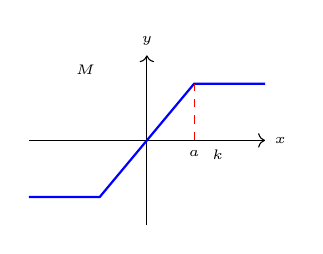
\begin{tikzpicture}[scale=0.6]
\draw[->] (-2.5,0) -- (2.5,0) node[right] {\tiny $x$};
\draw[->] (0,-1.8) -- (0,1.8) node[above] {\tiny $y$};
\draw[blue, thick] (-2.5,-1.2) -- (-1,-1.2) -- (1,1.2) -- (2.5,1.2);
\node at (1.5,-0.3) {\tiny $k$};
\node at (-1.3,1.5) {\tiny $M$};
\draw[dashed, red] (1,0) -- (1,1.2);
\node[below] at (1,0) {\tiny $a$};
\end{tikzpicture}
\end{center}

\begin{align*}
N(A) = \begin{cases}
k & A \leq a \\
\frac{2k}{\pi}\left[\arcsin\frac{a}{A} + \frac{a}{A}\sqrt{1-\left(\frac{a}{A}\right)^2}\right] & A > a
\end{cases}
\end{align*}

其中 $a = M/k$(饱和阈值)

\textbf{2. 死区特性}

\begin{align*}
N(A) = \begin{cases}
0 & A \leq \Delta \\
\frac{k}{\pi}\left[\pi - 2\arcsin\frac{\Delta}{A} - \frac{2\Delta}{A}\sqrt{1-\left(\frac{\Delta}{A}\right)^2}\right] & A > \Delta
\end{cases}
\end{align*}

\textbf{3. 继电特性}

\begin{align*}
N(A) = \frac{4M}{\pi A}
\end{align*}

$M$ 为继电器输出幅值
\end{minipage}

\subsubsection{稳定性分析}

\textbf{闭环系统结构:}

非线性环节 $N(A)$ 串联线性部分 $G(j\omega)$ 构成单位负反馈系统。

\textbf{稳定性判据(类似奈奎斯特判据):}

系统稳定的条件:
\begin{align*}
G(j\omega) \text{曲线不包围点} \left(-\frac{1}{N(A)}\right)
\end{align*}

\textbf{极限环判断:}

极限环存在的条件:
\begin{align*}
G(j\omega_0) = -\frac{1}{N(A_0)}
\end{align*}

此时系统产生频率为 $\omega_0$、幅值为 $A_0$ 的自激振荡。

\vspace{0.3cm}
\textbf{稳定性判断:}

\begin{itemize}
    \item 若 $-1/N(A)$ 曲线在 $G(j\omega)$ 外侧:稳定
    \item 若相交:存在极限环
    \item 极限环稳定性:由交点处曲线的相对位置决定
\end{itemize}

\vspace{0.3cm}
\textbf{例题:}系统含继电特性 $M=1$,线性部分 $G(s) = \frac{K}{s(s+1)}$,$K=2$,判断是否存在极限环。

\textit{解:}

\textbf{1. 继电特性的描述函数}
\begin{align*}
N(A) = \frac{4M}{\pi A} = \frac{4}{\pi A}
\end{align*}

\textbf{2. $-1/N(A)$ 曲线}
\begin{align*}
-\frac{1}{N(A)} = -\frac{\pi A}{4}
\end{align*}

这是实轴上的负半轴,$A$ 从 $0$ 到 $\infty$ 变化时,点从 $0$ 到 $-\infty$ 移动。

\textbf{3. $G(j\omega)$ 曲线}
\begin{align*}
G(j\omega) = \frac{2}{j\omega(1+j\omega)} = \frac{2(1-j\omega)}{\omega^2(1+\omega^2)}
\end{align*}

\textbf{4. 交点判断}

令 $\text{Im}[G(j\omega)] = 0$:$-2/[\omega^2(1+\omega^2)] = 0$ 无解

$G(j\omega)$ 曲线不与实轴负半轴相交 $\implies$ 不存在极限环。

\textbf{结论:}系统不会产生自激振荡。

\subsection{Lyapunov稳定性理论(非线性系统)}

Lyapunov第二方法(直接法)适用于非线性系统的稳定性分析,无需求解微分方程。

\subsubsection{Lyapunov稳定性定义}

考虑非线性系统:
\begin{align*}
\dot{\mathbf{x}} = \mathbf{f}(\mathbf{x}, t)
\end{align*}

假设 $\mathbf{x}_e$ 是平衡点($\mathbf{f}(\mathbf{x}_e, t) = 0$)。

\textbf{稳定性定义:}

\begin{itemize}
    \item \textbf{稳定}:对任意 $\epsilon > 0$,存在 $\delta > 0$,使得当 $\|\mathbf{x}(0) - \mathbf{x}_e\| < \delta$ 时,有 $\|\mathbf{x}(t) - \mathbf{x}_e\| < \epsilon$($t \geq 0$)
    \item \textbf{渐近稳定}:稳定且 $\lim_{t\to\infty} \mathbf{x}(t) = \mathbf{x}_e$
    \item \textbf{全局渐近稳定}:对任意初始条件都渐近稳定
\end{itemize}

\subsubsection{Lyapunov定理}

\textbf{定理(Lyapunov稳定性定理):}

如果存在标量函数 $V(\mathbf{x})$(Lyapunov函数)满足:

\begin{enumerate}
    \item $V(\mathbf{x})$ 连续可微
    \item $V(\mathbf{x}_e) = 0$ 且在 $\mathbf{x} \neq \mathbf{x}_e$ 时 $V(\mathbf{x}) > 0$(正定)
    \item $\dot{V}(\mathbf{x}) = \frac{\partial V}{\partial \mathbf{x}} \cdot \mathbf{f}(\mathbf{x}, t) \leq 0$(半负定)
\end{enumerate}

则平衡点 $\mathbf{x}_e$ 是\textbf{稳定}的。

如果进一步满足:
\begin{enumerate}
    \setcounter{enumi}{3}
    \item $\dot{V}(\mathbf{x}) < 0$($\mathbf{x} \neq \mathbf{x}_e$,负定)
\end{enumerate}

则平衡点 $\mathbf{x}_e$ 是\textbf{渐近稳定}的。

\vspace{0.3cm}
\textbf{Lyapunov函数的构造:}

常用形式(二次型):
\begin{align*}
V(\mathbf{x}) = \mathbf{x}^T \mathbf{P} \mathbf{x}
\end{align*}

其中 $\mathbf{P}$ 是正定对称矩阵。

\vspace{0.3cm}
\textbf{例题:}分析系统 $\dot{x}_1 = x_2$,$\dot{x}_2 = -x_1 - x_2$ 的稳定性。

\textit{解:}

\textbf{1. 确定平衡点}

令 $\dot{x}_1 = \dot{x}_2 = 0$:$x_1 = x_2 = 0$

\textbf{2. 构造Lyapunov函数}

选择:$V(x_1, x_2) = x_1^2 + x_2^2$

\textbf{3. 验证正定性}

$V(0, 0) = 0$ 且 $V(x_1, x_2) > 0$($x_1, x_2$ 不全为零)$\implies$ 正定

\textbf{4. 计算 $\dot{V}$}
\begin{align*}
\dot{V} &= \frac{\partial V}{\partial x_1}\dot{x}_1 + \frac{\partial V}{\partial x_2}\dot{x}_2 \\
&= 2x_1 \cdot x_2 + 2x_2 \cdot (-x_1 - x_2) \\
&= 2x_1 x_2 - 2x_1 x_2 - 2x_2^2 \\
&= -2x_2^2 \leq 0
\end{align*}

$\dot{V} < 0$(除原点外)$\implies$ 负定

\textbf{结论:}原点是\textbf{渐近稳定}的平衡点。

\subsection{总结}

\begin{center}
\begin{tabular}{|l|p{4cm}|p{4cm}|p{3cm}|}
\hline
\textbf{方法} & \textbf{适用范围} & \textbf{优点} & \textbf{缺点} \\
\hline
相平面法 & 二阶系统 & 直观、图形化 & 仅限二阶 \\
\hline
描述函数法 & 含单一非线性环节 & 频域分析、预测极限环 & 近似方法 \\
\hline
Lyapunov法 & 任意阶非线性系统 & 严格、不需求解方程 & 构造函数困难 \\
\hline
\end{tabular}
\end{center}

\section{离散系统}
\label{sec:discrete-systems}

\subsection{离散系统概述}

\subsubsection{离散系统的定义}

\textbf{离散系统}(数字控制系统)是指信号在时间上离散,通常涉及采样、数字处理和保持等环节。

\begin{minipage}[t]{0.52\textwidth}
\textbf{连续系统 vs 离散系统:}

\textbf{连续系统:}
\begin{itemize}
    \item 信号连续变化
    \item 微分方程描述
    \item 拉普拉斯变换分析
\end{itemize}

\textbf{离散系统:}
\begin{itemize}
    \item 信号在采样时刻定义
    \item 差分方程描述
    \item Z变换分析
\end{itemize}

\vspace{0.3cm}
\textbf{离散系统的组成:}

\begin{enumerate}
    \item \textbf{采样器}:将连续信号转换为离散序列
    \item \textbf{数字控制器}:对离散信号进行数字处理
    \item \textbf{保持器}:将离散信号还原为连续信号
    \item \textbf{被控对象}:连续系统
\end{enumerate}

\vspace{0.3cm}
\textbf{采样定理(Nyquist-Shannon定理):}

为无失真恢复连续信号,采样频率必须:
\begin{align*}
f_s \geq 2f_{\max}
\end{align*}

或采样周期:
\begin{align*}
T \leq \frac{\pi}{\omega_{\max}}
\end{align*}

其中 $f_{\max}$ 是信号的最高频率分量。

\textbf{工程实践:}
\begin{itemize}
    \item 一般取 $f_s = (6 \sim 10) f_{\max}$
    \item 或采样周期 $T = (0.1 \sim 0.5) T_s$($T_s$ 为系统时间常数)
\end{itemize}
\end{minipage}\hfill
\begin{minipage}[t]{0.45\textwidth}
\vspace{0pt}
\textbf{离散控制系统结构:}

离散控制系统包含以下环节:
\begin{itemize}
    \item 采样器(周期 $T$)
    \item 数字控制器
    \item 保持器(通常为零阶保持器)
    \item 被控对象(连续系统)
\end{itemize}

采样器将连续信号在离散时刻采样,数字控制器对离散信号进行处理,保持器将离散信号还原为阶梯波形式的连续信号,最后作用于被控对象。

\vspace{0.3cm}
\textbf{采样过程:}

采样过程将连续信号 $r(t)$ 在时刻 $t = kT$($k=0,1,2,\ldots$)进行采样,得到离散序列 $r(kT)$。
\end{minipage}

\subsection{Z变换}

Z变换是分析离散系统的数学工具,类似于连续系统中的拉普拉斯变换。

\subsubsection{Z变换的定义}

对于离散序列 $\{f(kT)\}$($k = 0, 1, 2, \ldots$),其Z变换定义为:
\begin{align*}
F(z) = \mathcal{Z}\{f(kT)\} = \sum_{k=0}^{\infty} f(kT) z^{-k}
\end{align*}

其中 $z$ 是复变量。

\subsubsection{Z变换与拉氏变换的关系}

对于采样信号 $f^*(t) = \sum_{k=0}^{\infty} f(kT)\delta(t-kT)$,其拉氏变换为:
\begin{align*}
F^*(s) = \sum_{k=0}^{\infty} f(kT) e^{-skT}
\end{align*}

令 $z = e^{sT}$,则:
\begin{align*}
F(z) = F^*(s)\Big|_{z=e^{sT}}
\end{align*}

\textbf{$s$ 平面与 $z$ 平面的映射:}

\begin{center}
\begin{tikzpicture}[scale=0.7]
% s平面
\begin{scope}[shift={(0,0)}]
\draw[->] (-2,0) -- (2,0) node[right] {$\text{Re}(s)$};
\draw[->] (0,-2) -- (0,2) node[above] {$\text{Im}(s)$};
\draw[blue, thick] (-2,-2) -- (-2,2);
\draw[red, thick] (0,-2) -- (0,2);
\node[blue, left] at (-2,1.5) {不稳定};
\node[red, right] at (0,1.5) {稳定};
\node[below] at (0,-2.5) {$s$ 平面};
\end{scope}

% 箭头
\draw[->, thick] (2.5,0) -- (3.5,0) node[midway, above] {\small $z=e^{sT}$};

% z平面
\begin{scope}[shift={(6,0)}]
\draw[->] (-2,0) -- (2,0) node[right] {$\text{Re}(z)$};
\draw[->] (0,-2) -- (0,2) node[above] {$\text{Im}(z)$};
\draw[thick] (0,0) circle (1);
\fill[blue, opacity=0.2] (0,0) circle (1);
\node[red] at (1.5,0) {不稳定};
\node[blue] at (0.5,0.5) {稳定};
\node[below] at (0,-2.5) {$z$ 平面};
\end{scope}
\end{tikzpicture}
\end{center}

\textbf{关键对应关系:}
\begin{itemize}
    \item $s$ 平面左半平面 $\leftrightarrow$ $z$ 平面单位圆内
    \item $s$ 平面虚轴 $\leftrightarrow$ $z$ 平面单位圆上
    \item $s$ 平面右半平面 $\leftrightarrow$ $z$ 平面单位圆外
\end{itemize}

\subsubsection{常用序列的Z变换}

\begin{center}
\begin{tabular}{|c|c|c|}
\hline
\textbf{序列} $f(kT)$ & \textbf{Z变换} $F(z)$ & \textbf{收敛域} \\
\hline
$\delta(kT)$(单位脉冲) & $1$ & 全平面 \\
\hline
$1(kT)$(单位阶跃) & $\frac{z}{z-1}$ & $|z| > 1$ \\
\hline
$kT$ & $\frac{Tz}{(z-1)^2}$ & $|z| > 1$ \\
\hline
$e^{-akT}$ & $\frac{z}{z-e^{-aT}}$ & $|z| > e^{-aT}$ \\
\hline
$\sin(\omega kT)$ & $\frac{z\sin(\omega T)}{z^2 - 2z\cos(\omega T) + 1}$ & $|z| > 1$ \\
\hline
$\cos(\omega kT)$ & $\frac{z[z-\cos(\omega T)]}{z^2 - 2z\cos(\omega T) + 1}$ & $|z| > 1$ \\
\hline
$a^k$ & $\frac{z}{z-a}$ & $|z| > |a|$ \\
\hline
$ka^k$ & $\frac{az}{(z-a)^2}$ & $|z| > |a|$ \\
\hline
\end{tabular}
\end{center}

\subsubsection{Z变换的性质}

\begin{center}
\begin{tabular}{|l|c|c|}
\hline
\textbf{性质} & \textbf{时域} & \textbf{Z域} \\
\hline
线性 & $a f_1(kT) + b f_2(kT)$ & $a F_1(z) + b F_2(z)$ \\
\hline
右移 & $f(kT - nT)$ & $z^{-n} F(z)$ \\
\hline
左移 & $f(kT + nT)$ & $z^n [F(z) - \sum_{k=0}^{n-1} f(kT) z^{-k}]$ \\
\hline
初值定理 & $f(0)$ & $\lim_{z\to\infty} F(z)$ \\
\hline
终值定理 & $\lim_{k\to\infty} f(kT)$ & $\lim_{z\to 1} (z-1)F(z)$ \\
\hline
卷积 & $\sum_{i=0}^k f_1(iT) f_2(kT-iT)$ & $F_1(z) \cdot F_2(z)$ \\
\hline
\end{tabular}
\end{center}

\subsection{脉冲传递函数}

\subsubsection{定义}

脉冲传递函数是离散系统的输出Z变换与输入Z变换之比(零初始条件):
\begin{align*}
G(z) = \frac{Y(z)}{X(z)}
\end{align*}

\subsubsection{零阶保持器(ZOH)}

零阶保持器在采样周期内保持采样值不变。

\begin{minipage}[t]{0.52\textwidth}
\textbf{零阶保持器的传递函数:}
\begin{align*}
G_h(s) = \frac{1 - e^{-Ts}}{s}
\end{align*}

\textbf{含零阶保持器的系统:}

采样器 + ZOH + 连续对象 $G(s)$

等效脉冲传递函数:
\begin{align*}
G(z) = \mathcal{Z}\left\{\frac{1-e^{-Ts}}{s} G(s)\right\} = (1-z^{-1})\mathcal{Z}\left\{\frac{G(s)}{s}\right\}
\end{align*}

\vspace{0.3cm}
\textbf{常用公式:}

对于 $G(s) = \frac{1}{s+a}$:
\begin{align*}
G(z) = (1-z^{-1})\mathcal{Z}\left\{\frac{1}{s(s+a)}\right\} = \frac{1-e^{-aT}}{z-e^{-aT}}
\end{align*}

对于 $G(s) = \frac{1}{s(s+a)}$:
\begin{align*}
G(z) = (1-z^{-1})\mathcal{Z}\left\{\frac{1}{s^2(s+a)}\right\} = \frac{T - \frac{1-e^{-aT}}{a}}{(z-1)(z-e^{-aT})}
\end{align*}
\end{minipage}\hfill
\begin{minipage}[t]{0.45\textwidth}
\vspace{0pt}
\textbf{零阶保持器输出示意:}

零阶保持器(Zero-Order Hold, ZOH)在每个采样周期内保持采样值不变,将离散信号转换为阶梯波形式的连续信号。

输出特点:
\begin{itemize}
    \item 在每个采样周期 $[kT, (k+1)T)$ 内,输出保持为 $y(kT)$
    \item 在采样时刻发生跳变
    \item 形成阶梯波形
\end{itemize}

\vspace{0.5cm}
\textbf{例题:}求含ZOH和对象 $G(s) = \frac{1}{s+2}$ 的脉冲传递函数,$T = 0.1$ s。

\textit{解:}

\textbf{方法1:查表法}
\begin{align*}
G(z) &= (1-z^{-1})\mathcal{Z}\left\{\frac{1}{s(s+2)}\right\} \\
&= \frac{1-e^{-2T}}{z-e^{-2T}} \\
&= \frac{1-e^{-0.2}}{z-e^{-0.2}} \\
&= \frac{0.1813}{z-0.8187}
\end{align*}

\textbf{方法2:部分分式法}
\begin{align*}
\frac{G(s)}{s} &= \frac{1}{s(s+2)} = \frac{0.5}{s} - \frac{0.5}{s+2} \\
\mathcal{Z}\left\{\frac{1}{s(s+2)}\right\} &= 0.5\frac{z}{z-1} - 0.5\frac{z}{z-e^{-2T}} \\
G(z) &= (1-z^{-1}) \times \text{上式} \\
&= \frac{0.1813}{z-0.8187}
\end{align*}
\end{minipage}

\subsection{离散系统的稳定性}

\subsubsection{稳定性判据}

离散系统稳定的充要条件:闭环脉冲传递函数 $\Phi(z)$ 的所有极点都在 $z$ 平面单位圆内,即:
\begin{align*}
|z_i| < 1, \quad i = 1, 2, \ldots, n
\end{align*}

\subsubsection{劳斯判据的应用(双线性变换)}

通过双线性变换 $z = \frac{1+w}{1-w}$,将 $z$ 平面单位圆内映射到 $w$ 平面左半平面,然后应用劳斯判据。

\textbf{步骤:}

1. 求闭环特征方程 $D(z) = 0$

2. 进行双线性变换:$z = \frac{1+w}{1-w}$,得 $D(w) = 0$

3. 对 $D(w) = 0$ 应用劳斯判据

\vspace{0.3cm}
\textbf{例题:}判断系统 $\Phi(z) = \frac{K}{z^2 - 1.5z + 0.5}$ 的稳定性,$K = 1$。

\textit{解:}

\textbf{1. 特征方程}
\begin{align*}
D(z) = z^2 - 1.5z + 0.5 + K = z^2 - 1.5z + 1.5 = 0
\end{align*}

\textbf{2. 双线性变换}

令 $z = \frac{1+w}{1-w}$:
\begin{align*}
\left(\frac{1+w}{1-w}\right)^2 - 1.5\frac{1+w}{1-w} + 1.5 &= 0 \\
(1+w)^2 - 1.5(1+w)(1-w) + 1.5(1-w)^2 &= 0 \\
1 + 2w + w^2 - 1.5(1-w^2) + 1.5(1-2w+w^2) &= 0 \\
1 + 2w + w^2 - 1.5 + 1.5w^2 + 1.5 - 3w + 1.5w^2 &= 0 \\
4w^2 - w + 1 &= 0
\end{align*}

\textbf{3. 劳斯表}
\begin{center}
\begin{tabular}{c|cc}
$w^2$ & 4 & 1 \\
$w^1$ & -1 & 0 \\
$w^0$ & 1 &  \\
\end{tabular}
\end{center}

第一列有符号变化(+,-,+)$\implies$ \textbf{不稳定}

\textbf{验证:}直接求根:$z = \frac{1.5 \pm \sqrt{2.25-6}}{2} = 0.75 \pm 0.968j$,$|z| = 1.22 > 1$

\subsubsection{Jury稳定性判据}

Jury判据直接在 $z$ 域判断稳定性,无需变换。

设特征方程:
\begin{align*}
D(z) = a_0 z^n + a_1 z^{n-1} + \cdots + a_{n-1} z + a_n = 0
\end{align*}

\textbf{稳定的必要条件:}
\begin{align*}
D(1) > 0, \quad (-1)^n D(-1) > 0
\end{align*}

\textbf{充要条件:}构造Jury表,所有行的首元素满足特定符号条件。

(详细方法略,工程中常用数值计算求根判断)

\subsection{离散系统的动态性能}

\subsubsection{稳态误差}

\textbf{终值定理:}
\begin{align*}
e_{ss} = \lim_{k\to\infty} e(kT) = \lim_{z\to 1} (z-1)E(z)
\end{align*}

\textbf{单位阶跃输入:}$R(z) = \frac{z}{z-1}$
\begin{align*}
e_{ss} = \lim_{z\to 1} (z-1) \frac{R(z)}{1+G(z)} = \frac{1}{1 + \lim_{z\to 1} G(z)}
\end{align*}

\textbf{单位斜坡输入:}$R(z) = \frac{Tz}{(z-1)^2}$
\begin{align*}
e_{ss} = \lim_{z\to 1} (z-1) \frac{Tz}{(z-1)^2[1+G(z)]} = \frac{T}{\lim_{z\to 1} (z-1)G(z)/T}
\end{align*}

\subsubsection{瞬态性能指标}

离散系统的时域响应可以通过Z反变换求得:
\begin{align*}
y(kT) = \mathcal{Z}^{-1}\{Y(z)\}
\end{align*}

\textbf{常用方法:}
\begin{itemize}
    \item \textbf{长除法}:直接展开为序列
    \item \textbf{部分分式法}:分解后查表反变换
    \item \textbf{留数法}:复变函数理论
\end{itemize}

\textbf{性能指标:}
\begin{itemize}
    \item 上升时间 $t_r$
    \item 超调量 $\sigma\%$
    \item 调节时间 $t_s$
    \item 振荡次数
\end{itemize}

\subsection{数字PID控制}

\subsubsection{连续PID的离散化}

连续PID控制器:
\begin{align*}
u(t) = K_p e(t) + K_i \int_0^t e(\tau) d\tau + K_d \frac{de(t)}{dt}
\end{align*}

\textbf{位置式数字PID:}
\begin{align*}
u(k) = K_p e(k) + K_i T \sum_{j=0}^k e(j) + K_d \frac{e(k) - e(k-1)}{T}
\end{align*}

\textbf{速度式数字PID:}
\begin{align*}
\Delta u(k) = u(k) - u(k-1) &= K_p [e(k) - e(k-1)] \\
&\quad + K_i T e(k) \\
&\quad + K_d \frac{e(k) - 2e(k-1) + e(k-2)}{T}
\end{align*}

\subsubsection{数字PID的改进}

\textbf{1. 积分分离}:误差大时不积分,避免积分饱和
\begin{align*}
u(k) = K_p e(k) + K_i T \sum_{j=k_0}^k e(j) + K_d \frac{e(k) - e(k-1)}{T}
\end{align*}

\textbf{2. 微分先行}:仅对输出微分,避免对设定值突变响应过大
\begin{align*}
u(k) = K_p e(k) + K_i T \sum_{j=0}^k e(j) - K_d \frac{y(k) - y(k-1)}{T}
\end{align*}

\textbf{3. 不完全微分}:加入滤波环节,减小噪声影响
\begin{align*}
u_d(k) = \alpha u_d(k-1) + K_d (1-\alpha) \frac{e(k) - e(k-1)}{T}
\end{align*}

其中 $\alpha = \frac{T}{T + \tau_d}$,$\tau_d$ 为滤波时间常数。

\subsection{离散系统设计}

\subsubsection{最少拍控制}

\textbf{设计目标:}在最少的采样周期内使系统输出达到并保持在期望值。

\textbf{设计步骤:}

1. 确定期望闭环传递函数 $\Phi^*(z)$

2. 计算控制器传递函数:
\begin{align*}
D(z) = \frac{\Phi^*(z)}{G(z)[1-\Phi^*(z)]}
\end{align*}

3. 验证物理可实现性和稳定性

\textbf{常用期望响应:}
\begin{itemize}
    \item 单拍系统:$\Phi^*(z) = z^{-1}$
    \item 有纹波最少拍:$\Phi^*(z) = \frac{(1-a)z^{-1}}{1-az^{-1}}$
    \item 无纹波最少拍(I型系统):$\Phi^*(z) = z^{-1}(2-z^{-1})$
\end{itemize}

\subsubsection{数字控制器的实现}

\textbf{直接编程法:}

控制器传递函数 $D(z) = \frac{U(z)}{E(z)}$ 转换为差分方程,直接编程实现。

\textbf{串行校正:}

类似连续系统的超前/滞后校正,设计数字校正器:
\begin{align*}
D(z) = K \frac{z - a}{z - b}
\end{align*}

\textbf{并行校正:}

采用状态反馈等现代控制方法。

\subsection{总结}

\begin{center}
\begin{tabular}{|l|c|c|}
\hline
\textbf{特性} & \textbf{连续系统} & \textbf{离散系统} \\
\hline
数学描述 & 微分方程 & 差分方程 \\
\hline
变换工具 & 拉普拉斯变换 & Z变换 \\
\hline
频域函数 & 传递函数 $G(s)$ & 脉冲传递函数 $G(z)$ \\
\hline
稳定域 & $s$ 平面左半平面 & $z$ 平面单位圆内 \\
\hline
稳定判据 & 劳斯、奈奎斯特 & 双线性变换+劳斯、Jury \\
\hline
控制器 & 模拟PID & 数字PID、最少拍 \\
\hline
\end{tabular}
\end{center}

\textbf{离散系统设计要点:}
\begin{enumerate}
    \item 选择合适的采样周期(满足采样定理,通常 $T = 0.1 \sim 0.5$ 时间常数)
    \item 考虑零阶保持器的影响
    \item 数字控制器设计(数字PID、最少拍等)
    \item 验证闭环稳定性(极点在单位圆内)
    \item 评估动态性能(超调、调节时间等)
\end{enumerate}


\end{document}
